\subsection*{Measured raw data}
\setcounter{topnumber}{10}
\setcounter{bottomnumber}{10}
\setcounter{totalnumber}{10}
\renewcommand{\topfraction}{1}
\renewcommand{\bottomfraction}{1}
%\renewcommand{\textfraction}{0.05}
\renewcommand{\floatpagefraction}{1}
%%%%%%%%%%%%%%%%%%%%%%%%%%%%%%%%%%%%
%%% BSA at Vc = 2.5 ml/min
%%%%%%%%%%%%%%%%%%%%%%%%%%%%%%%%%%%%%
\newcommand{\subFigSize}{0.45\linewidth}
%\newcommand{\vertDist}{\vspace*{-1.5ex}}
\begin{figure}[H]
  \begin{center}
    \begin{subfigure}{\subFigSize}
    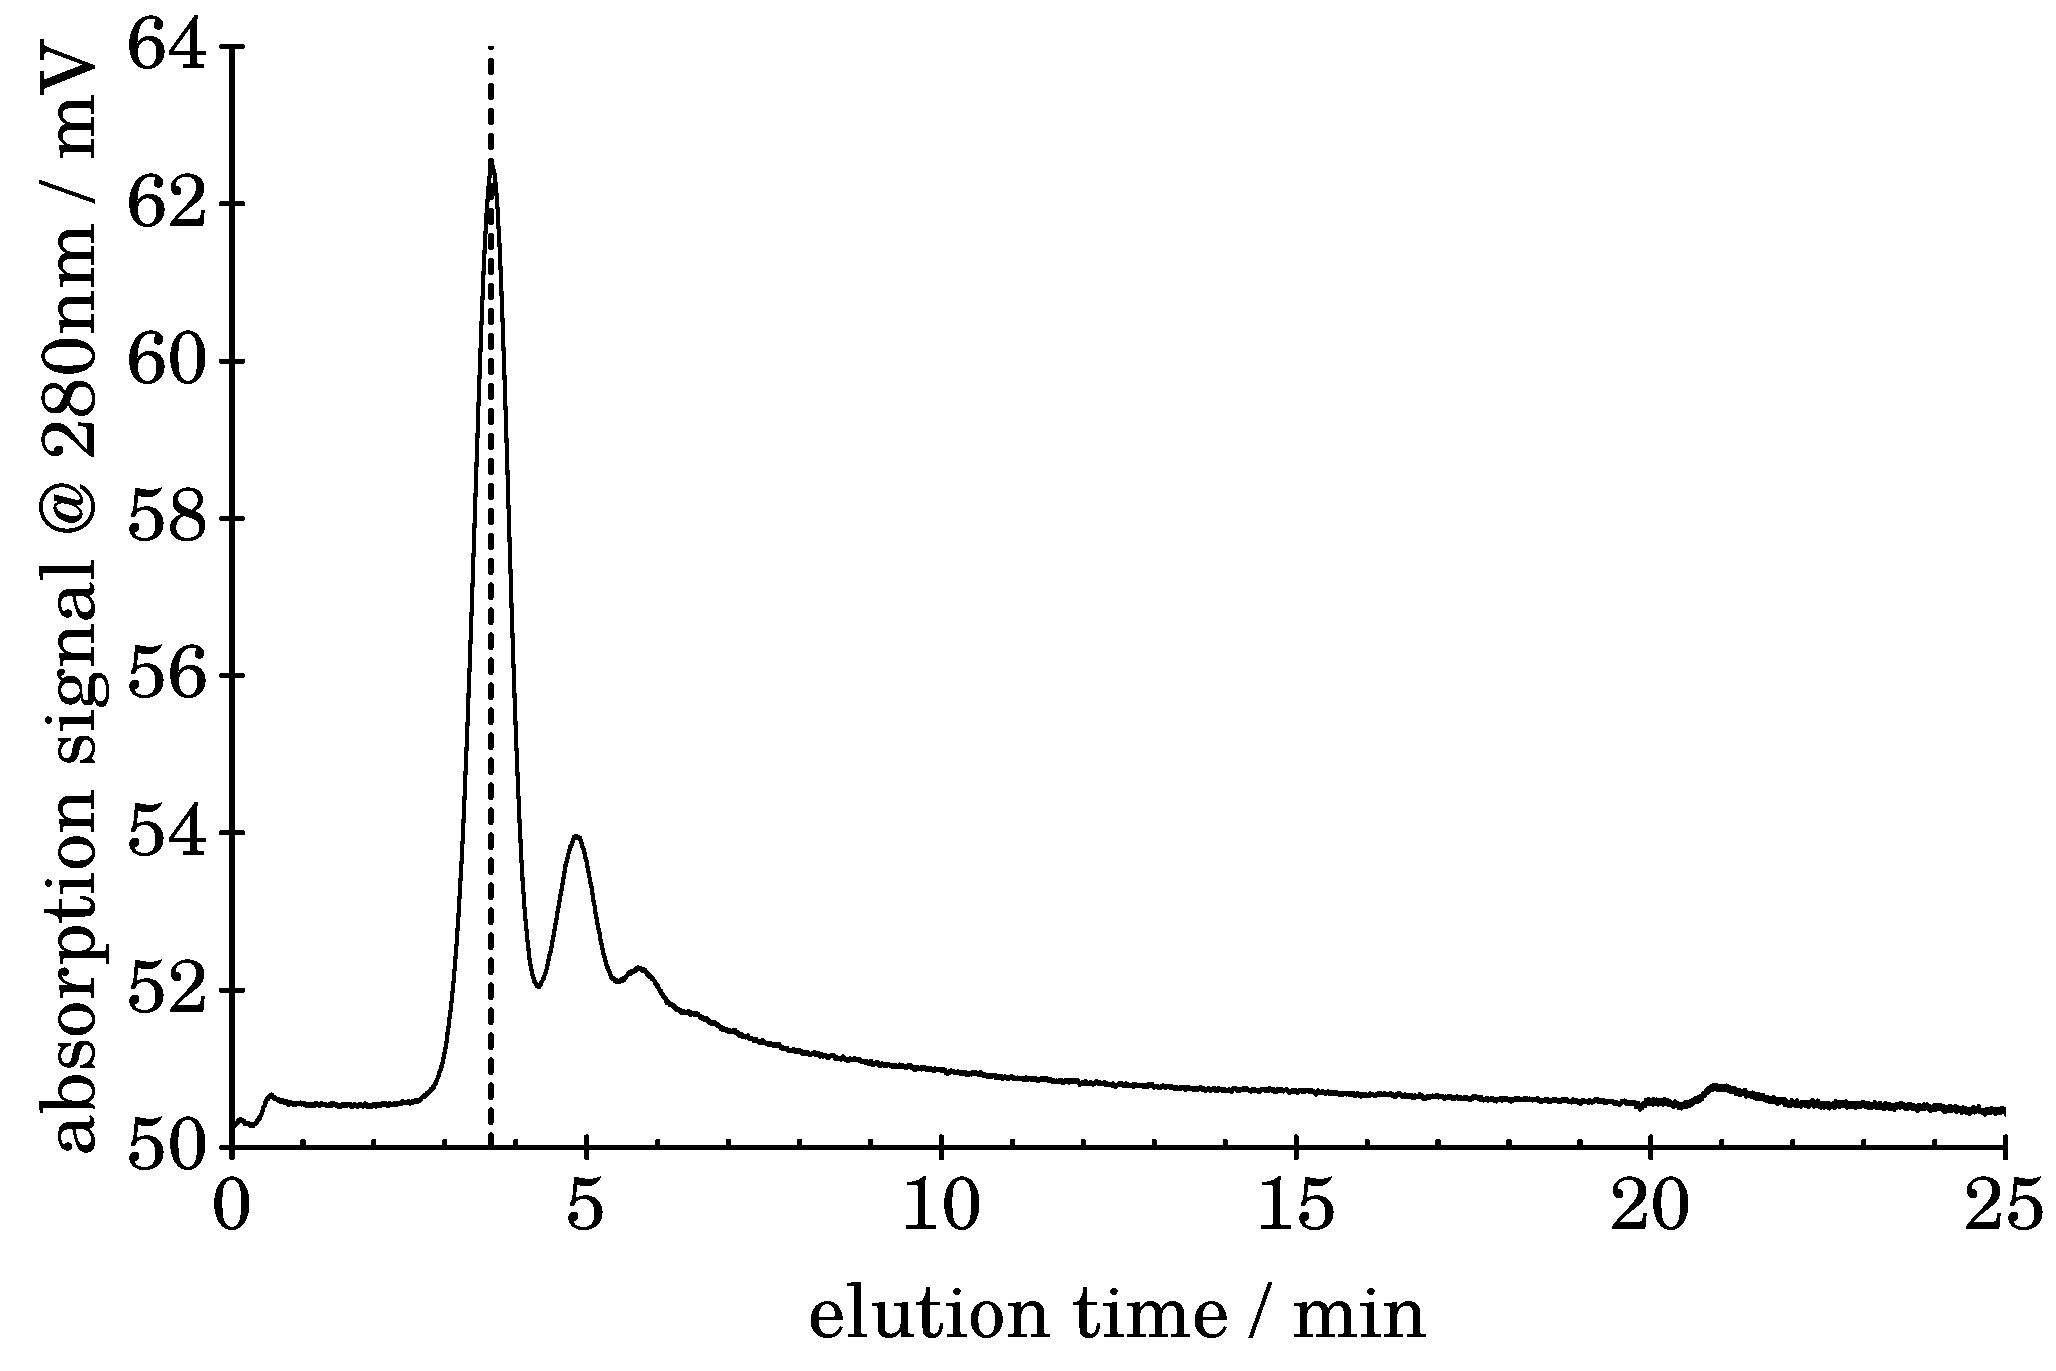
\includegraphics[width=\linewidth]{./images/data/rawPlots/img_BSA_VC_2_5_r1_te.pdf}
      \subcaption{Position of $\te$, replicate 1.}
      \label{subfig:raw_BSA2_5_r1_te}
    \end{subfigure}
      \begin{subfigure}{\subFigSize}
    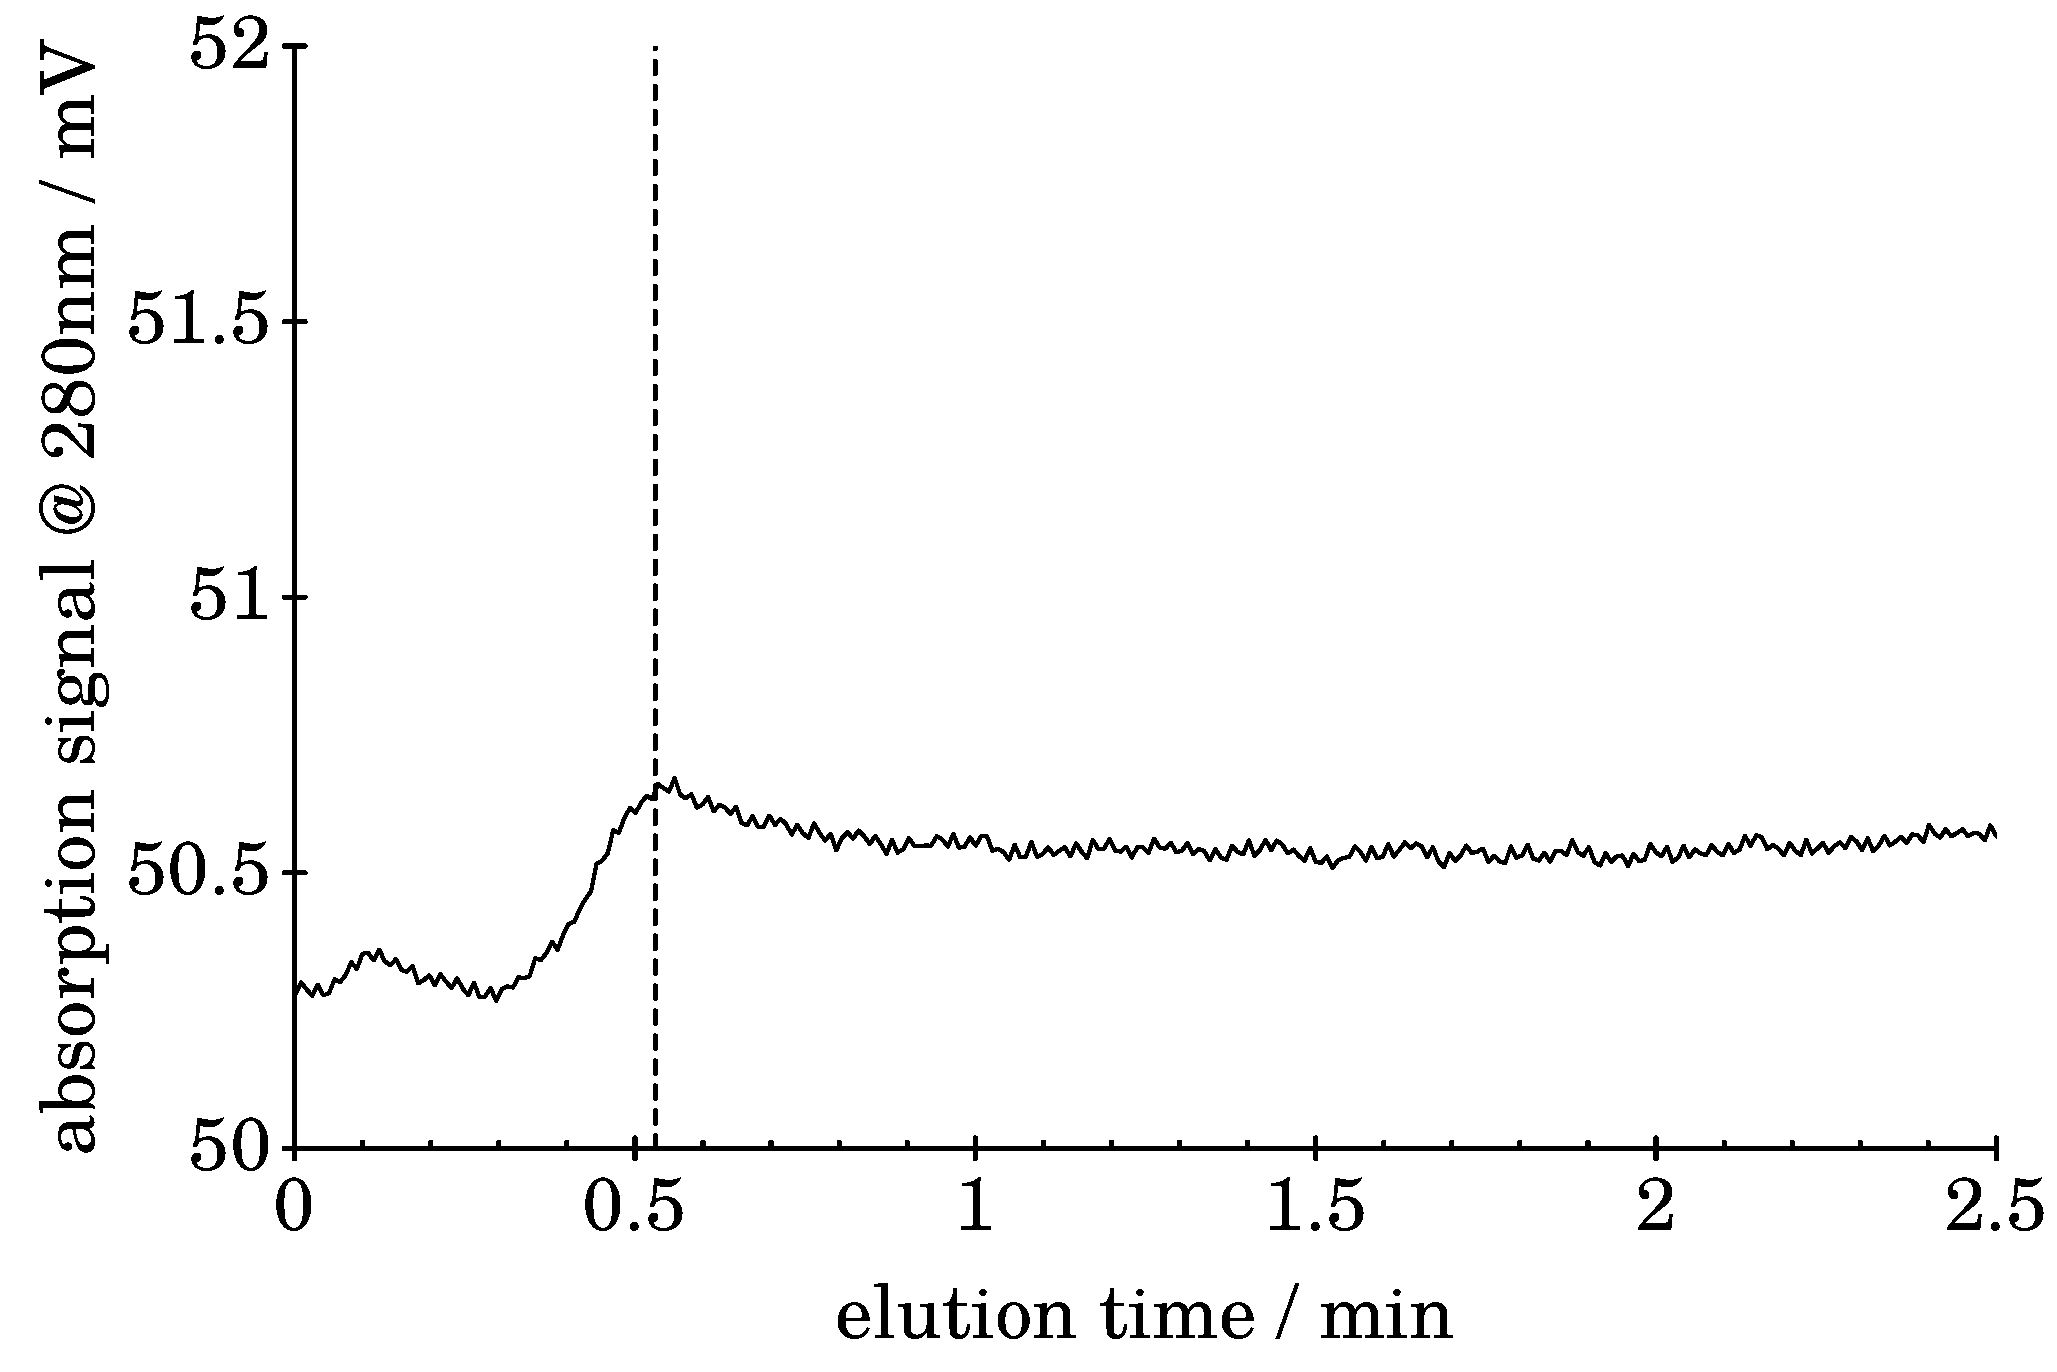
\includegraphics[width=\linewidth]{./images/data/rawPlots/img_BSA_VC_2_5_r1_t0.pdf}
    \subcaption{Detailed starting section of fractogram \ref{subfig:raw_BSA2_5_r1_te};
      Position of $\tvoid$, replicate 1.}
  \end{subfigure}
  \\\vspace*{.5em}
  %%%%%%%%%%%%%%%%%%%%%
      \begin{subfigure}{\subFigSize}
    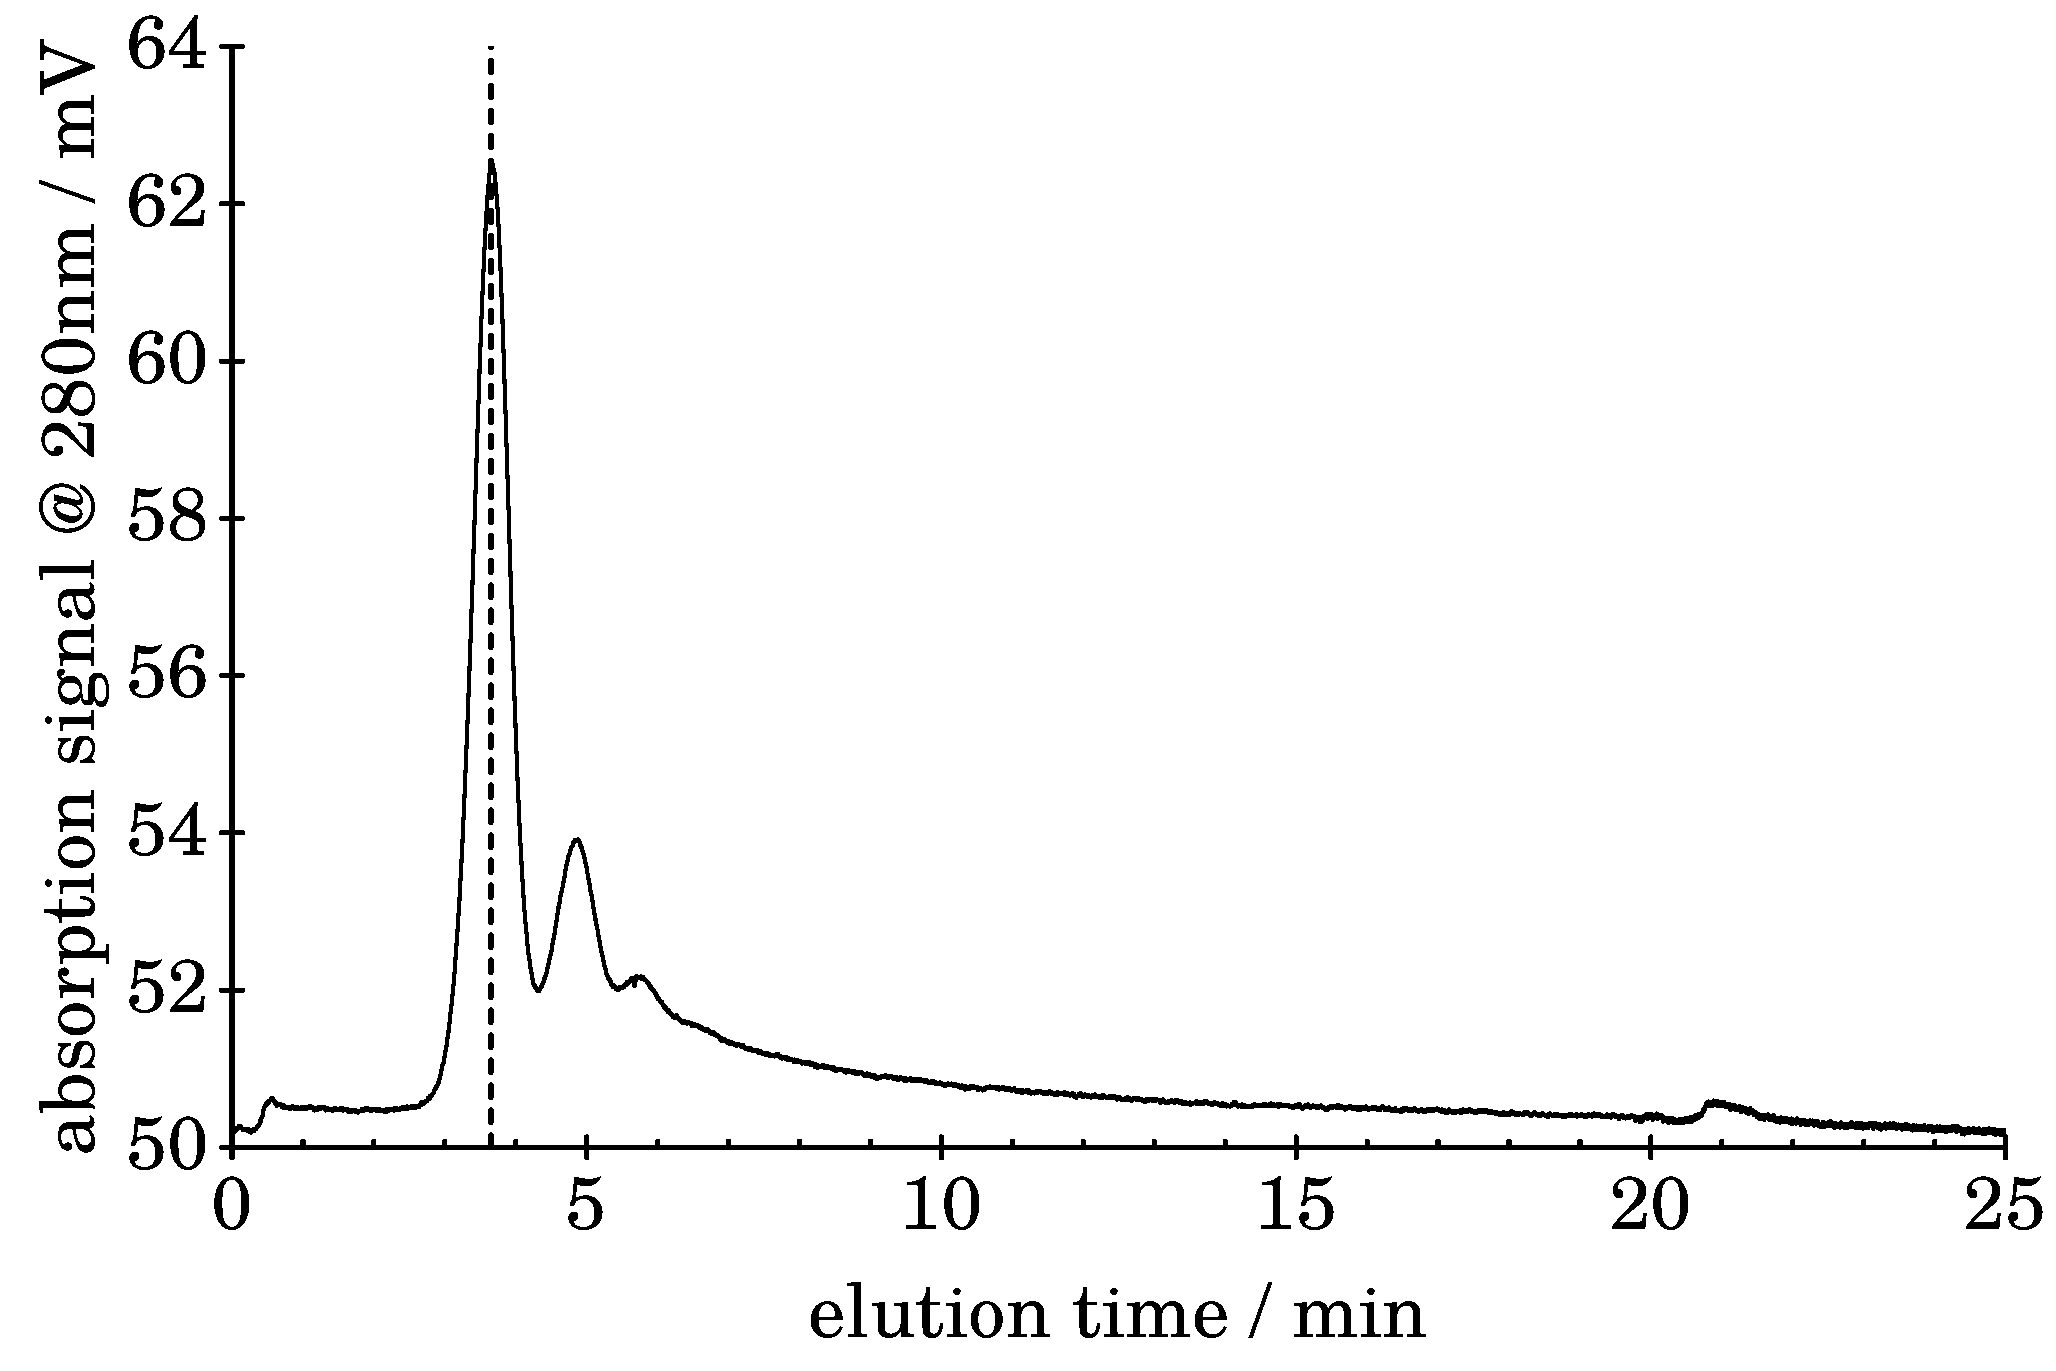
\includegraphics[width=\linewidth]{./images/data/rawPlots/img_BSA_VC_2_5_r2_te.pdf}
    \subcaption{Position of $\te$, replicate 2.}
    \label{subfig:raw_BSA2_5_r2_te}
  \end{subfigure}
  \begin{subfigure}{\subFigSize}
    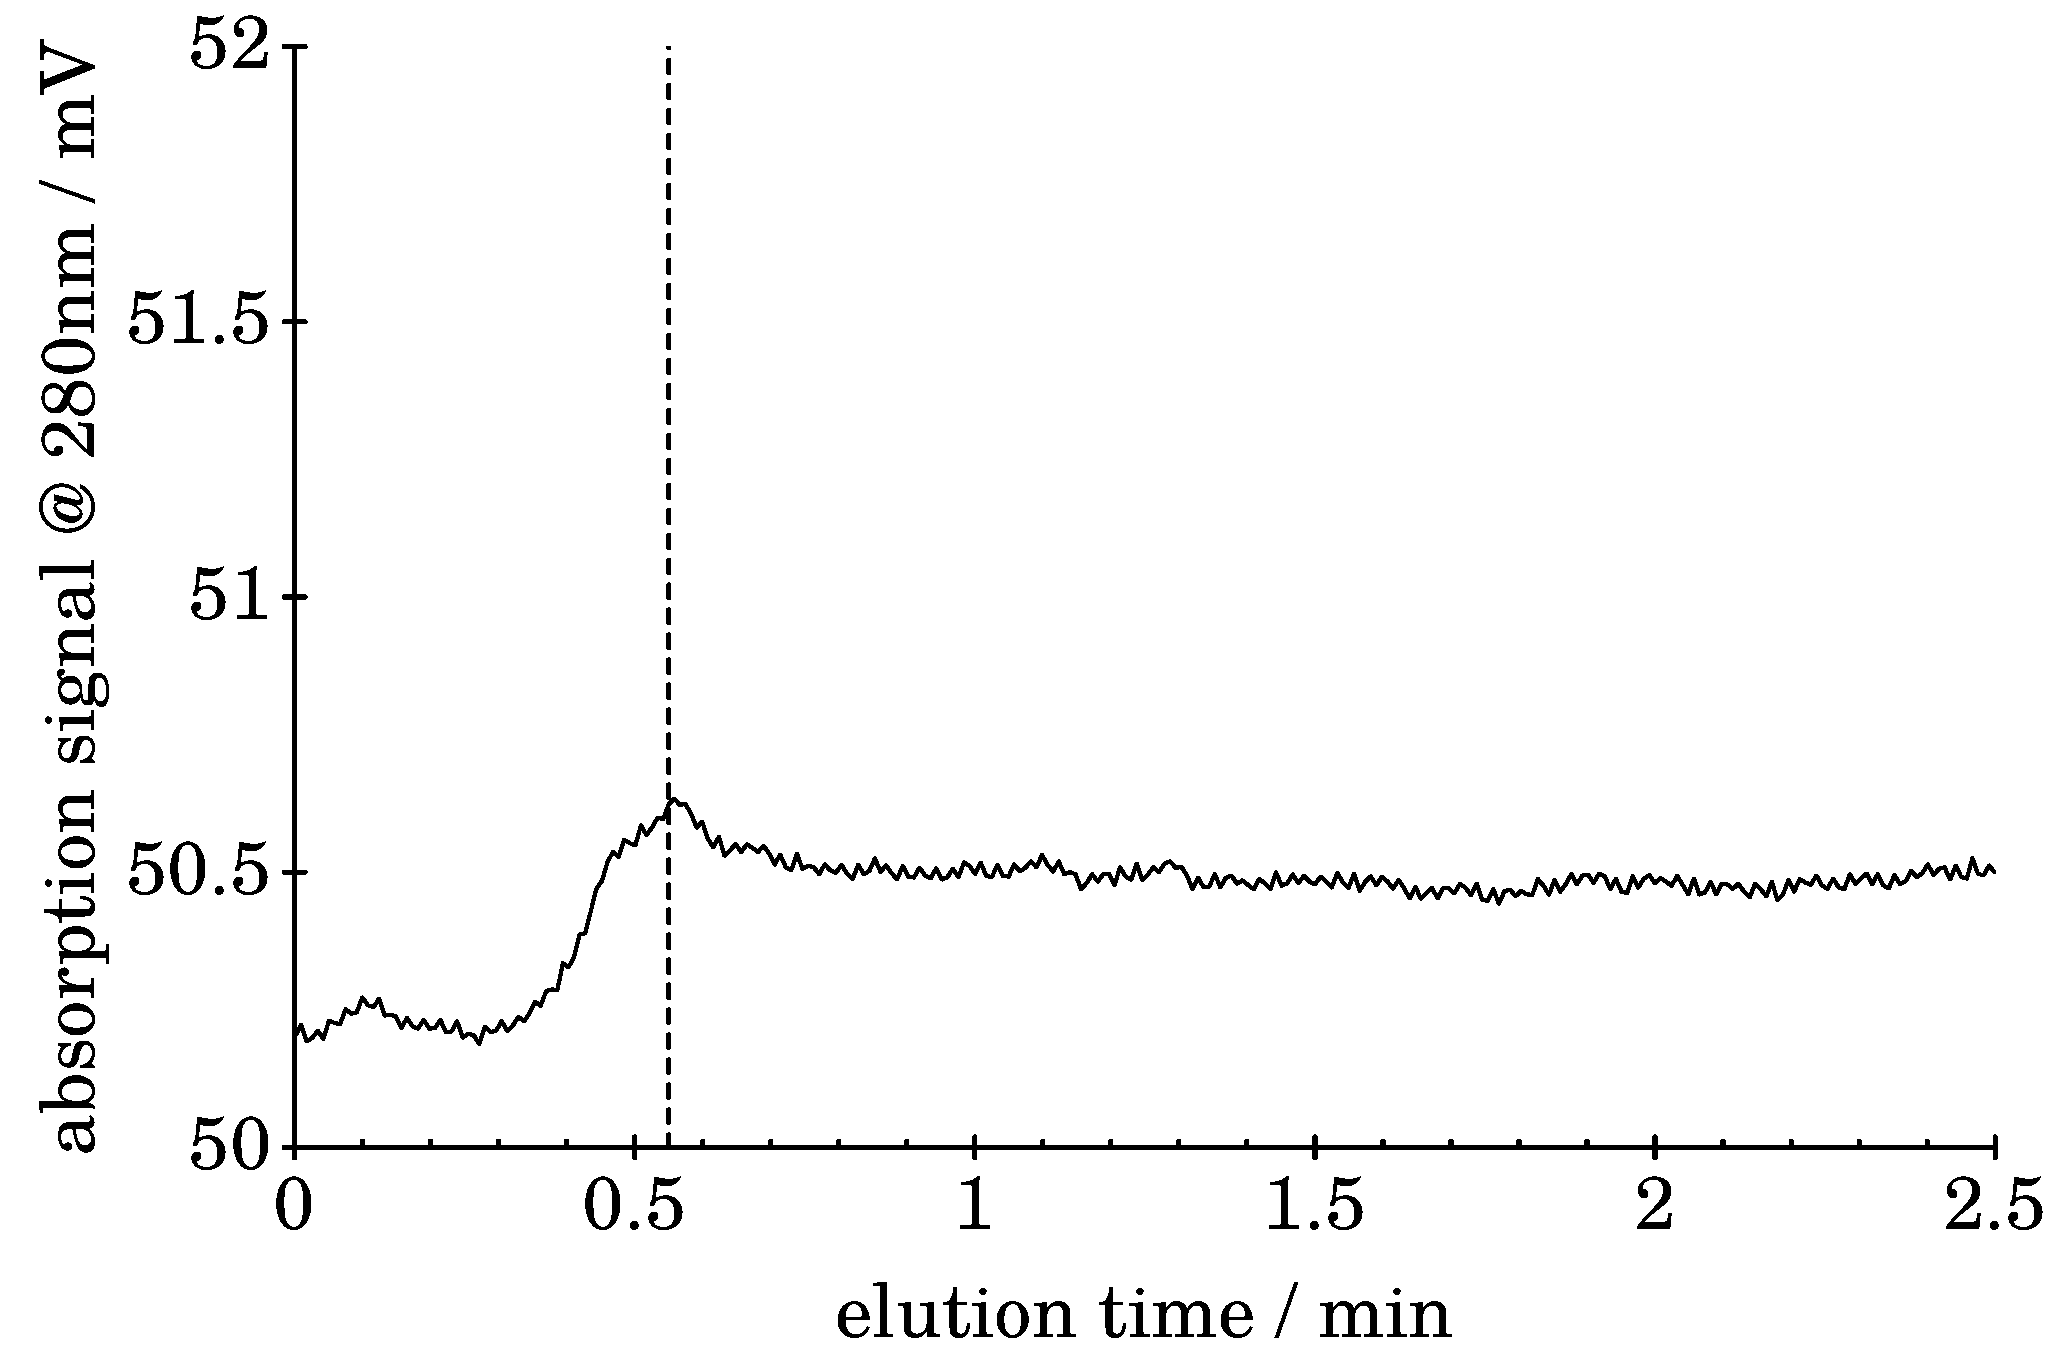
\includegraphics[width=\linewidth]{./images/data/rawPlots/img_BSA_VC_2_5_r2_t0.pdf}
    \subcaption{Detailed starting section of fractogram \ref{subfig:raw_BSA2_5_r2_te};
      Position of $\tvoid$, replicate 2.}
  \end{subfigure}
  \\\vspace*{.5em}
    %%%%%%%%%%%%%%%%%%%%%
  \begin{subfigure}{\subFigSize}
    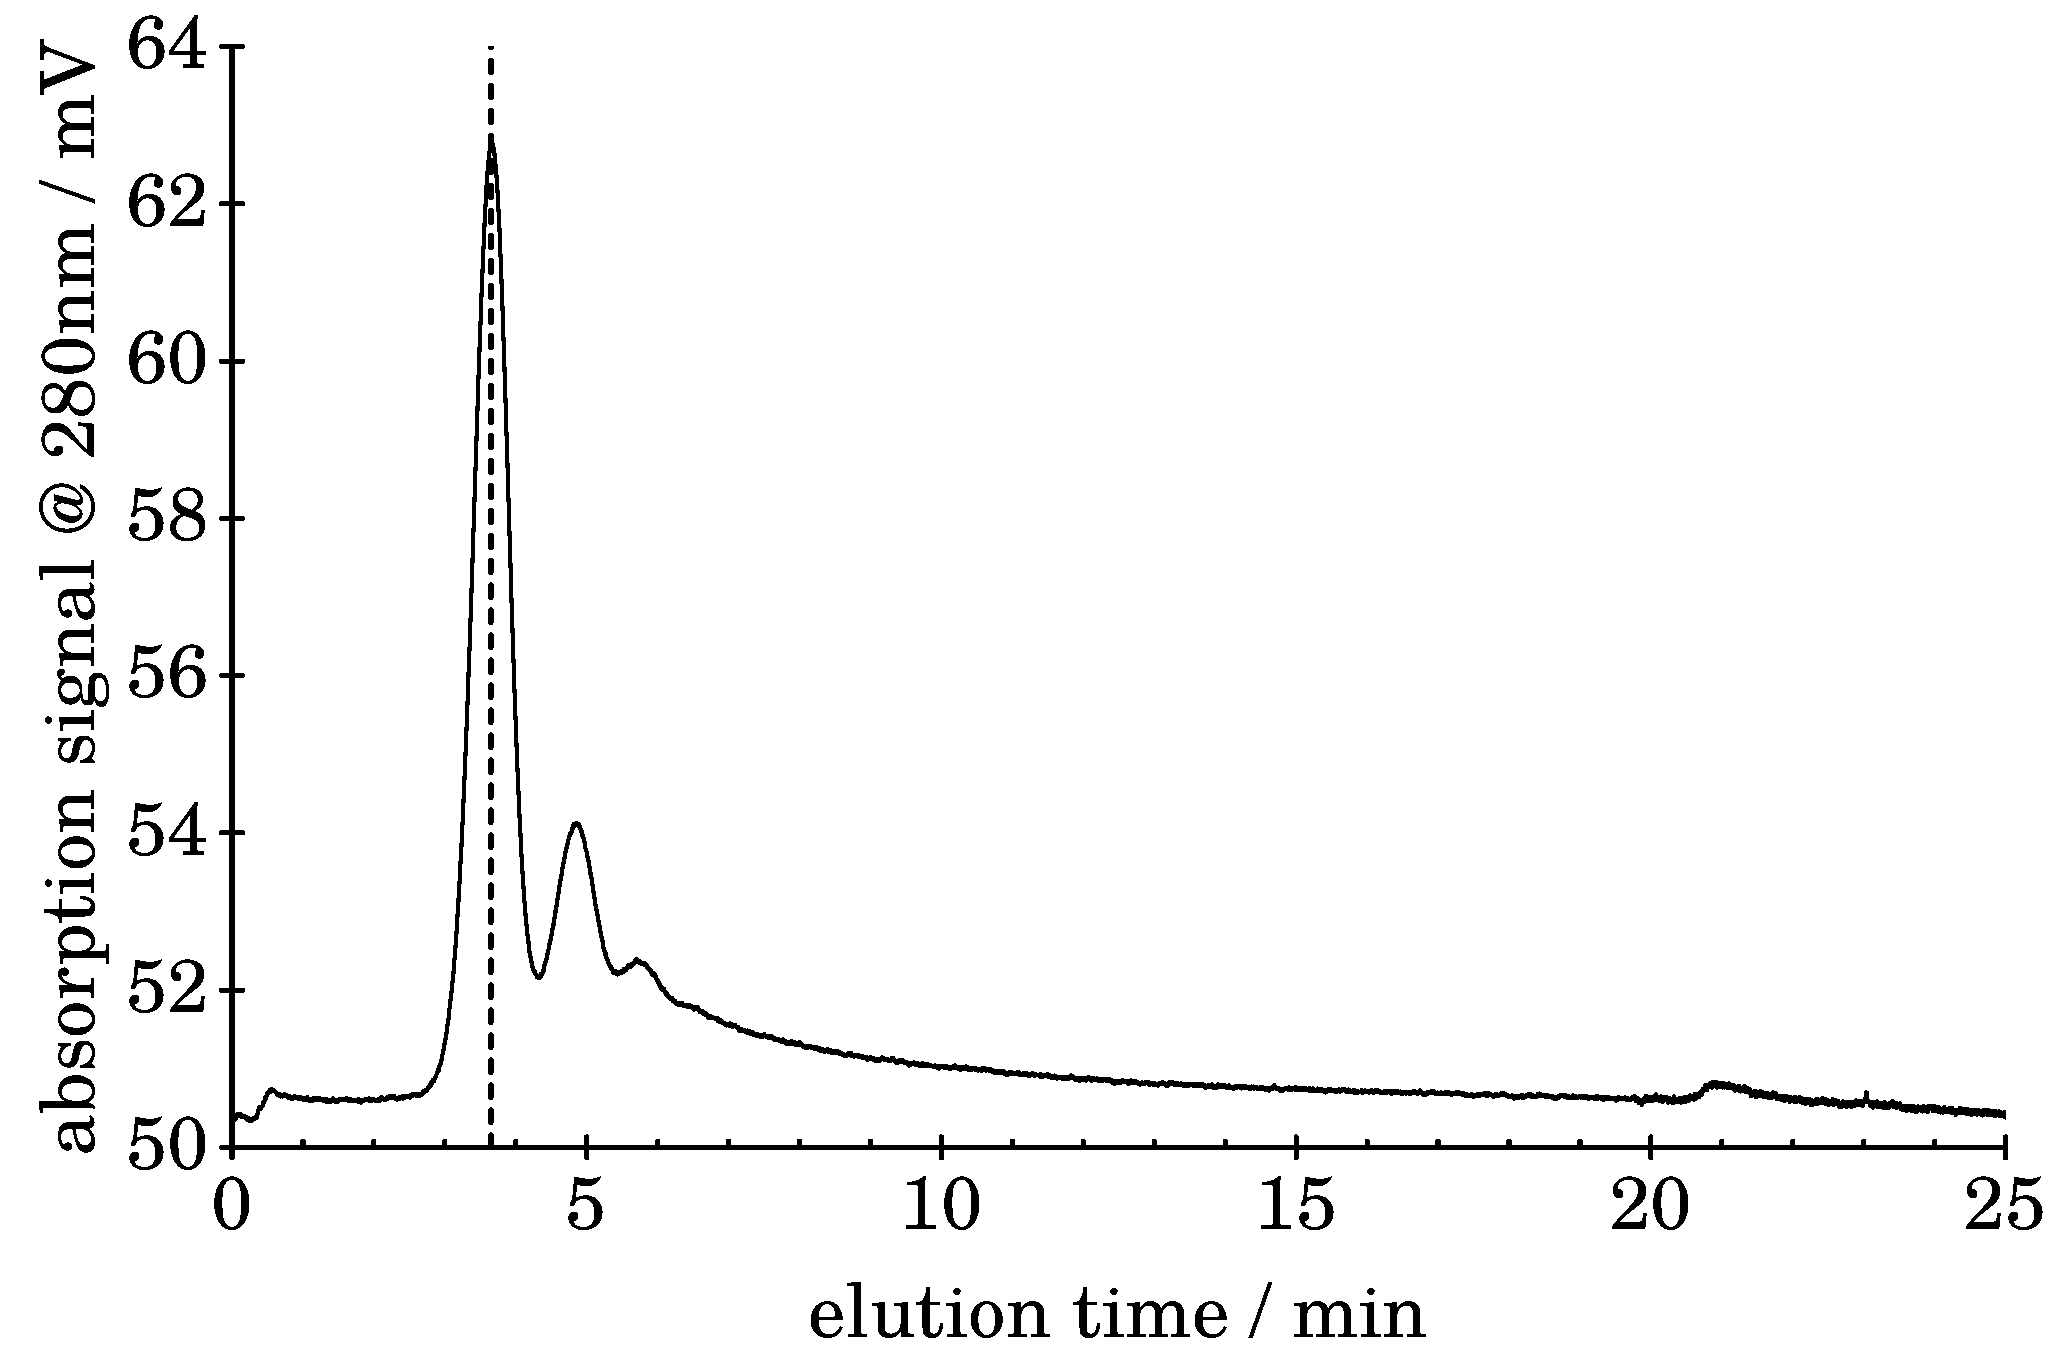
\includegraphics[width=\linewidth]{./images/data/rawPlots/img_BSA_VC_2_5_r3_te.pdf}
    \subcaption{Position of $\te$, replicate 3.}
    \label{subfig:raw_BSA2_5_r3_te}
  \end{subfigure}
  \begin{subfigure}{\subFigSize}
    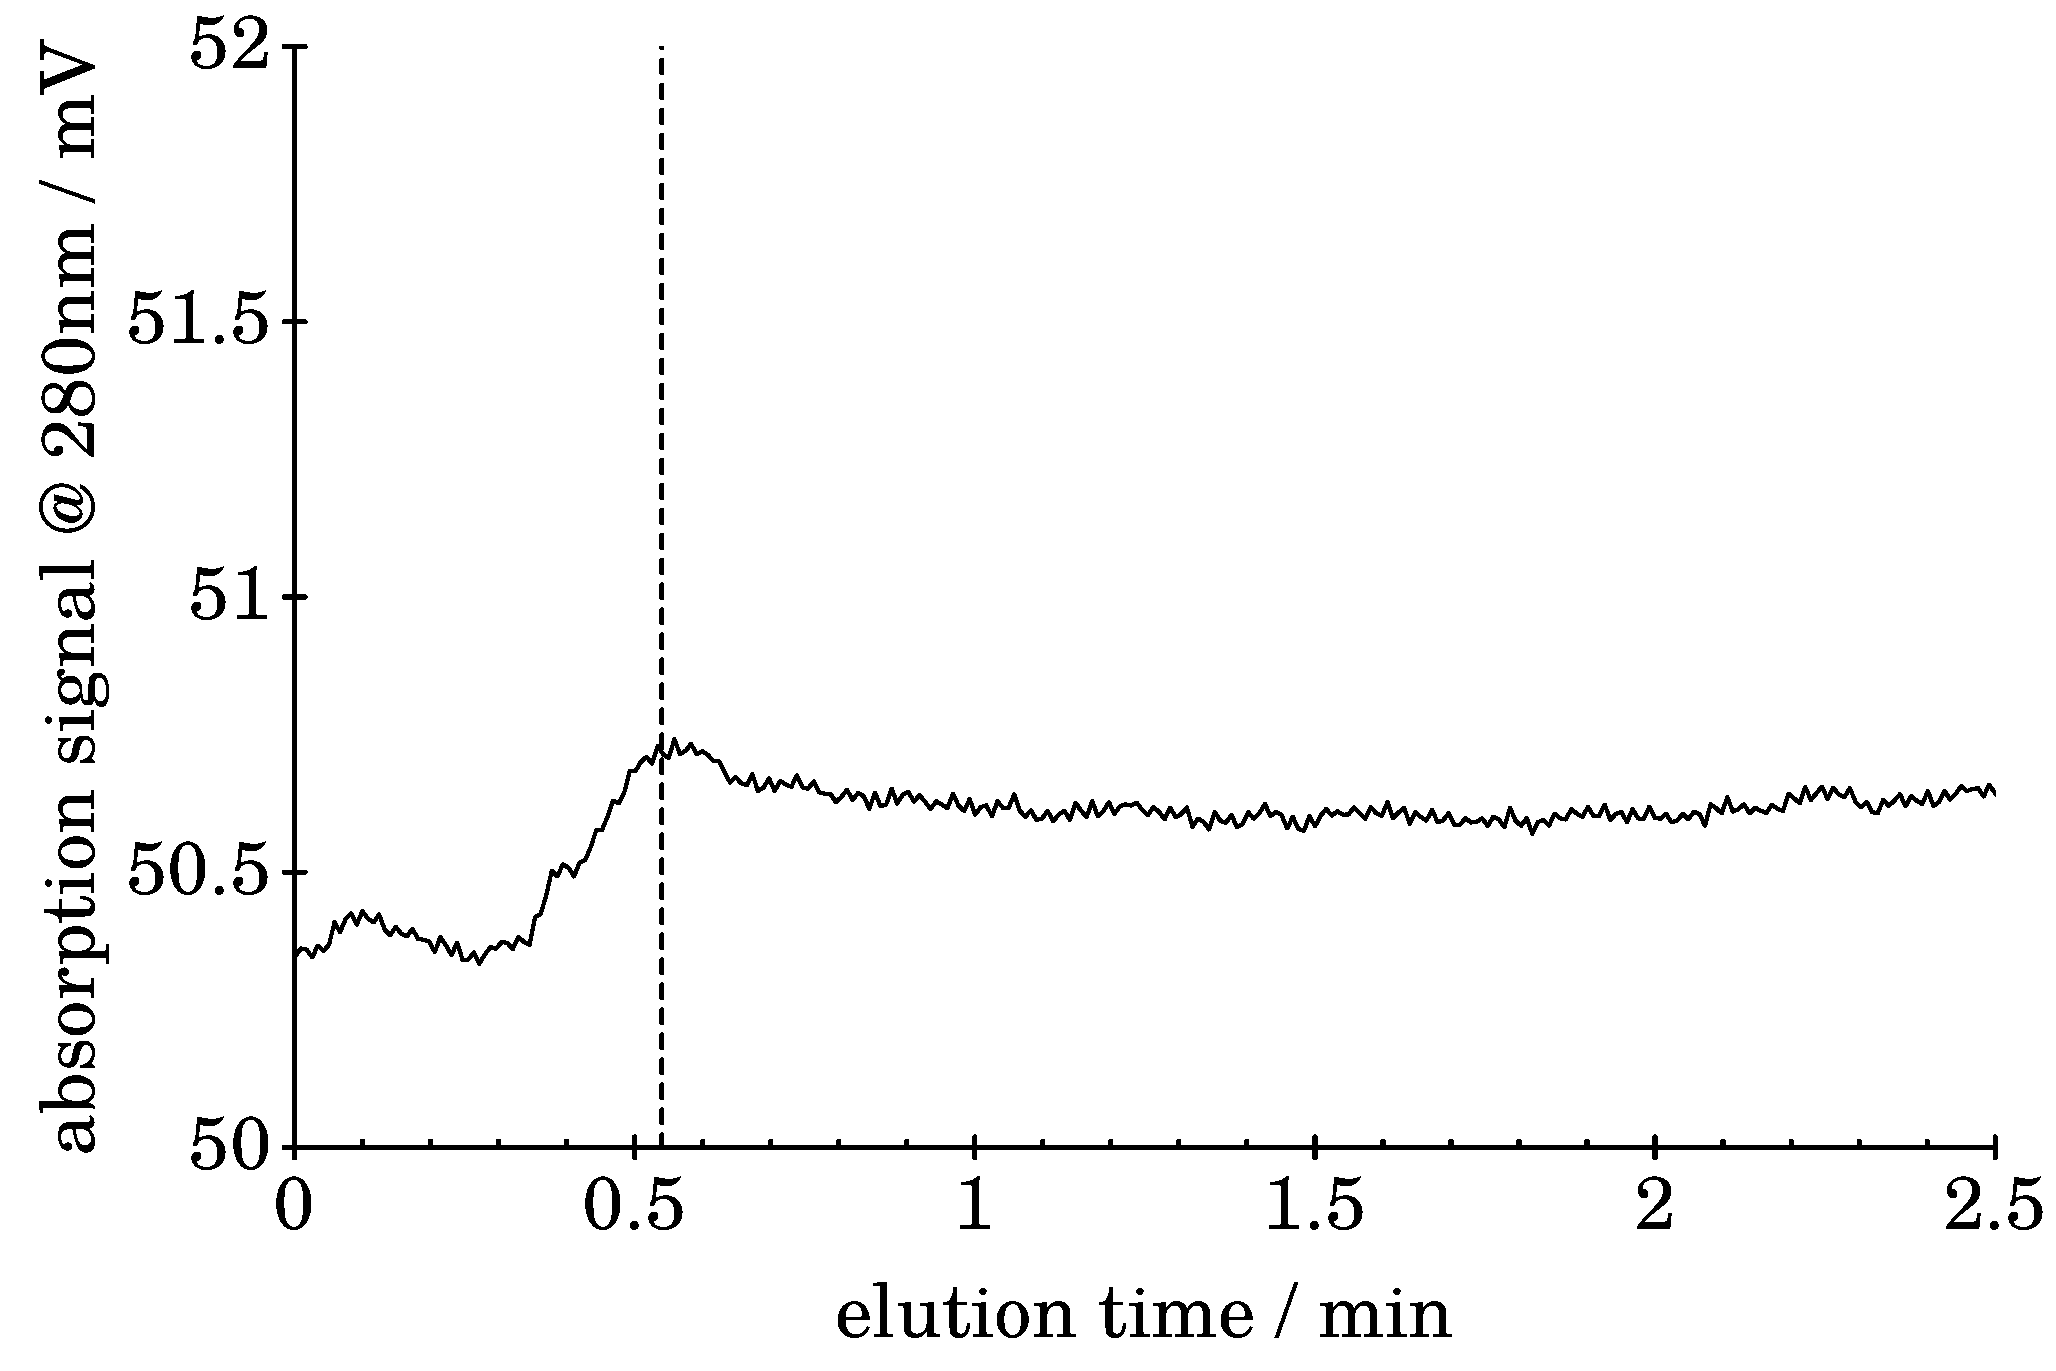
\includegraphics[width=\linewidth]{./images/data/rawPlots/img_BSA_VC_2_5_r3_t0.pdf}
    \subcaption{Detailed starting section of fractogram \ref{subfig:raw_BSA2_5_r3_te};
      Position of $\tvoid$, replicate 3.}
  \end{subfigure}
  \end{center}
  \vspace*{-3ex}    
  \caption[Raw fractograms of BSA measurements at $\Vc = \SI{2.5}{\mlmin}$]{Raw fractograms of BSA measurements at $\Vc 
  = \SI{2.5}{\mlmin}$}
  \label{fig:raw_BSA_2_5_UV} 
\end{figure}
\flushbottom
%%%%%%%%%%%%%%%%%%%%%%%%%%%%%%%%%%%%%%%%%%5
%%% BSA at Vc = 3.5 ml/min
%%%%%%%%%%%%%%%%%%%%%%%%%%%%%%%%%%%%%%%%
\begin{figure}[H]
  \begin{center}
    \begin{subfigure}{\subFigSize}
      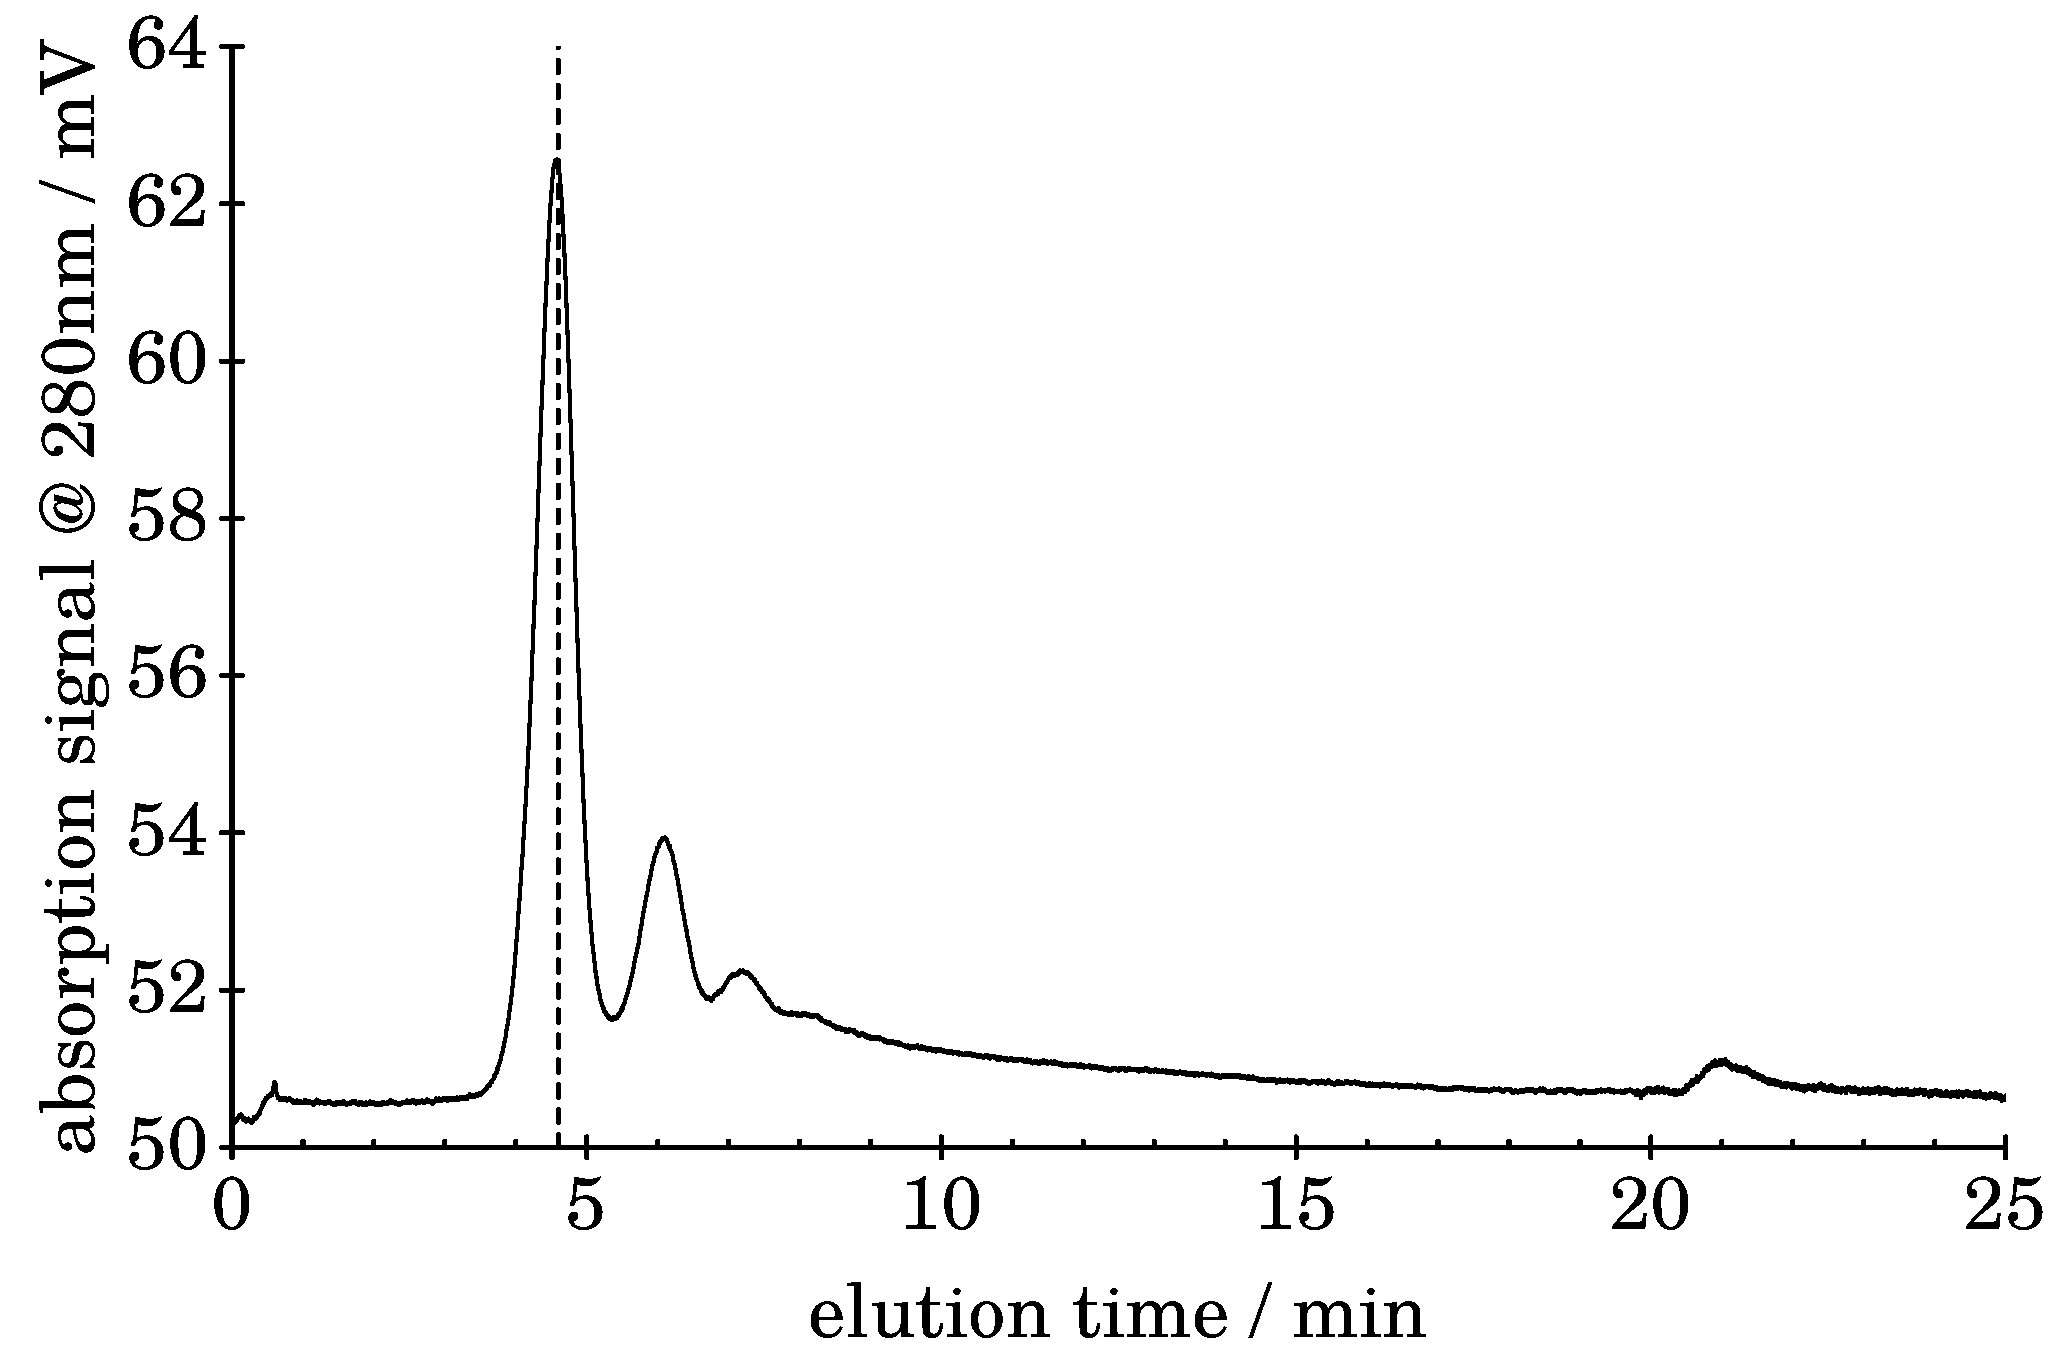
\includegraphics[width=\linewidth]{./images/data/rawPlots/img_BSA_VC_3_5_r1_te.pdf}
      \subcaption{Position of $\te$, replicate 1.}
      \label{subfig:raw_BSA3_5_r1_te}
    \end{subfigure}
    \begin{subfigure}{\subFigSize}
      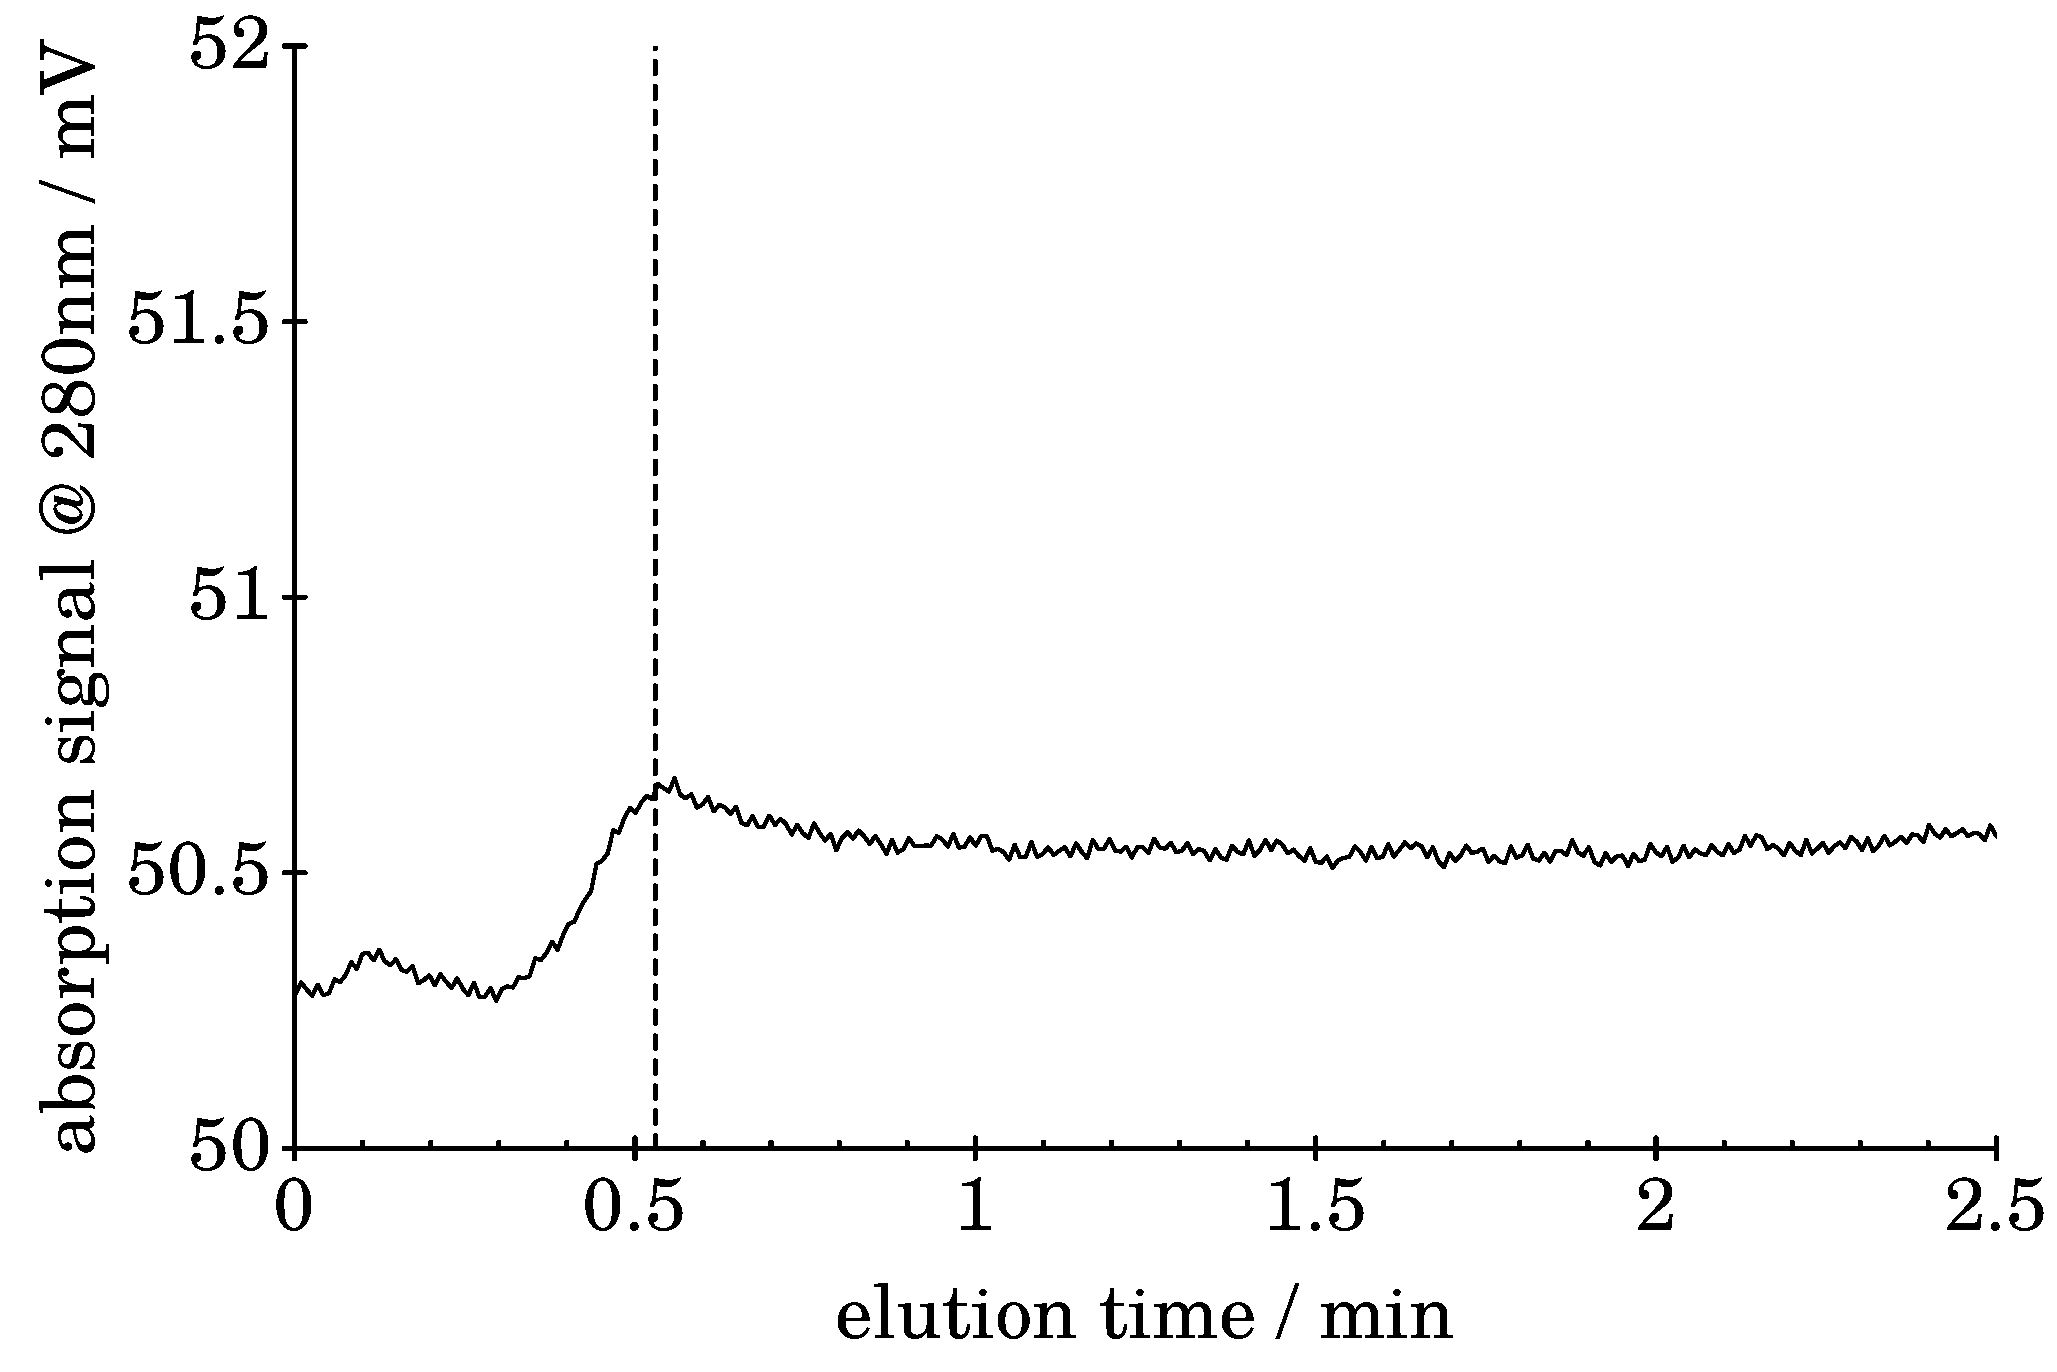
\includegraphics[width=\linewidth]{./images/data/rawPlots/img_BSA_VC_2_5_r1_t0.pdf}
      \subcaption{Detailed starting section of fractogram \ref{subfig:raw_BSA3_5_r1_te};
        Position of $\tvoid$, replicate 1.}
    \end{subfigure}
    \\\vspace*{.5em}
    %%%%%%%%%%%%%%%%%%%%%
    \begin{subfigure}{\subFigSize}
      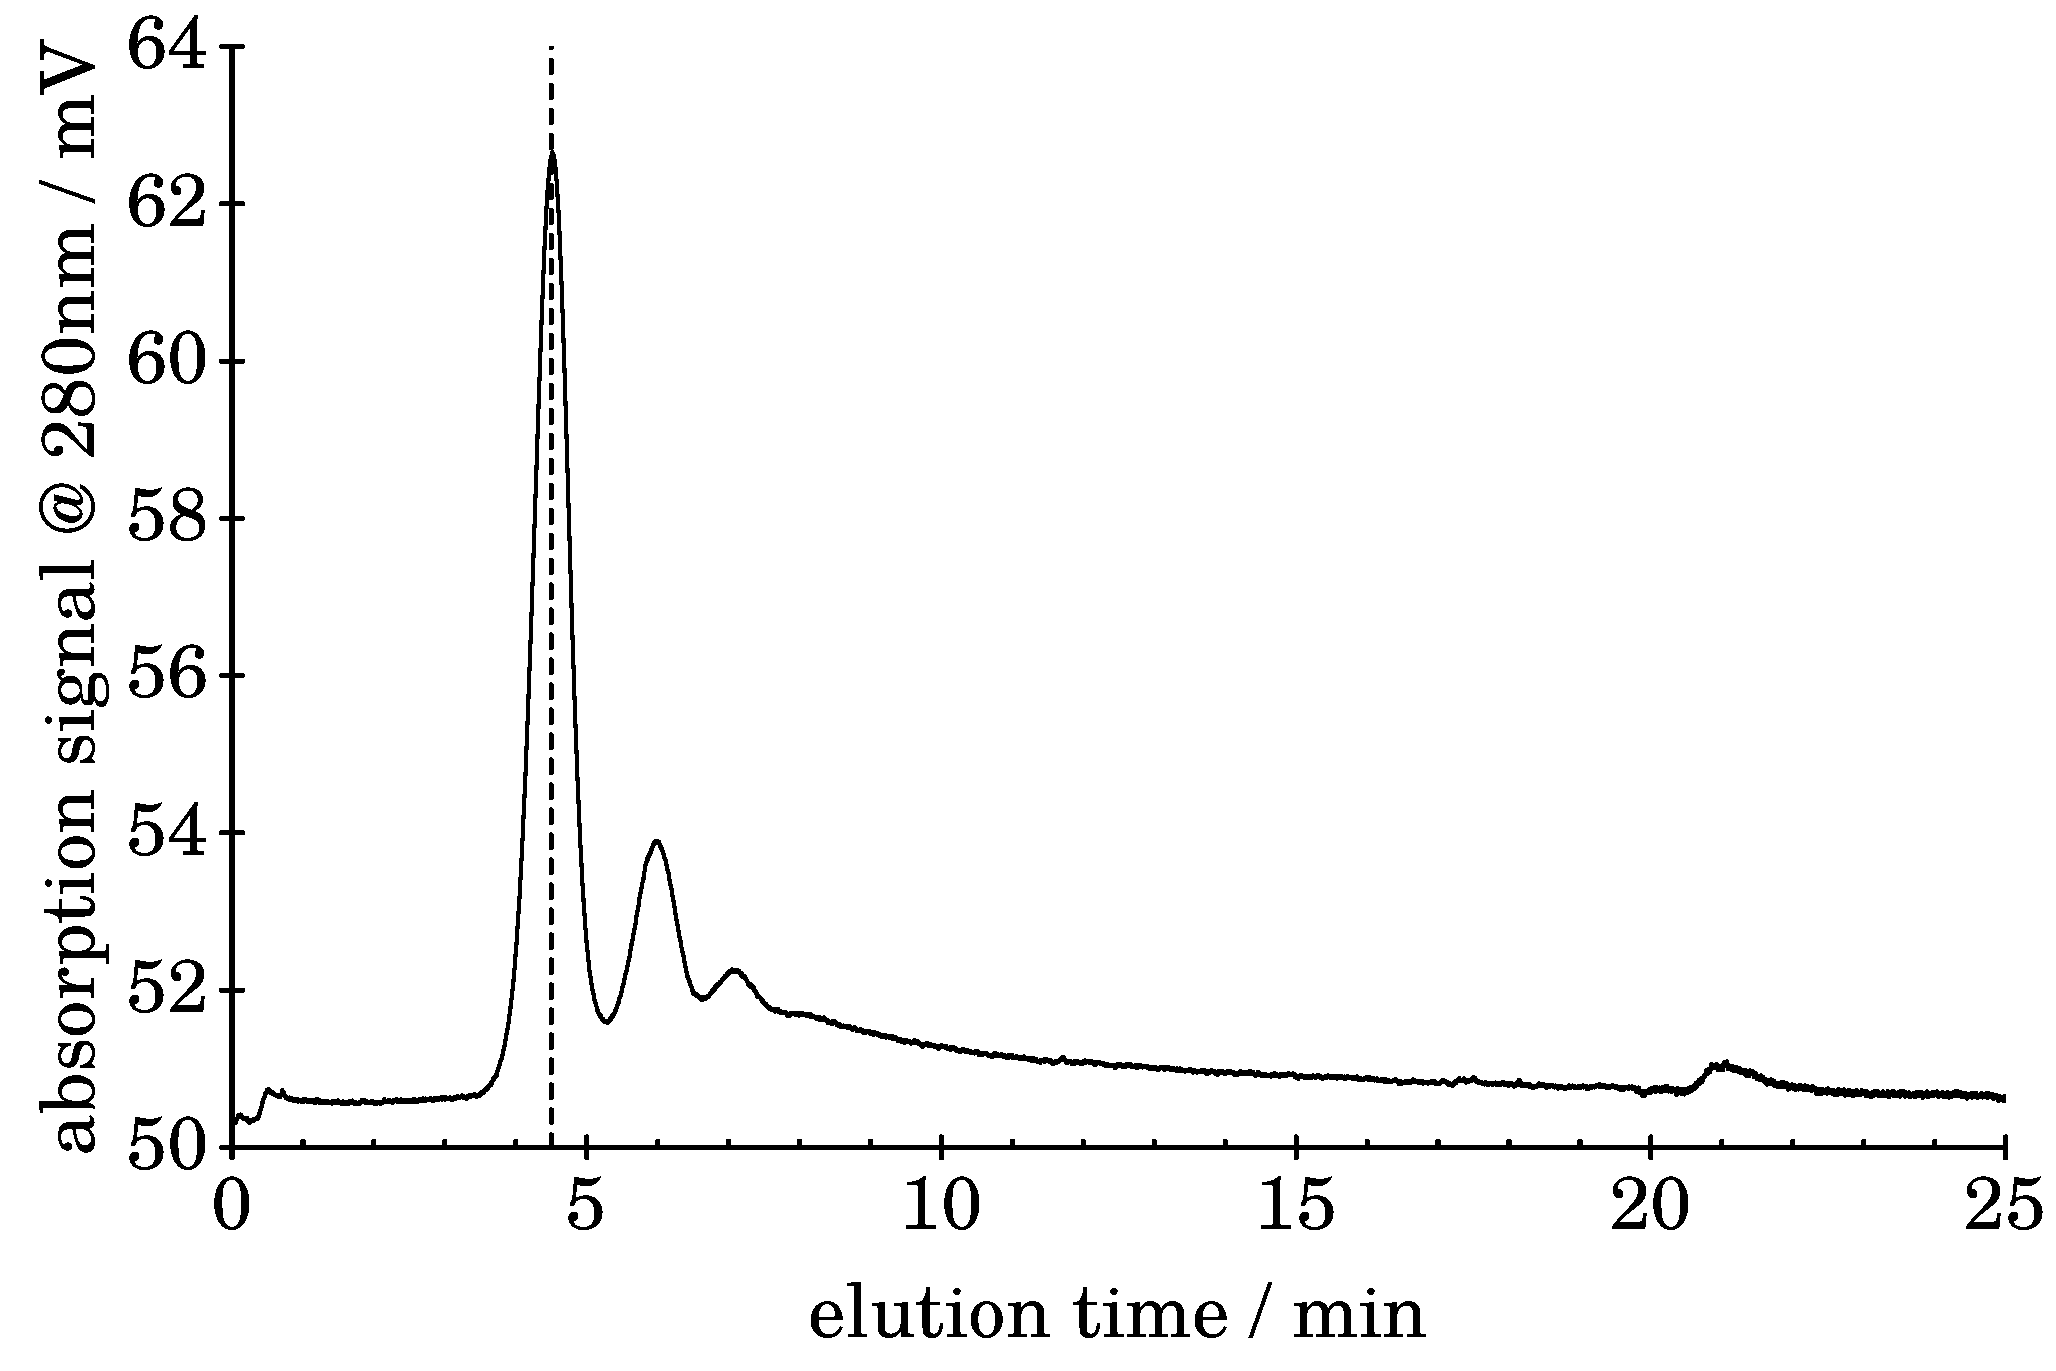
\includegraphics[width=\linewidth]{./images/data/rawPlots/img_BSA_VC_3_5_r2_te.pdf}
      \subcaption{Position of $\te$, replicate 2.}
      \label{subfig:raw_BSA3_5_r2_te}
    \end{subfigure}
    \begin{subfigure}{\subFigSize}
      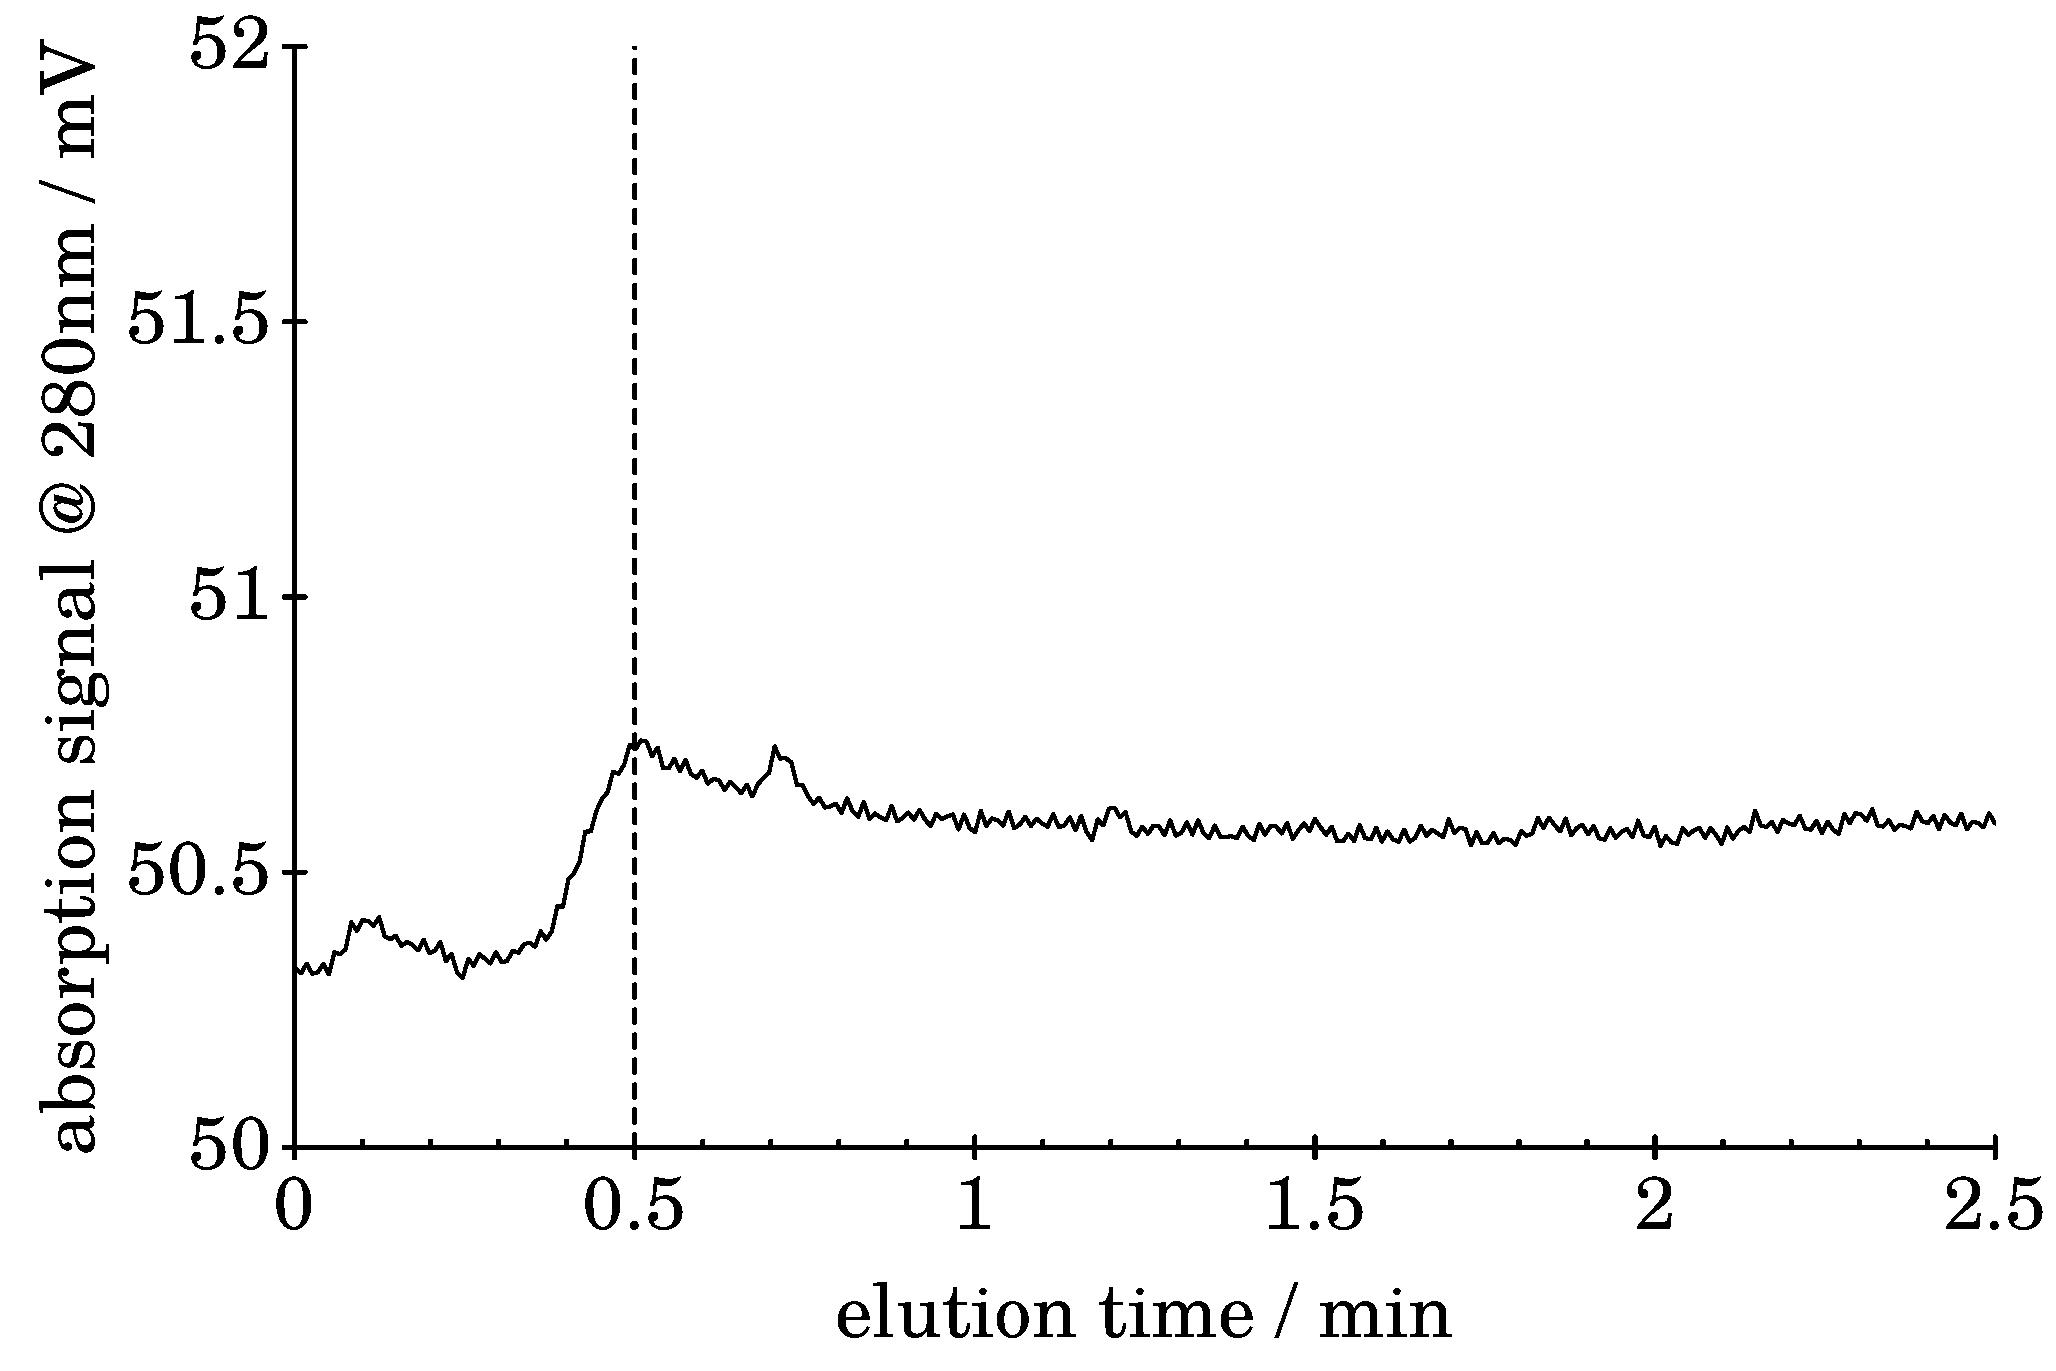
\includegraphics[width=\linewidth]{./images/data/rawPlots/img_BSA_VC_3_5_r2_t0.pdf}
      \subcaption{Detailed starting section of fractogram \ref{subfig:raw_BSA3_5_r2_te};
        Position of $\tvoid$, replicate 2.}
    \end{subfigure}
    \\\vspace*{.5em}
    %%%%%%%%%%%%%%%%%%%%%
    \begin{subfigure}{\subFigSize}
      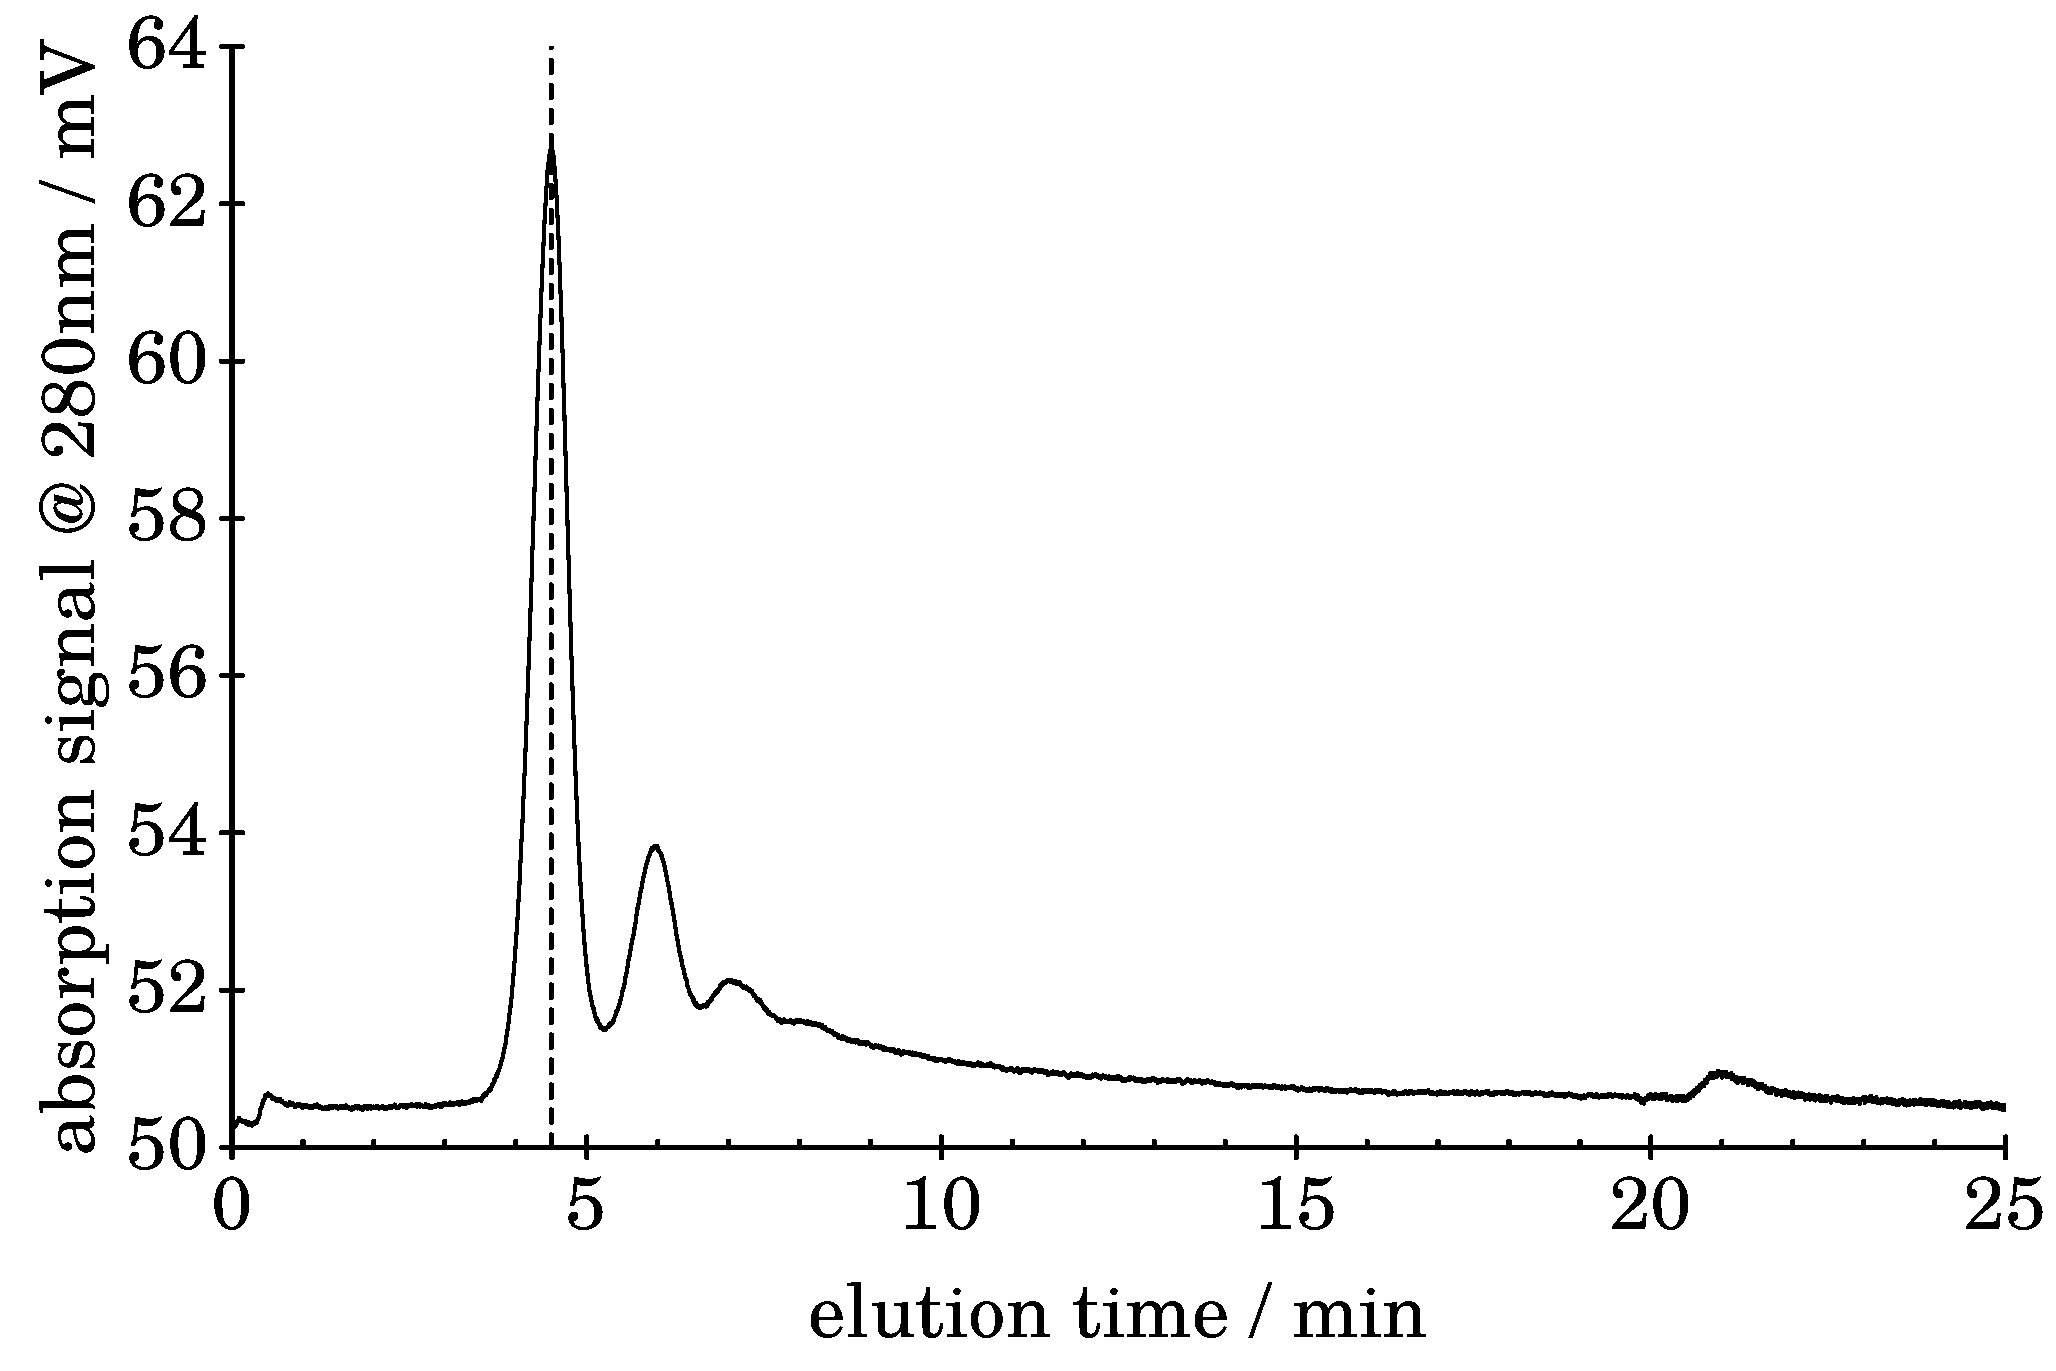
\includegraphics[width=\linewidth]{./images/data/rawPlots/img_BSA_VC_3_5_r3_te.pdf}
      \subcaption{Position of $\te$, replicate 3.}
      \label{subfig:raw_BSA3_5_r3_te}
    \end{subfigure}
    \begin{subfigure}{\subFigSize}
      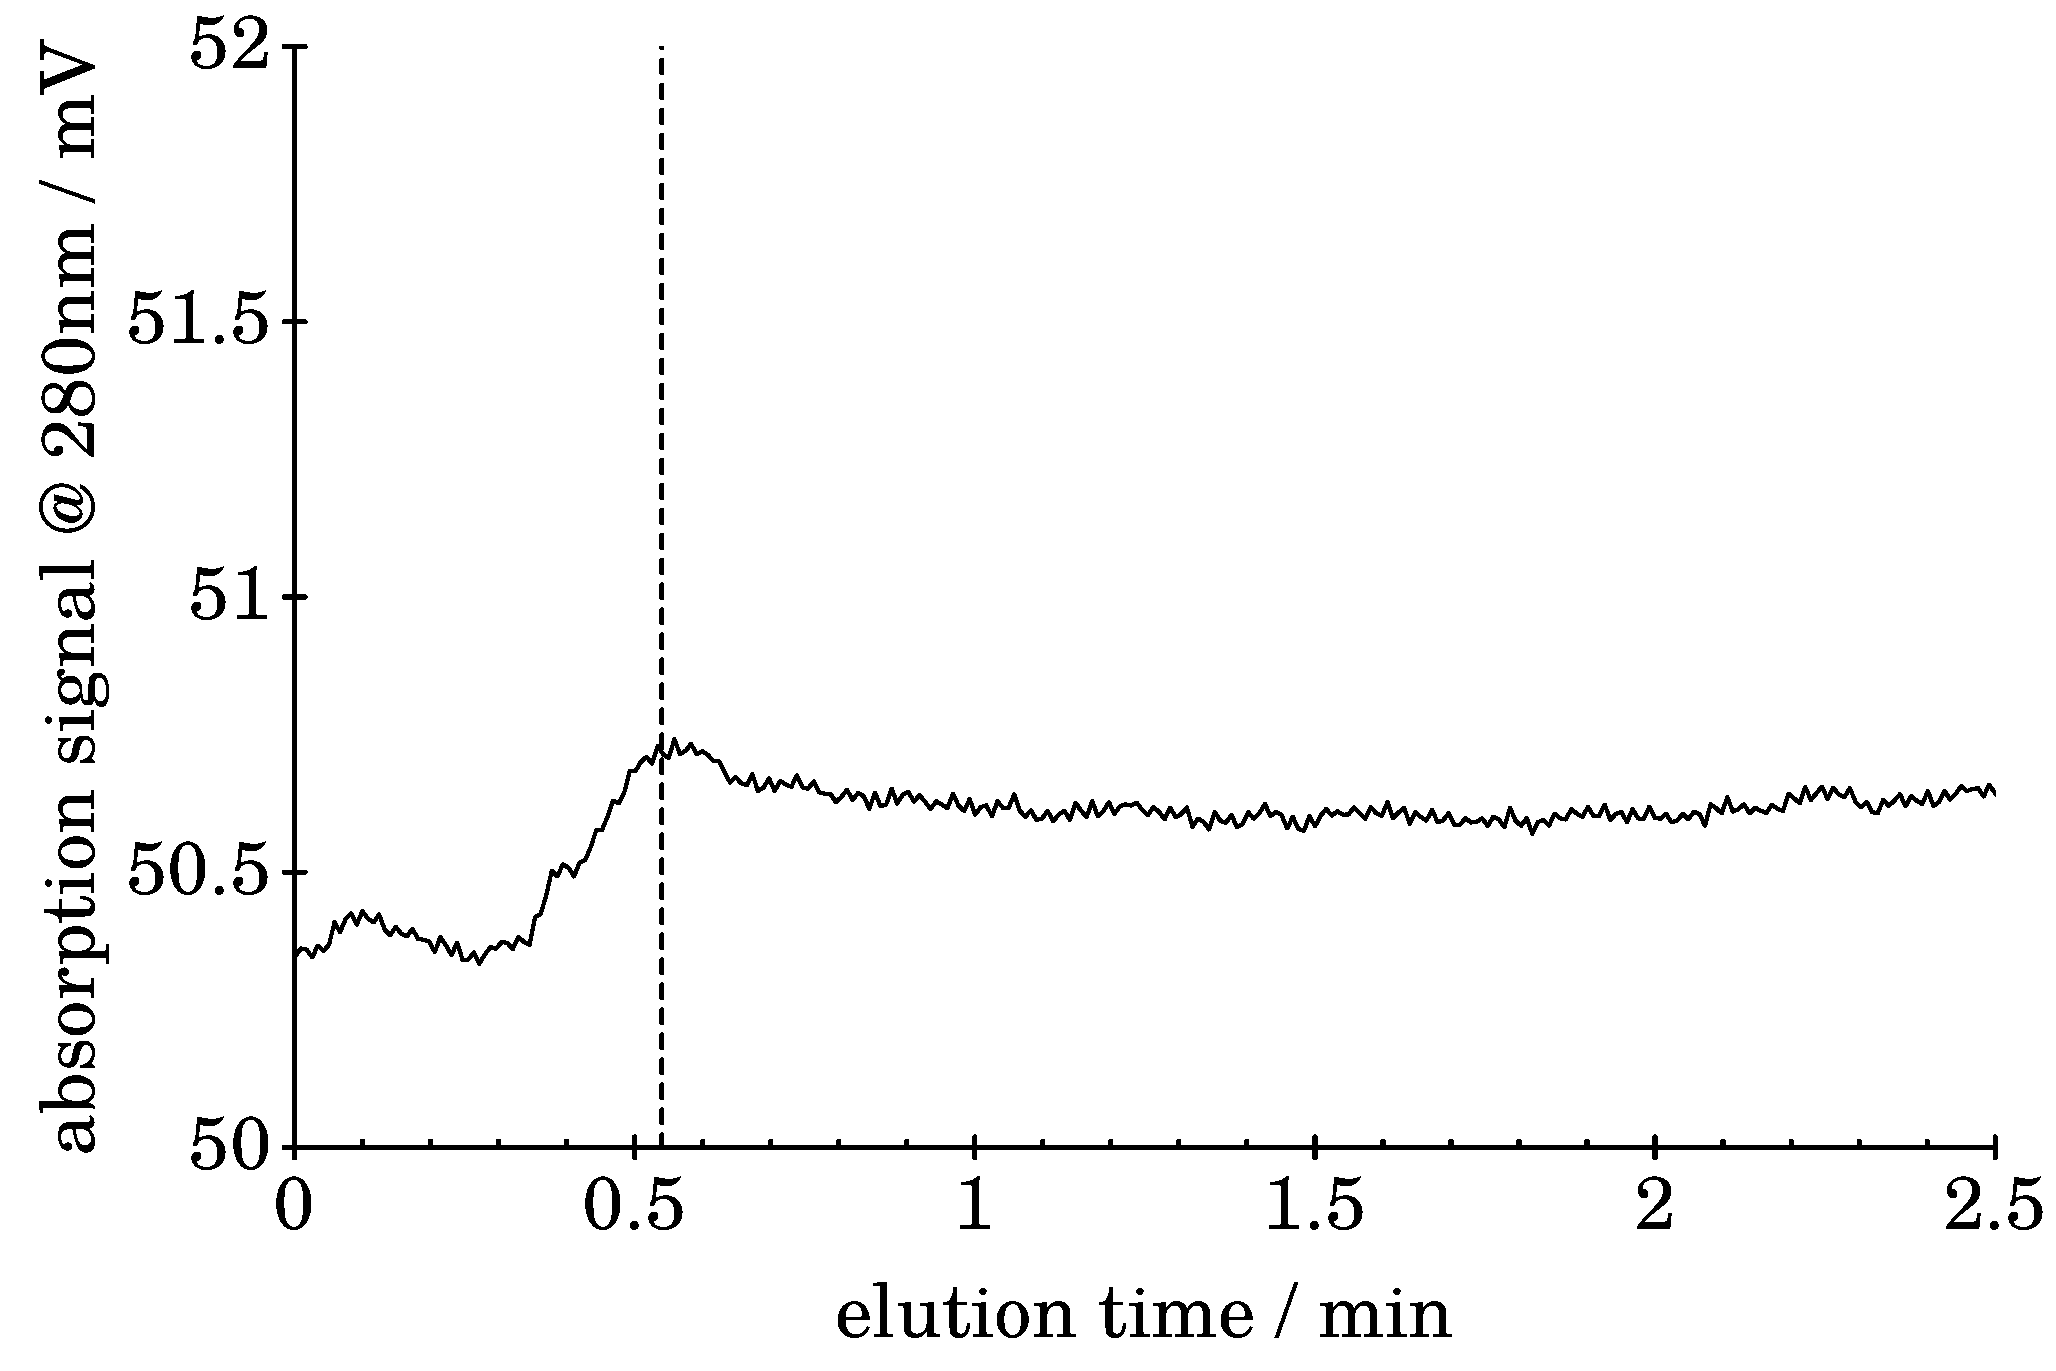
\includegraphics[width=\linewidth]{./images/data/rawPlots/img_BSA_VC_2_5_r3_t0.pdf}
      \subcaption{Detailed starting section of fractogram \ref{subfig:raw_BSA3_5_r3_te};
        Position of $\tvoid$, replicate 3.}
    \end{subfigure}
  \end{center}
  \vspace*{-3ex}    
  \caption[Raw fractograms of BSA measurements at $\Vc = \SI{3.5}{\mlmin}$]{Raw fractograms of BSA measurements at $\Vc 
  = \SI{3.5}{\mlmin}$}
  \label{fig:raw_BSA_3_5_UV} 
\end{figure}
\flushbottom
%%%%%%%%%%%%%%%%%%%%%%%%%%%%%%%%%%%%%%%%%%5
%%% PS at Vc = 0.5 ml/min, replicate 1
%%%%%%%%%%%%%%%%%%%%%%%%%%%%%%%%%%%%%%%%
\begin{figure}[t!]
  \begin{center}
    \begin{subfigure}{\subFigSize}
      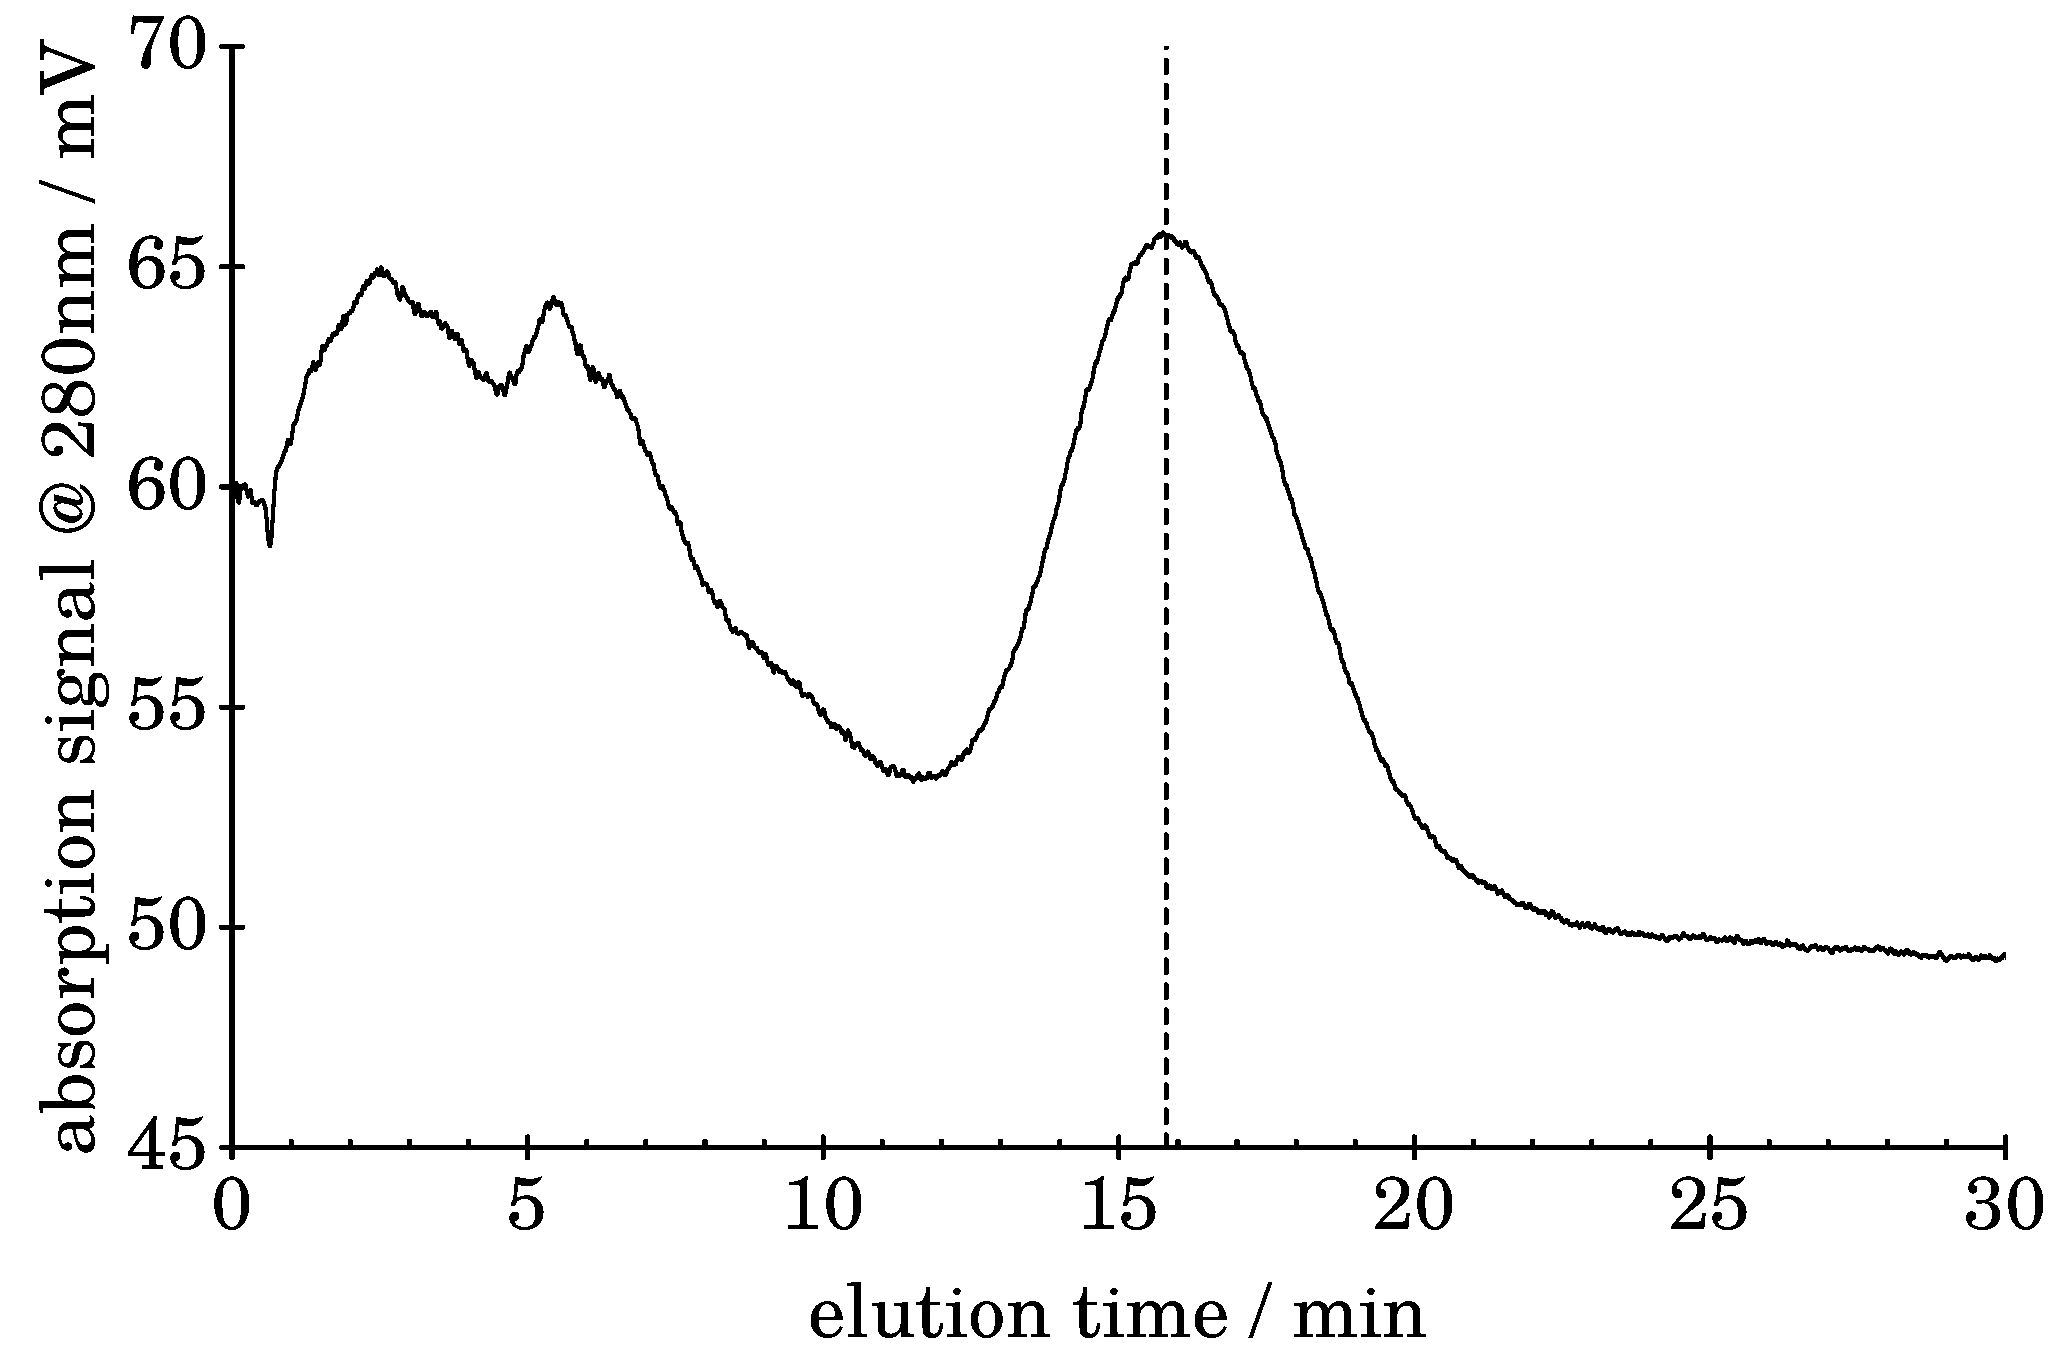
\includegraphics[width=\linewidth]{./images/data/rawPlots/img_PS_VC_05_rep1_te_UV.pdf}
      \subcaption{Position of $\te$ with UV detection signal}
      \label{subfig:raw_PS2_5_r1_te_UV}
    \end{subfigure}
    \begin{subfigure}{\subFigSize}
      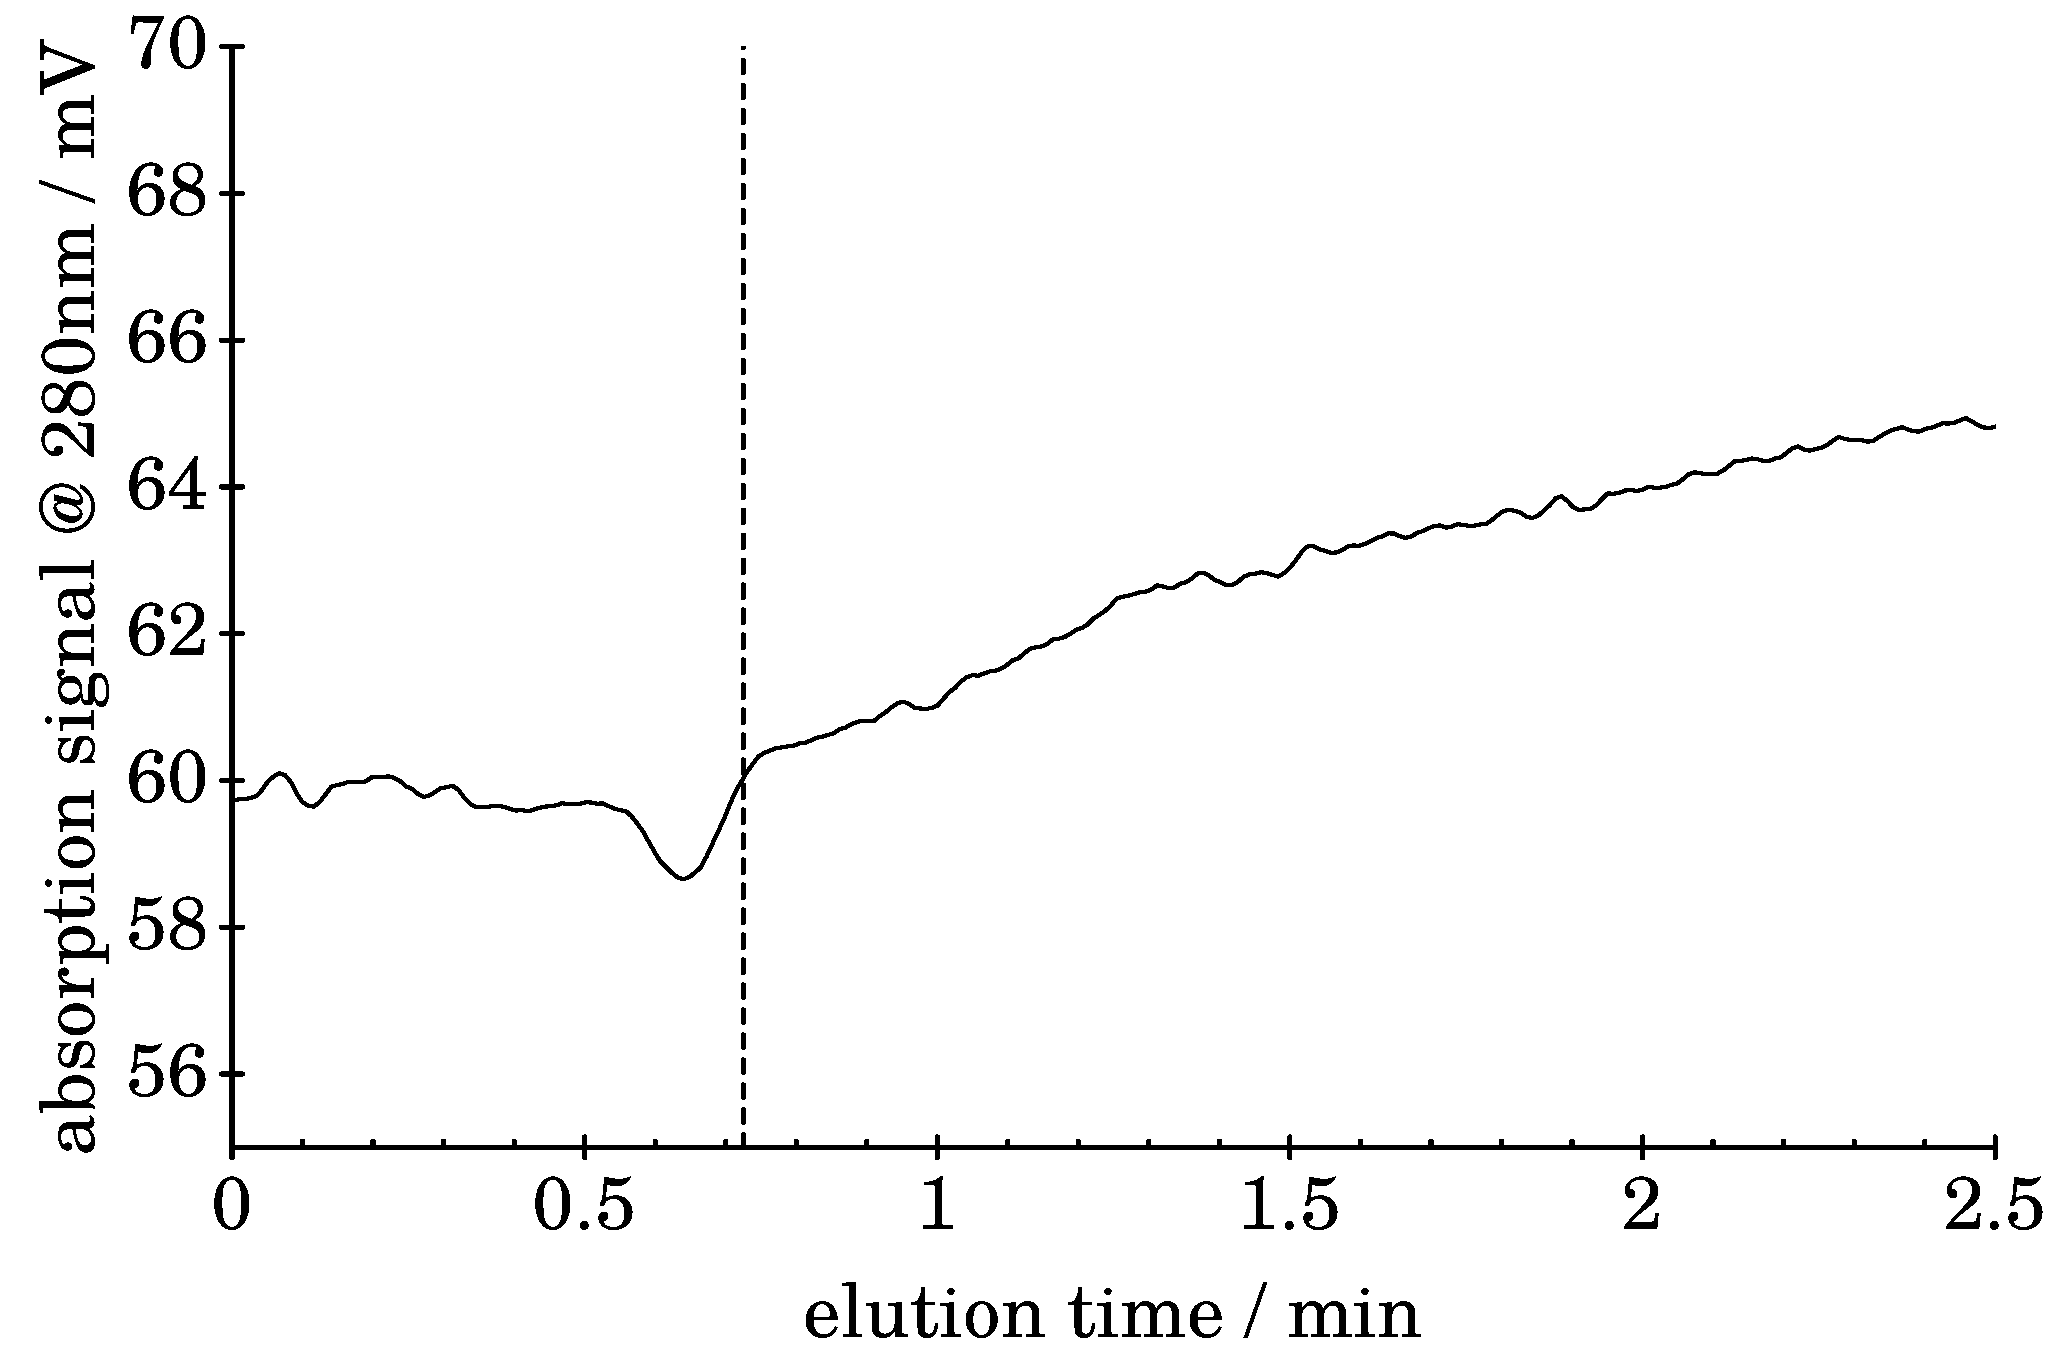
\includegraphics[width=\linewidth]{./images/data/rawPlots/img_PS_VC_05_rep1_t0_UV.pdf}
      \subcaption{Detailed starting section of fractogram \ref{subfig:raw_PS2_5_r1_te_UV}
         with UV detection signal and position of $\tvoid$.}
    \end{subfigure}
  %%%%%%%%%%%%%%%%%%
    \\\vspace*{.5em}
  %%%%%%%%%%%%%%
  \begin{subfigure}{\subFigSize} 
    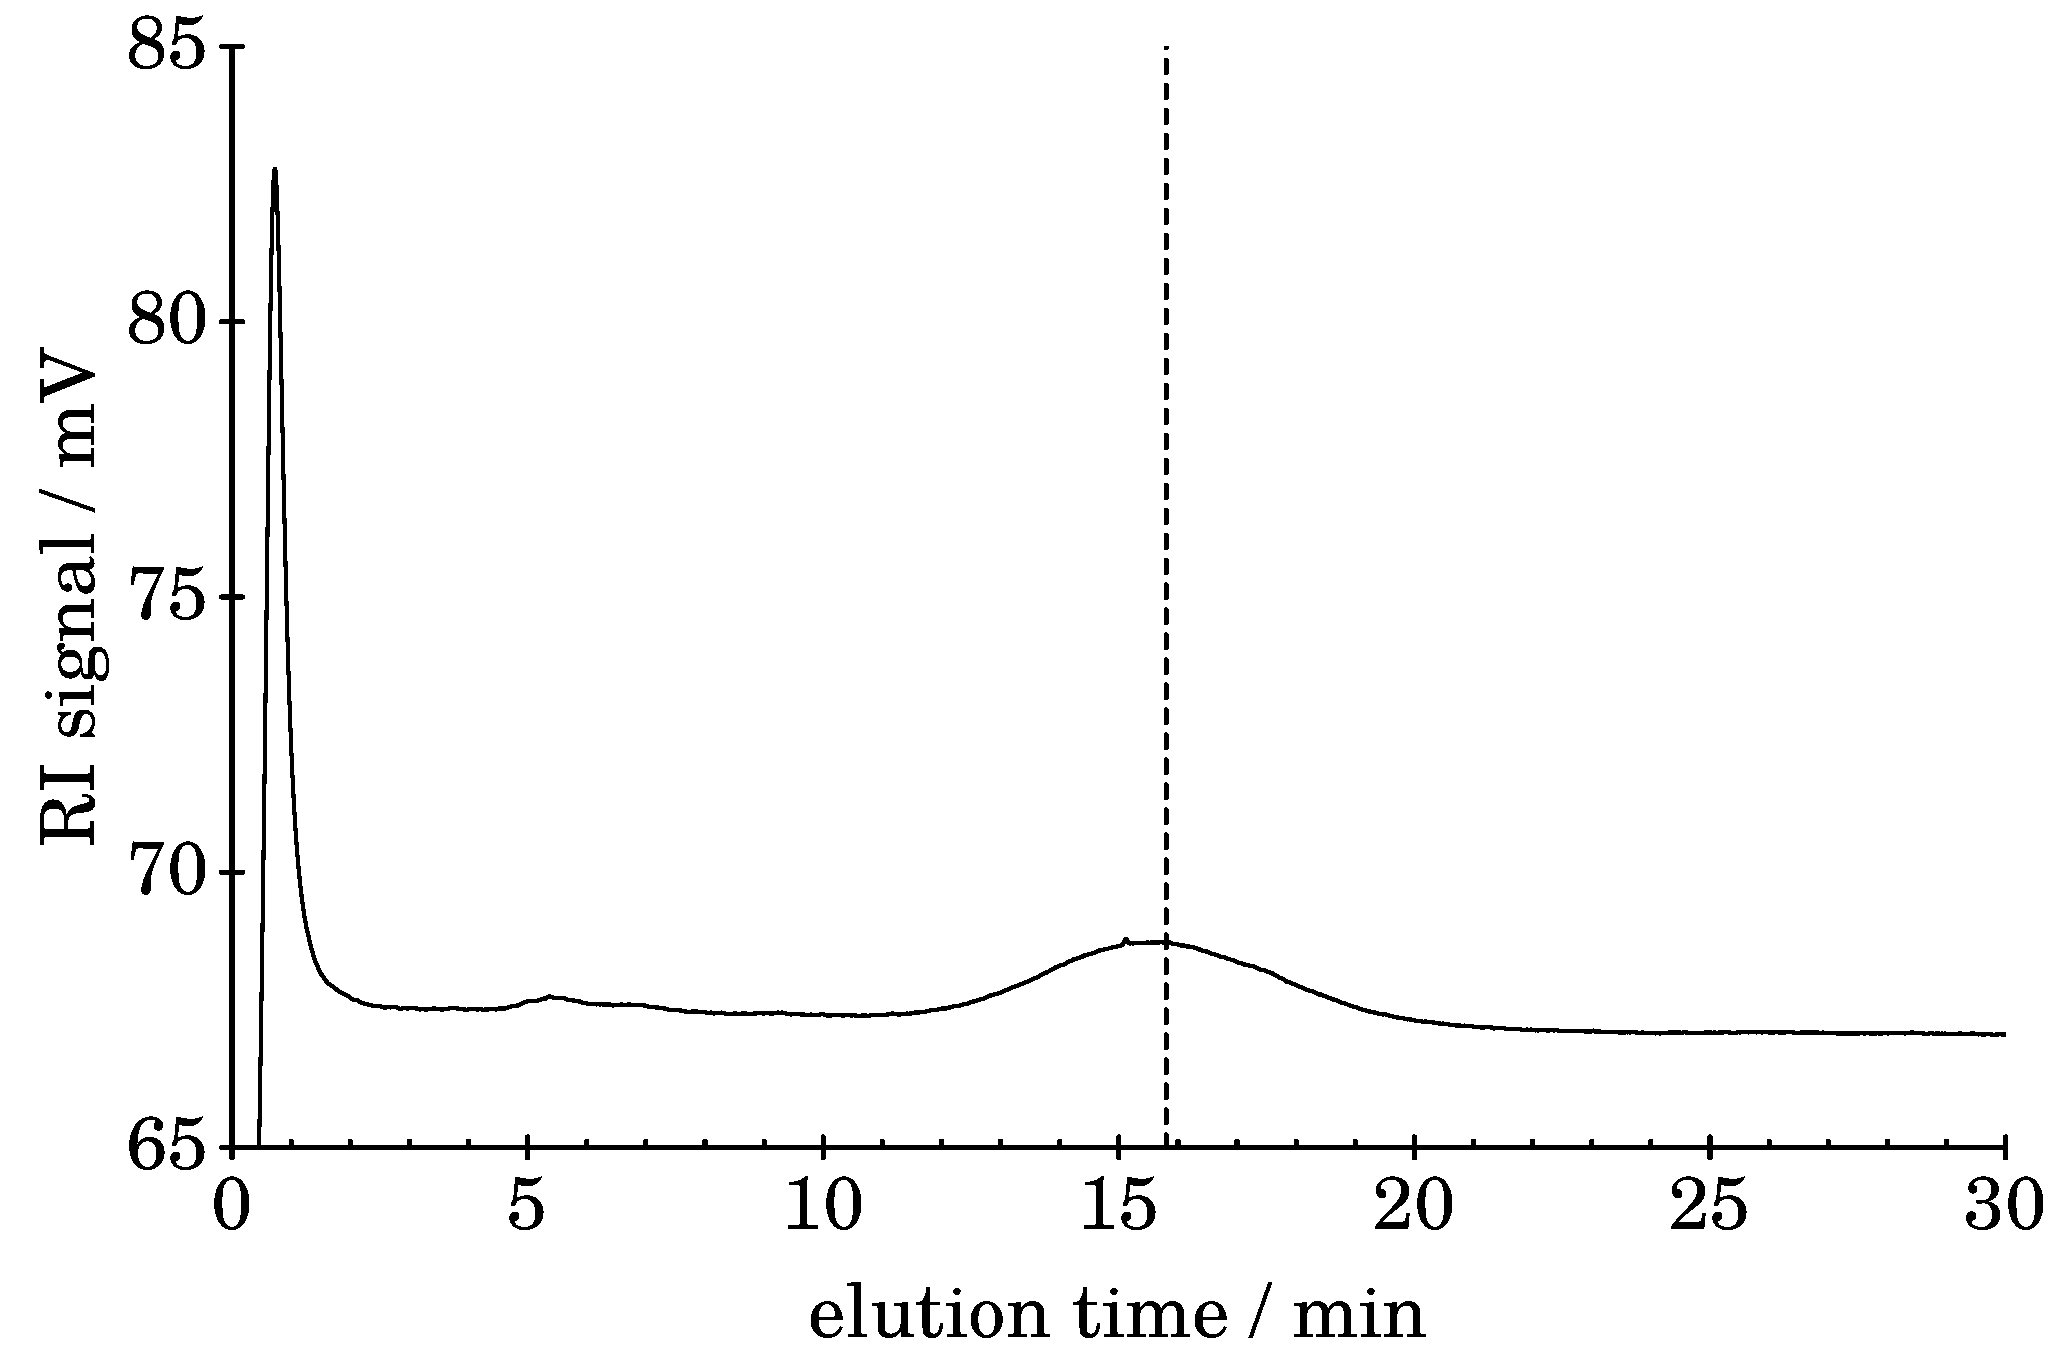
\includegraphics[width=\linewidth]{./images/data/rawPlots/img_PS_VC_05_rep1_te_RI.pdf}
    \subcaption{Position of $\te$ with RI detection signal}
    \label{subfig:raw_PS2_5_r1_te_RI}
  \end{subfigure}
  \begin{subfigure}{\subFigSize}
    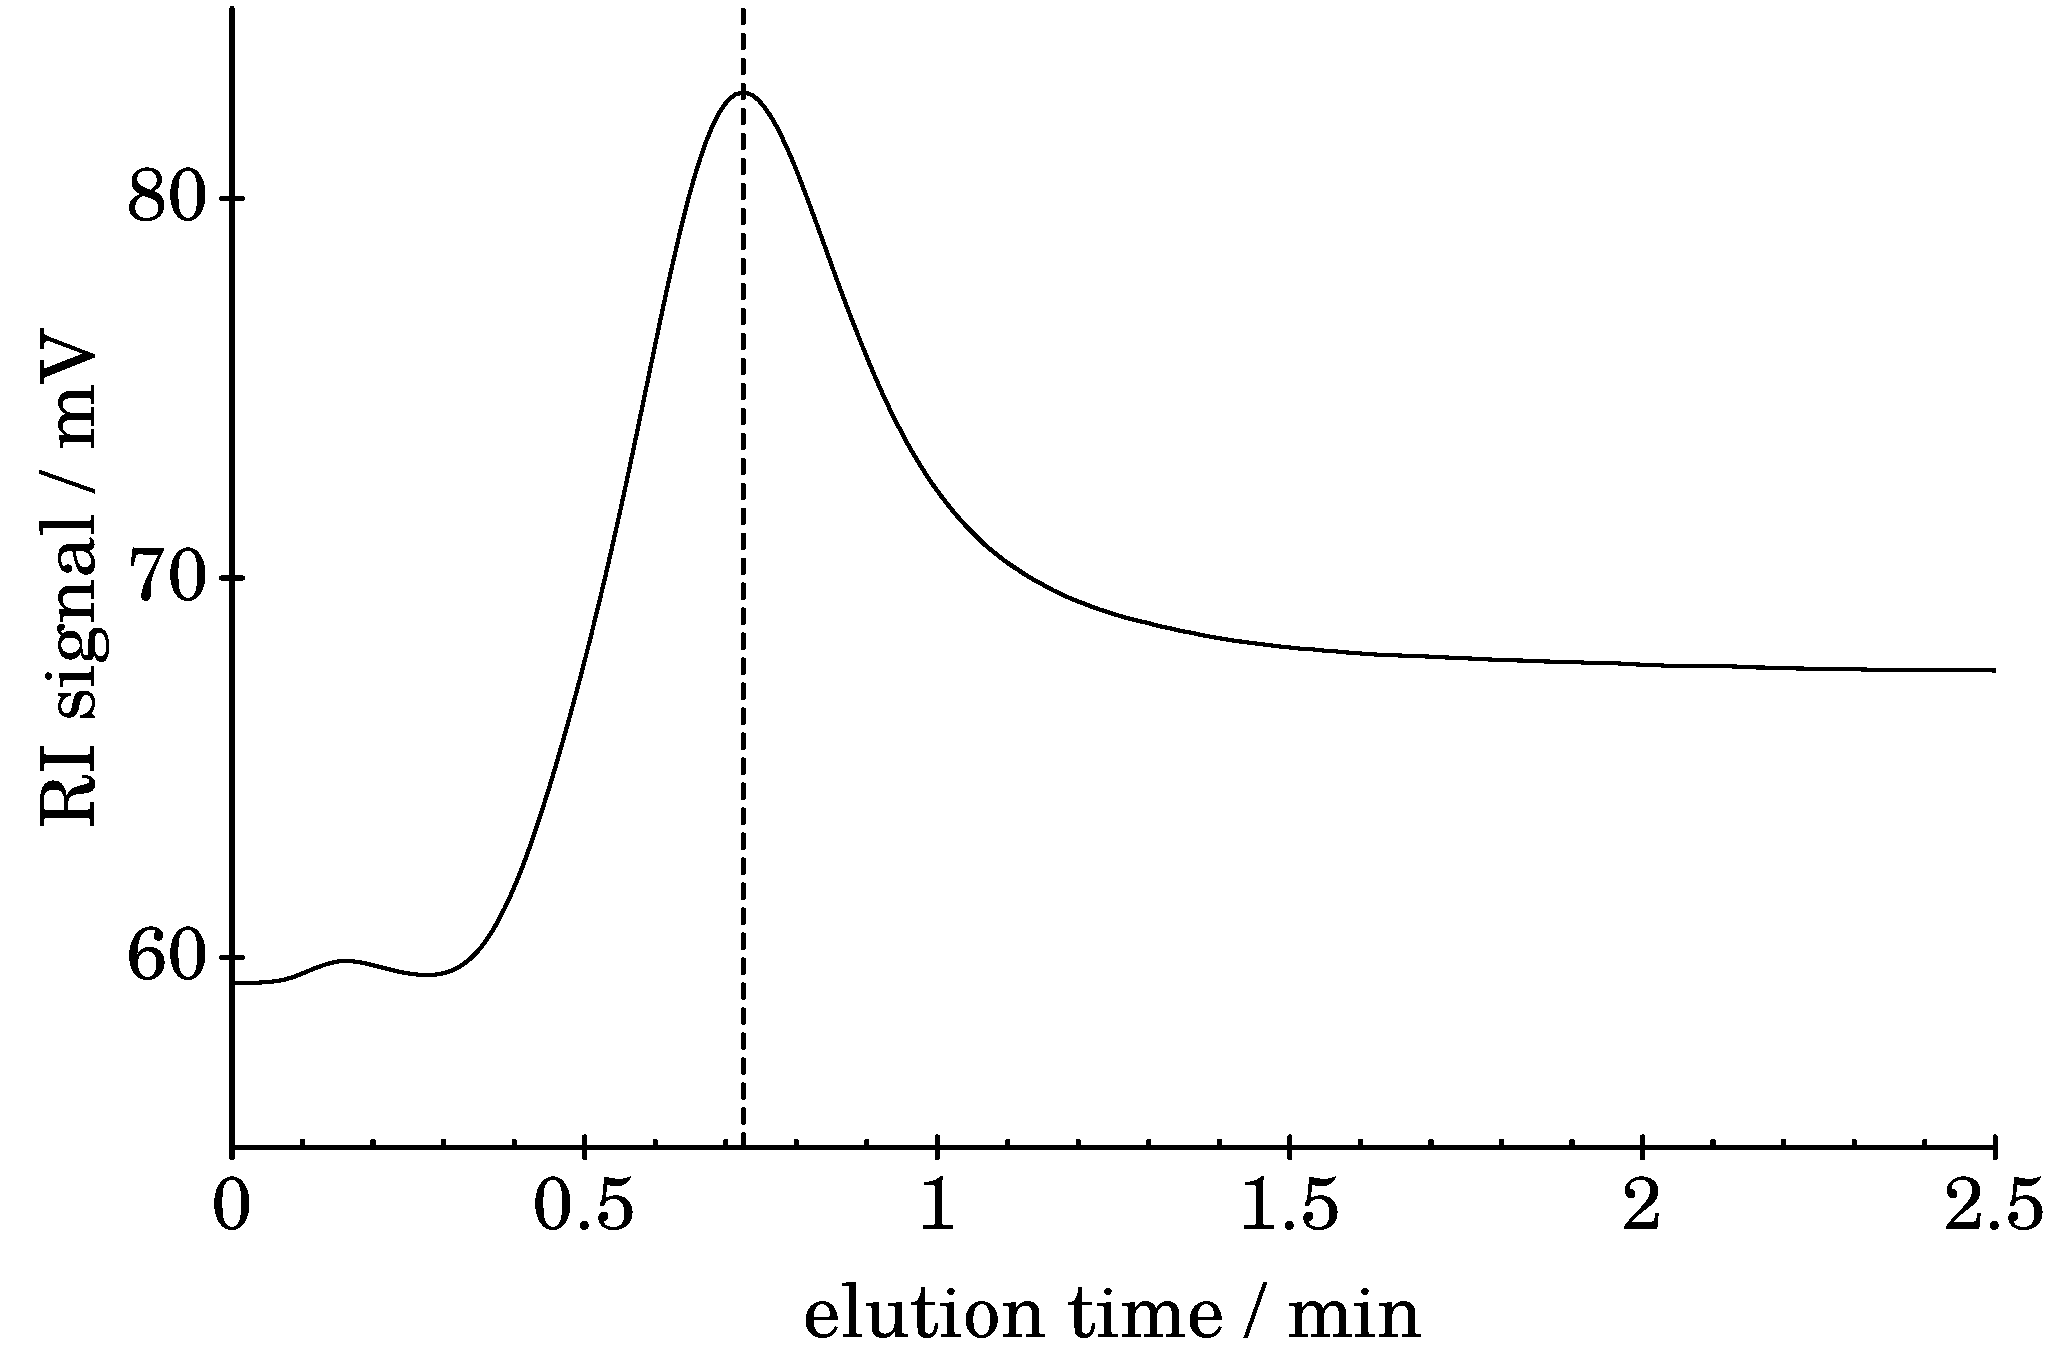
\includegraphics[width=\linewidth]{./images/data/rawPlots/img_PS_VC_05_rep1_t0_RI.pdf}
    \subcaption{Detailed starting section of fractogram \ref{subfig:raw_PS2_5_r1_te_RI}
  with RI detection signal and position of $\tvoid$.}
\end{subfigure}
  \end{center}
\vspace*{-3ex}    
\caption[Raw fractograms of PS measurements at $\Vc = \SI{0.5}{\mlmin}$, replicate 1.]{
Raw fractograms of PS 
measurements at $\Vc = \SI{0.5}{\mlmin}$, replicate 1.}
\label{fig:raw_PS_0_5_rep1} 
\end{figure}\needspace{10ex}
%%%%%%%%%%%%%%%%%%%%%%%%%%%%%%%%%%%%%%%%%%5
%%% PS at Vc = 0.5 ml/min, replicate 2
%%%%%%%%%%%%%%%%%%%%%%%%%%%%%%%%%%%%%%%%
\begin{figure}[b!]
  \begin{center}
    \begin{subfigure}{\subFigSize}
      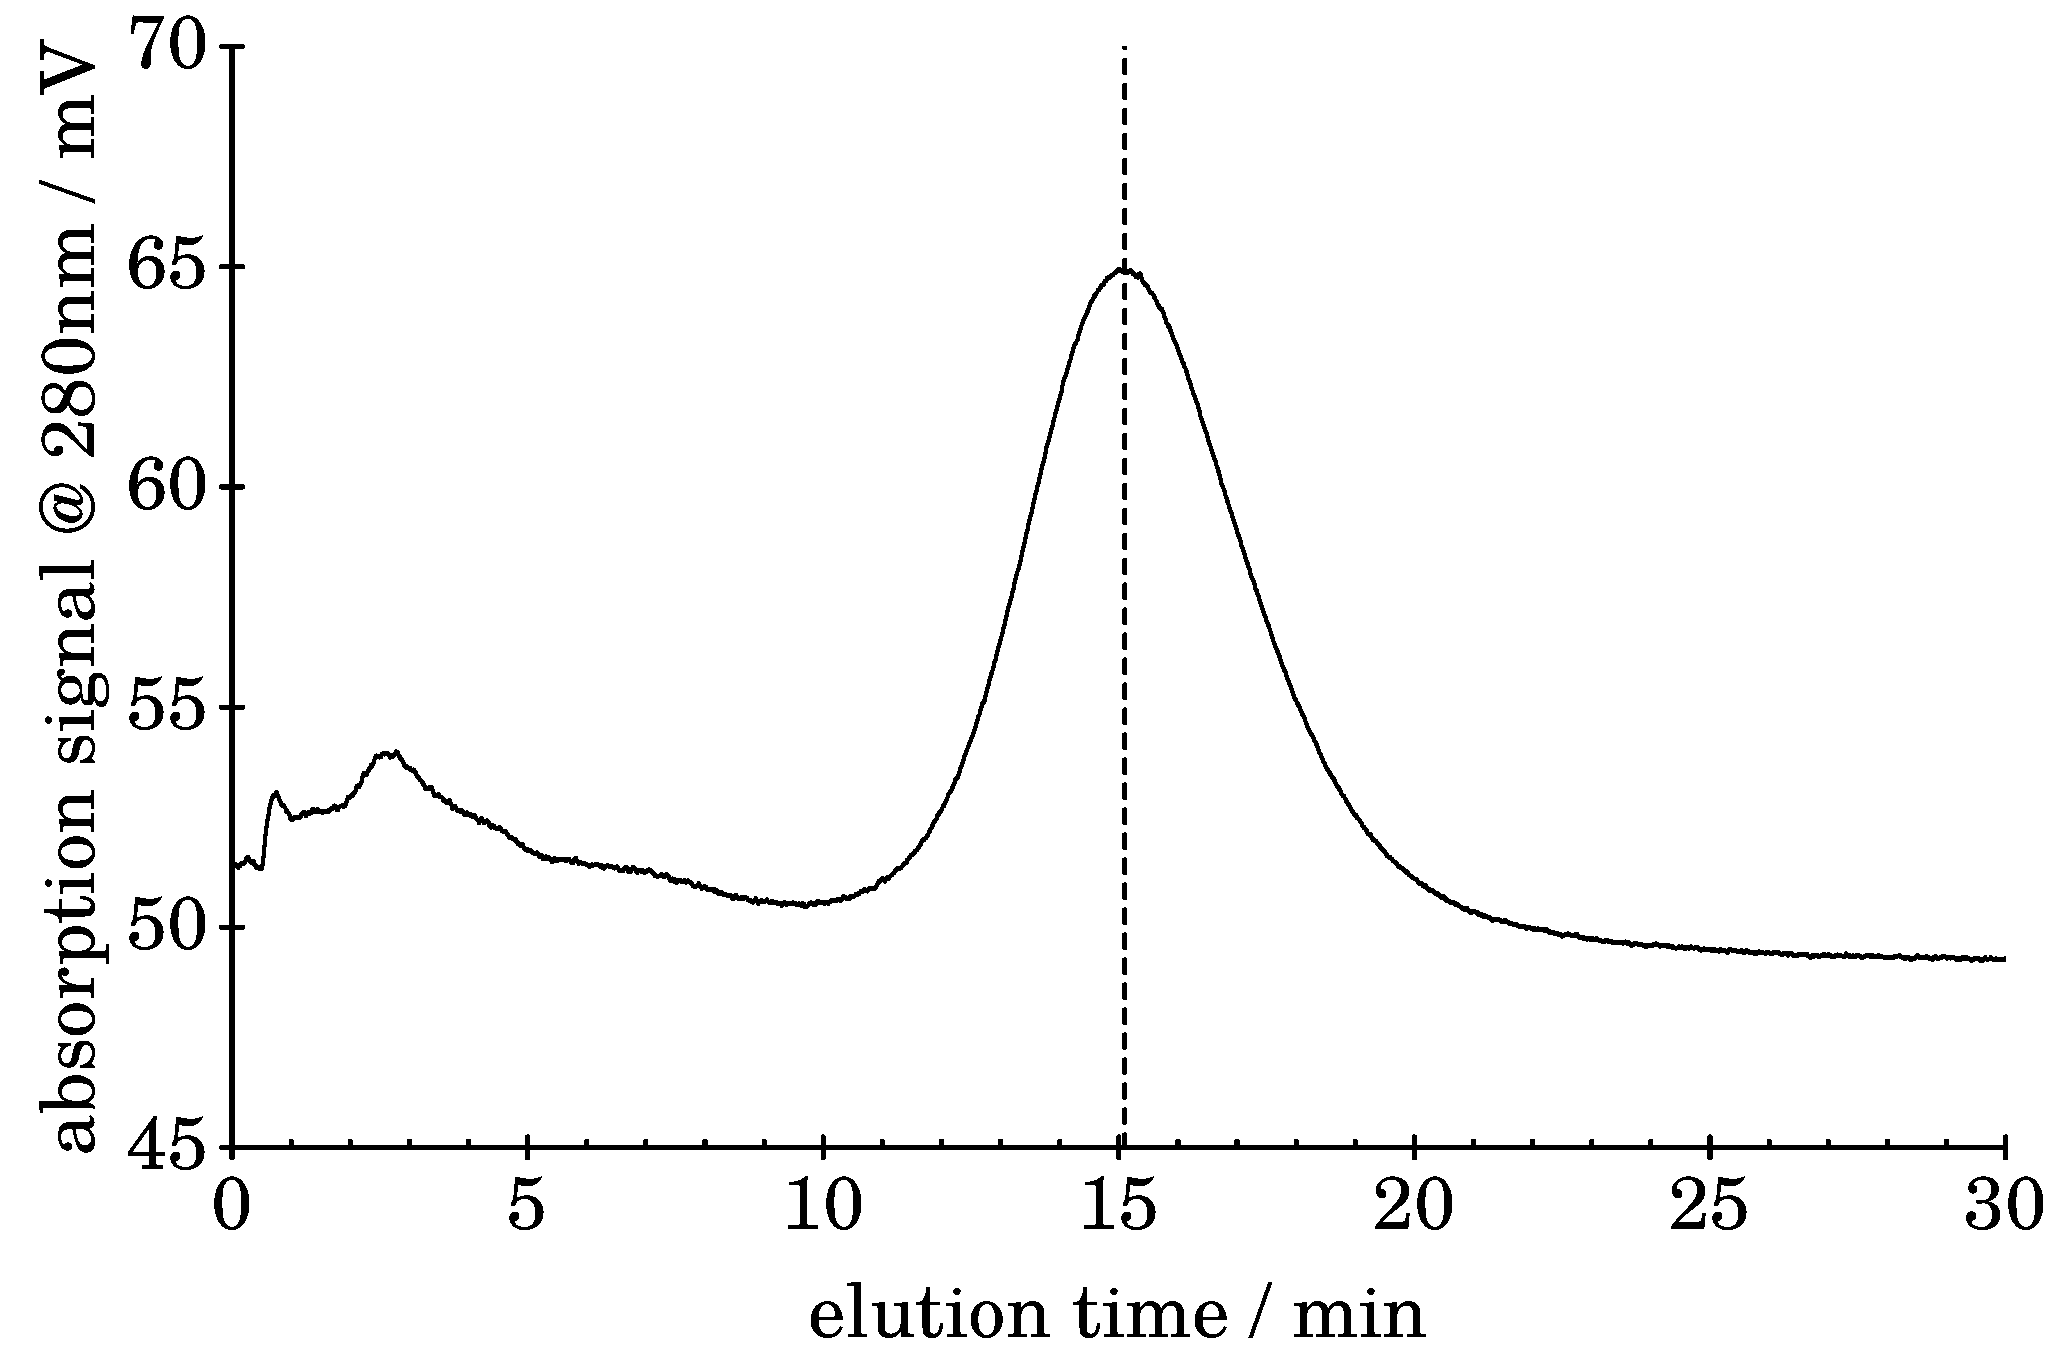
\includegraphics[width=\linewidth]{./images/data/rawPlots/img_PS_VC_05_rep2_te_UV.pdf}
      \subcaption{Position of $\te$ with UV detection signal}
      \label{subfig:raw_PS2_5_r2_te_UV}
    \end{subfigure}
    \begin{subfigure}{\subFigSize}
      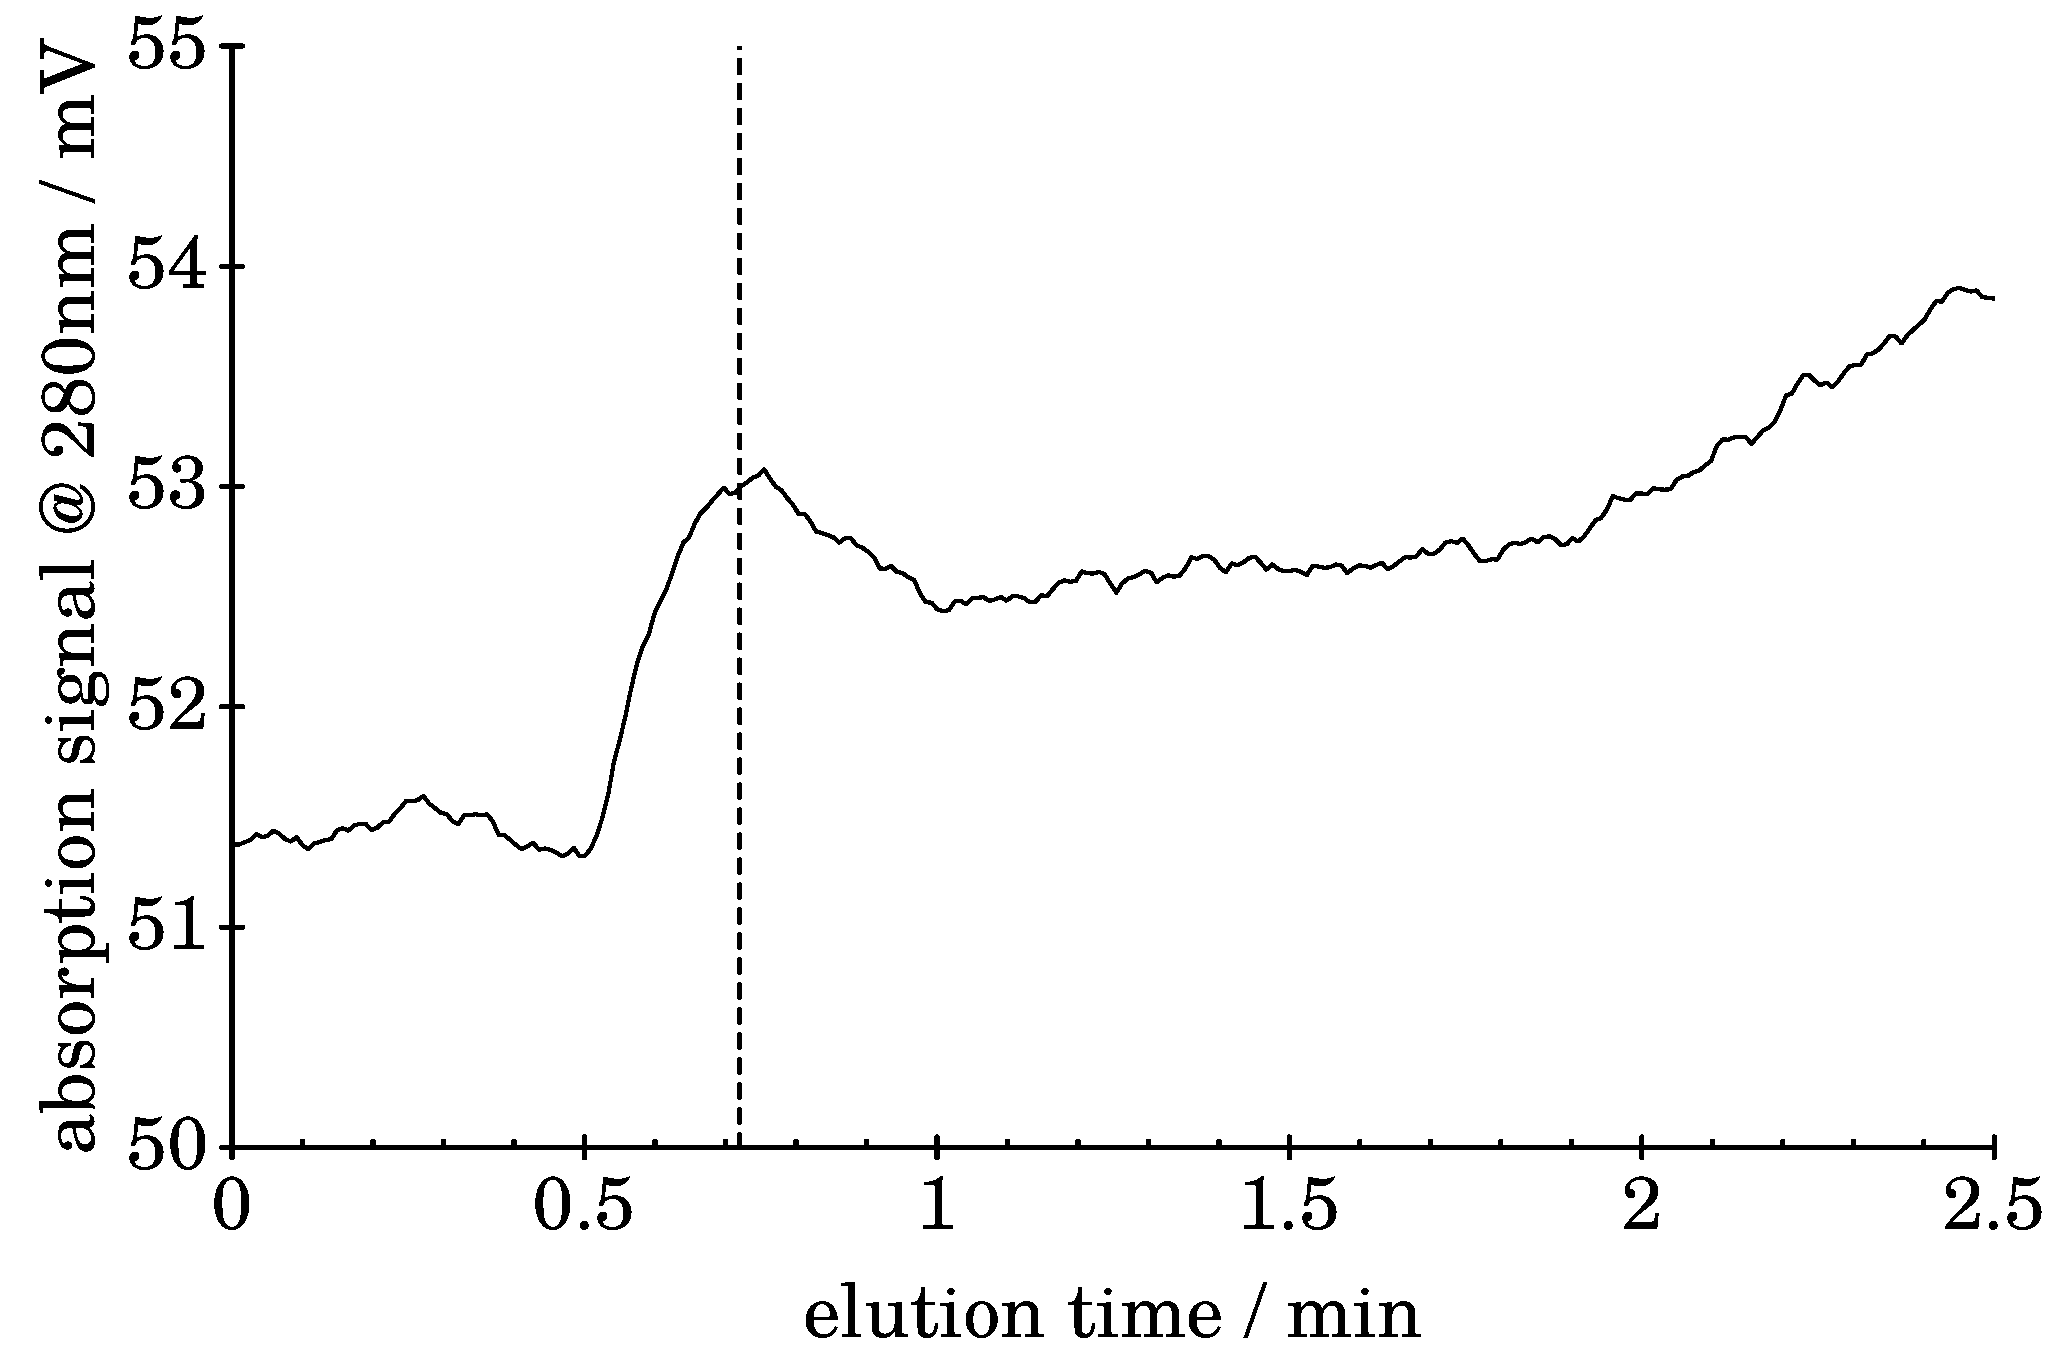
\includegraphics[width=\linewidth]{./images/data/rawPlots/img_PS_VC_05_rep2_t0_UV.pdf}
      \subcaption{Detailed starting section of fractogram \ref{subfig:raw_PS2_5_r2_te_UV}
        with UV detection signal and position of $\tvoid$.}
    \end{subfigure}
    %%%%%%%%%%%%%%%%%%
    \\\vspace*{.5em}
    %%%%%%%%%%%%%%
    \begin{subfigure}{\subFigSize} 
      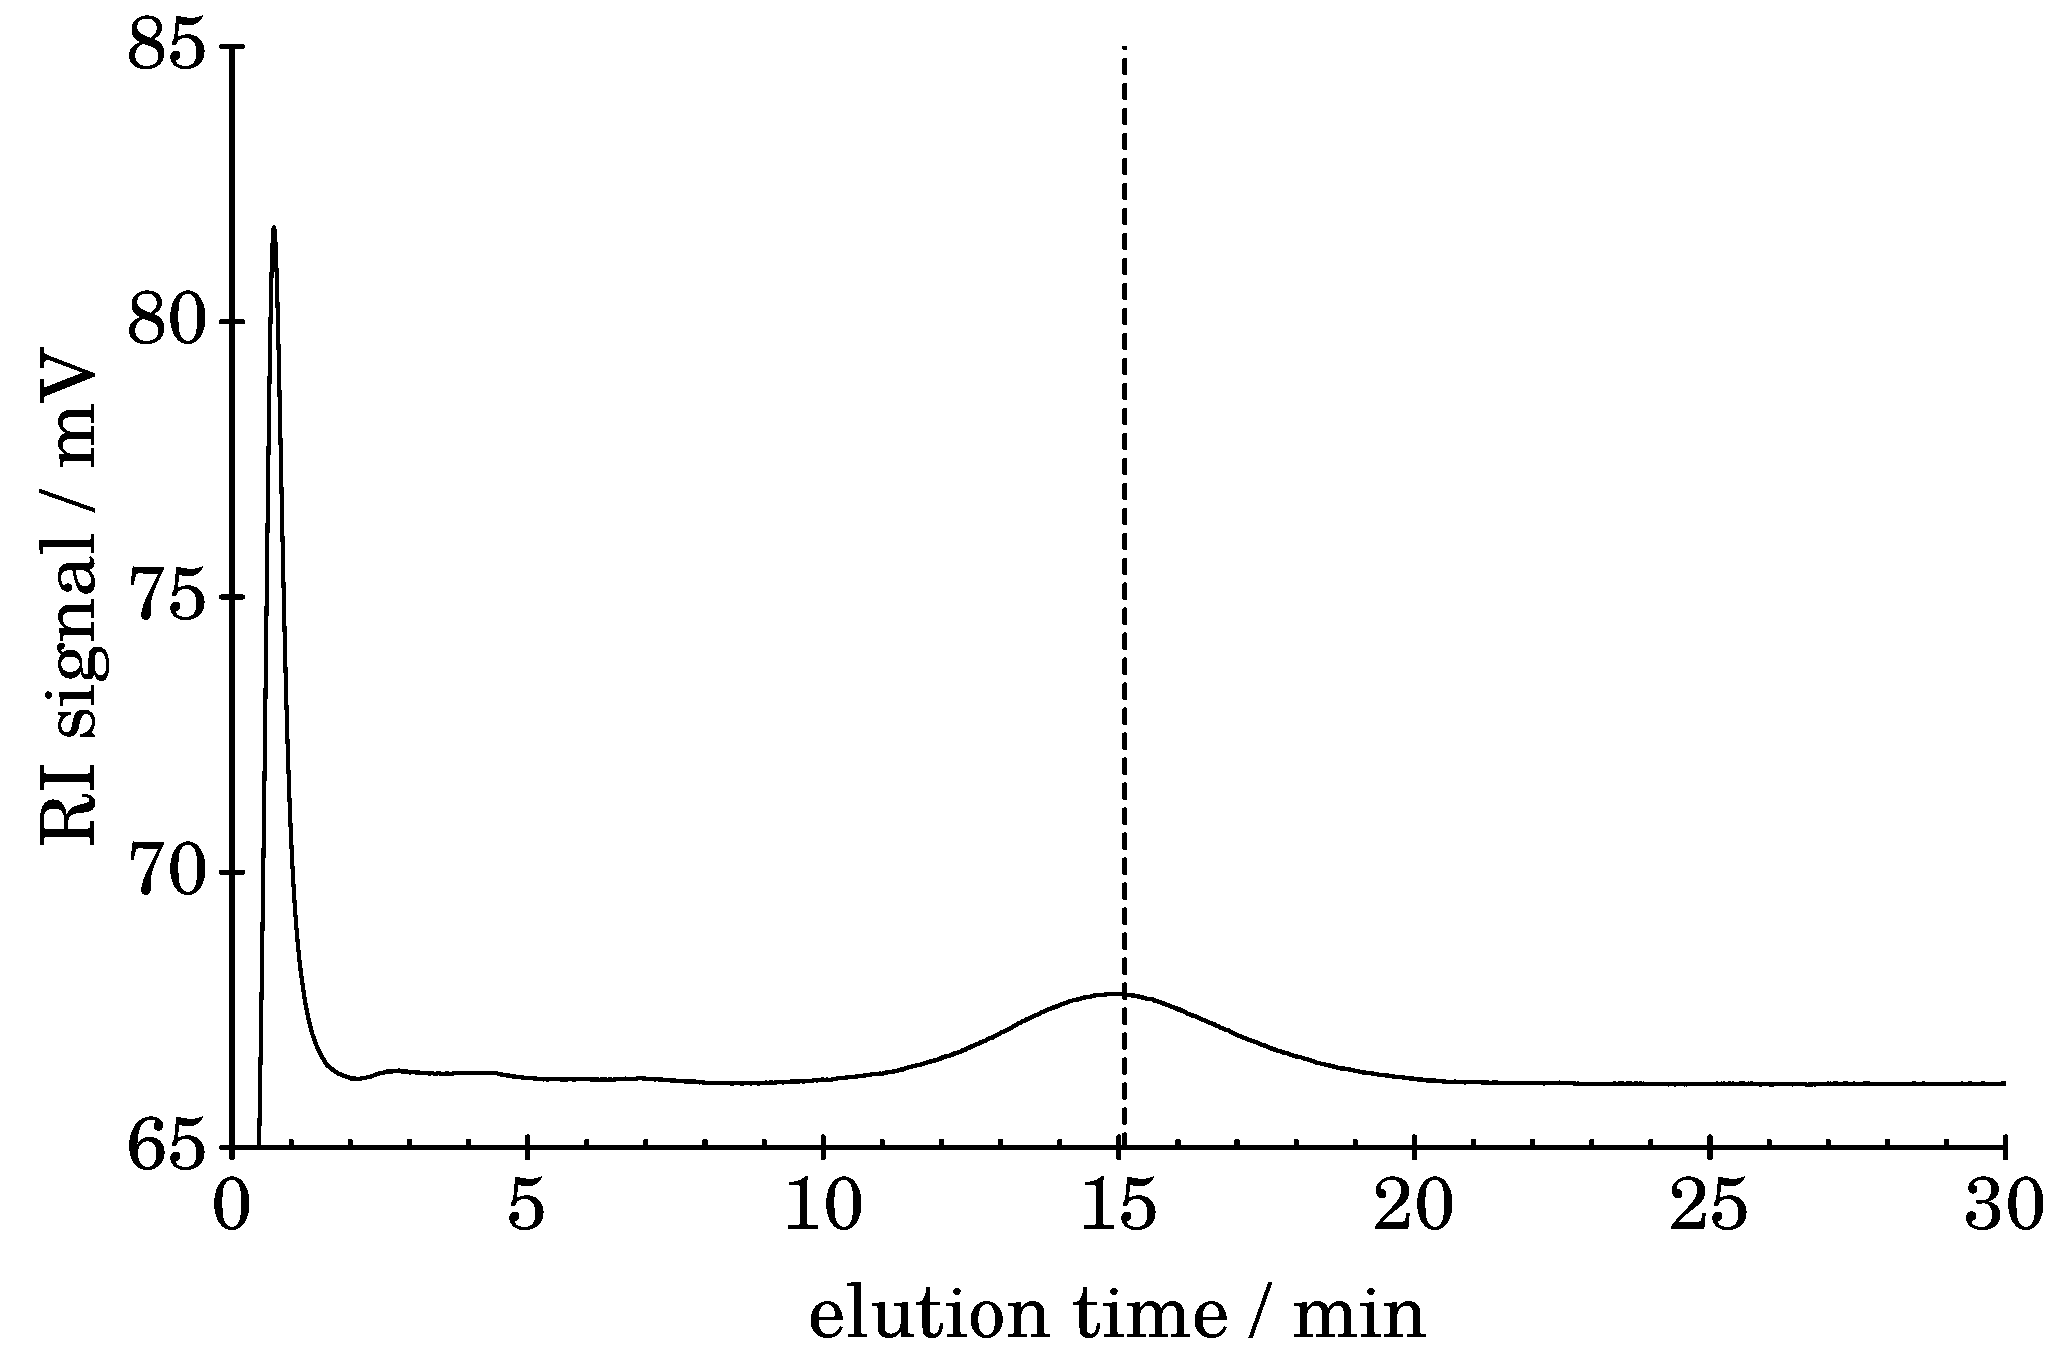
\includegraphics[width=\linewidth]{./images/data/rawPlots/img_PS_VC_05_rep2_te_RI.pdf}
      \subcaption{Position of $\te$ with RI detection signal}
      \label{subfig:raw_PS2_5_r2_te_RI}
    \end{subfigure}
    \begin{subfigure}{\subFigSize}
      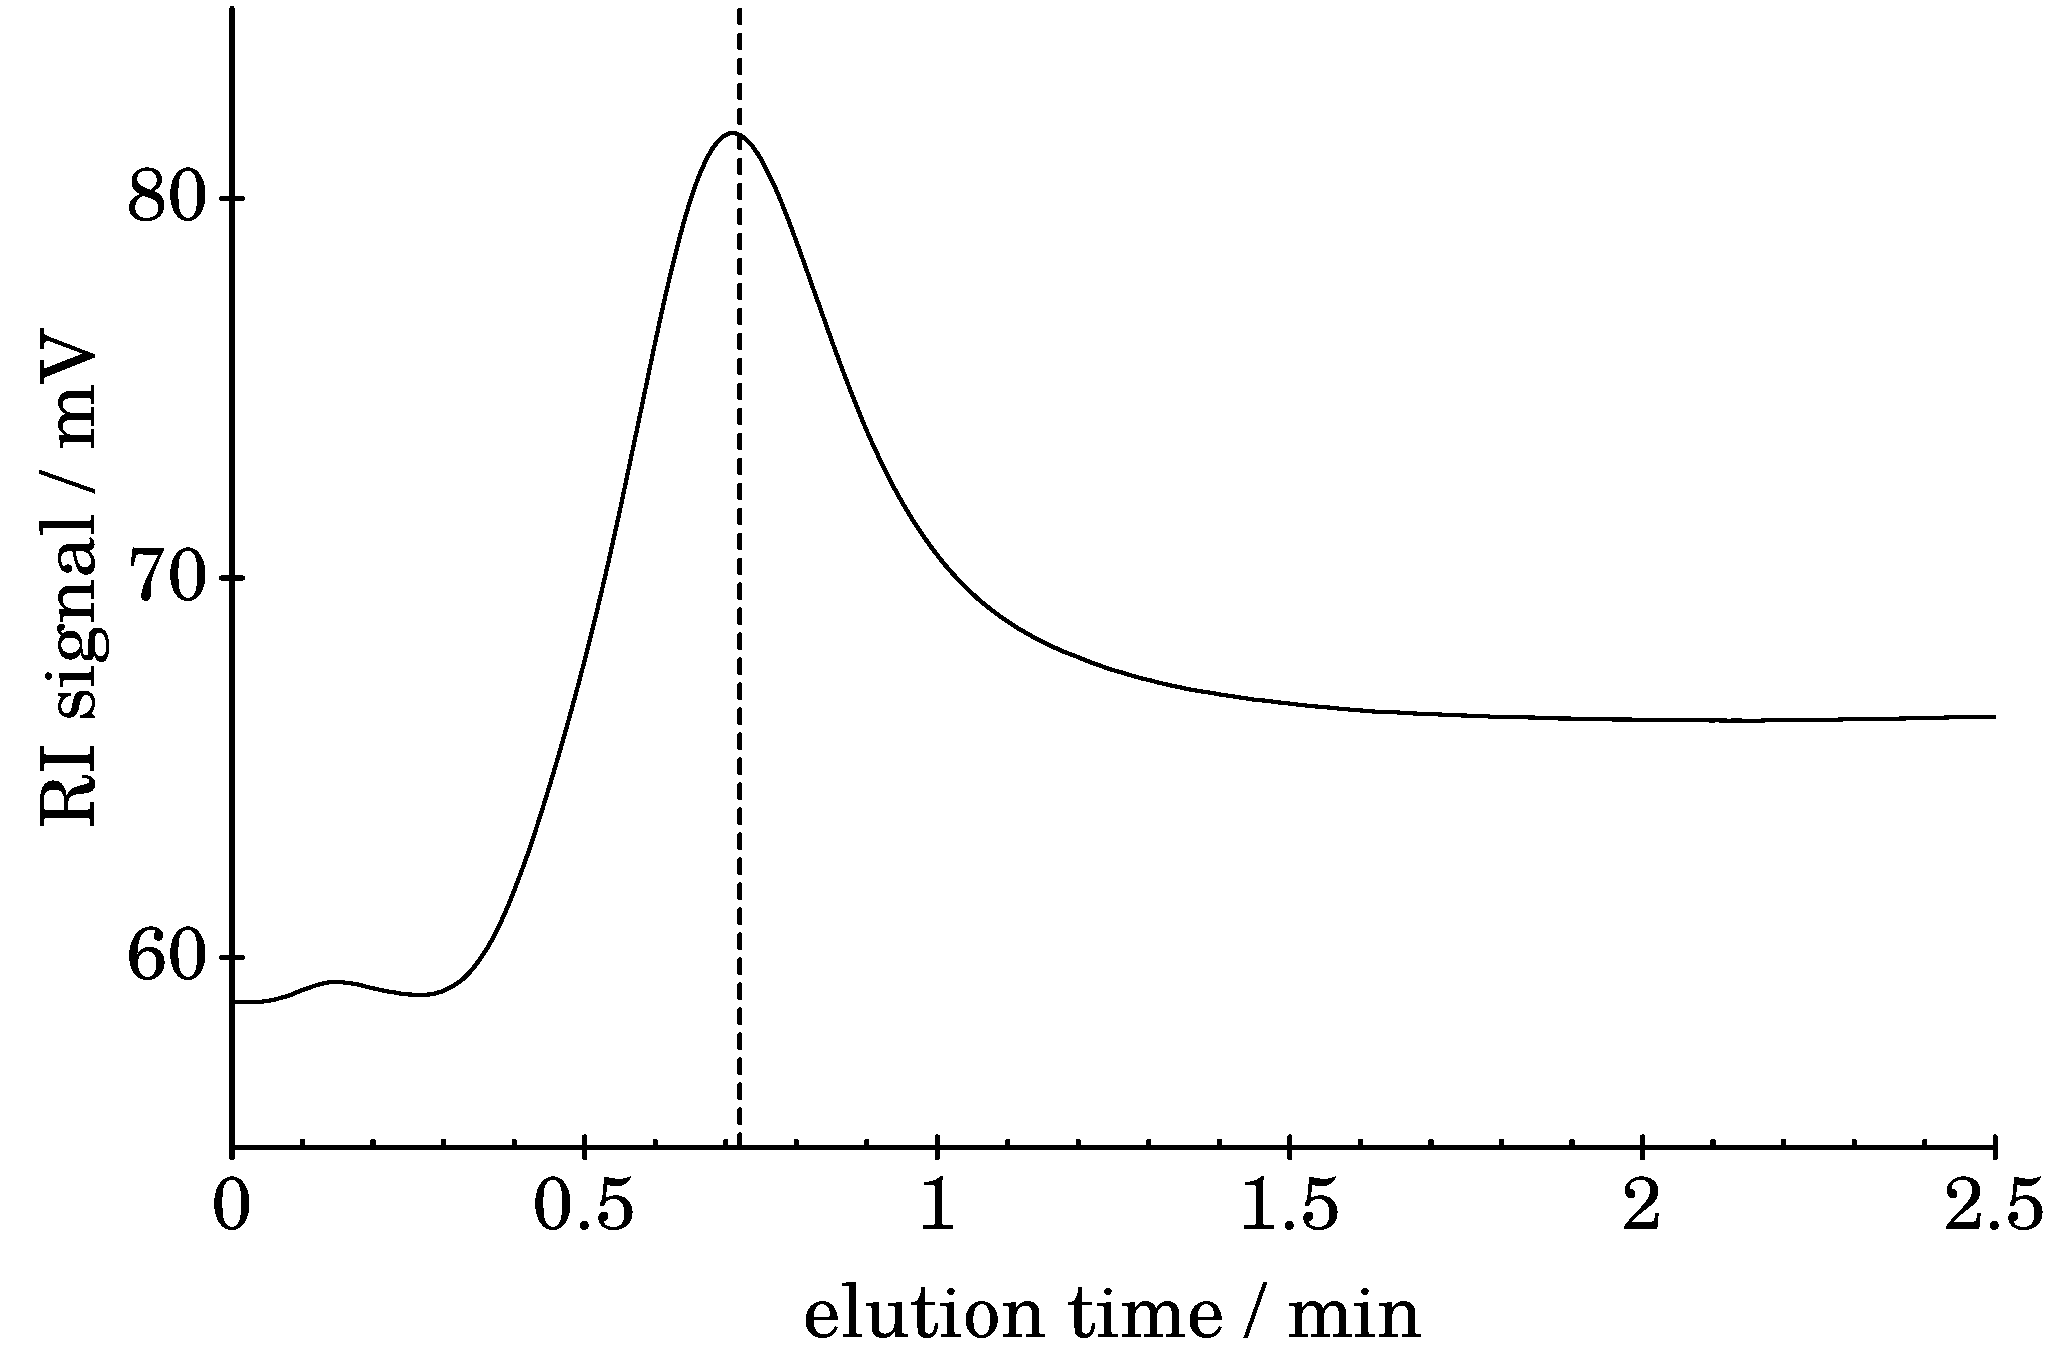
\includegraphics[width=\linewidth]{./images/data/rawPlots/img_PS_VC_05_rep2_t0_RI.pdf}
      \subcaption{Detailed starting section of fractogram \ref{subfig:raw_PS2_5_r2_te_RI}
        with RI detection signal and position of $\tvoid$.}
    \end{subfigure}
  \end{center}
  \vspace*{-3ex}    
  \caption[Raw fractograms of PS measurements at $\Vc = \SI{0.5}{\mlmin}$, replicate 2.]{
    Raw fractograms of PS 
    measurements at $\Vc = \SI{0.5}{\mlmin}$, replicate 2.}
  \label{fig:raw_PS_0_5_rep2} 
\end{figure}
%%%%%%%%%%%%%%%%%%%%%%%%%%%%%%%%%%%%%%%%%
%%% PS at Vc = 0.5 ml/min, replicate 3
%%%%%%%%%%%%%%%%%%%%%%%%%%%%%%%%%%%%%%%%
\begin{figure}[H]
  \begin{center}
    \begin{subfigure}{\subFigSize}
      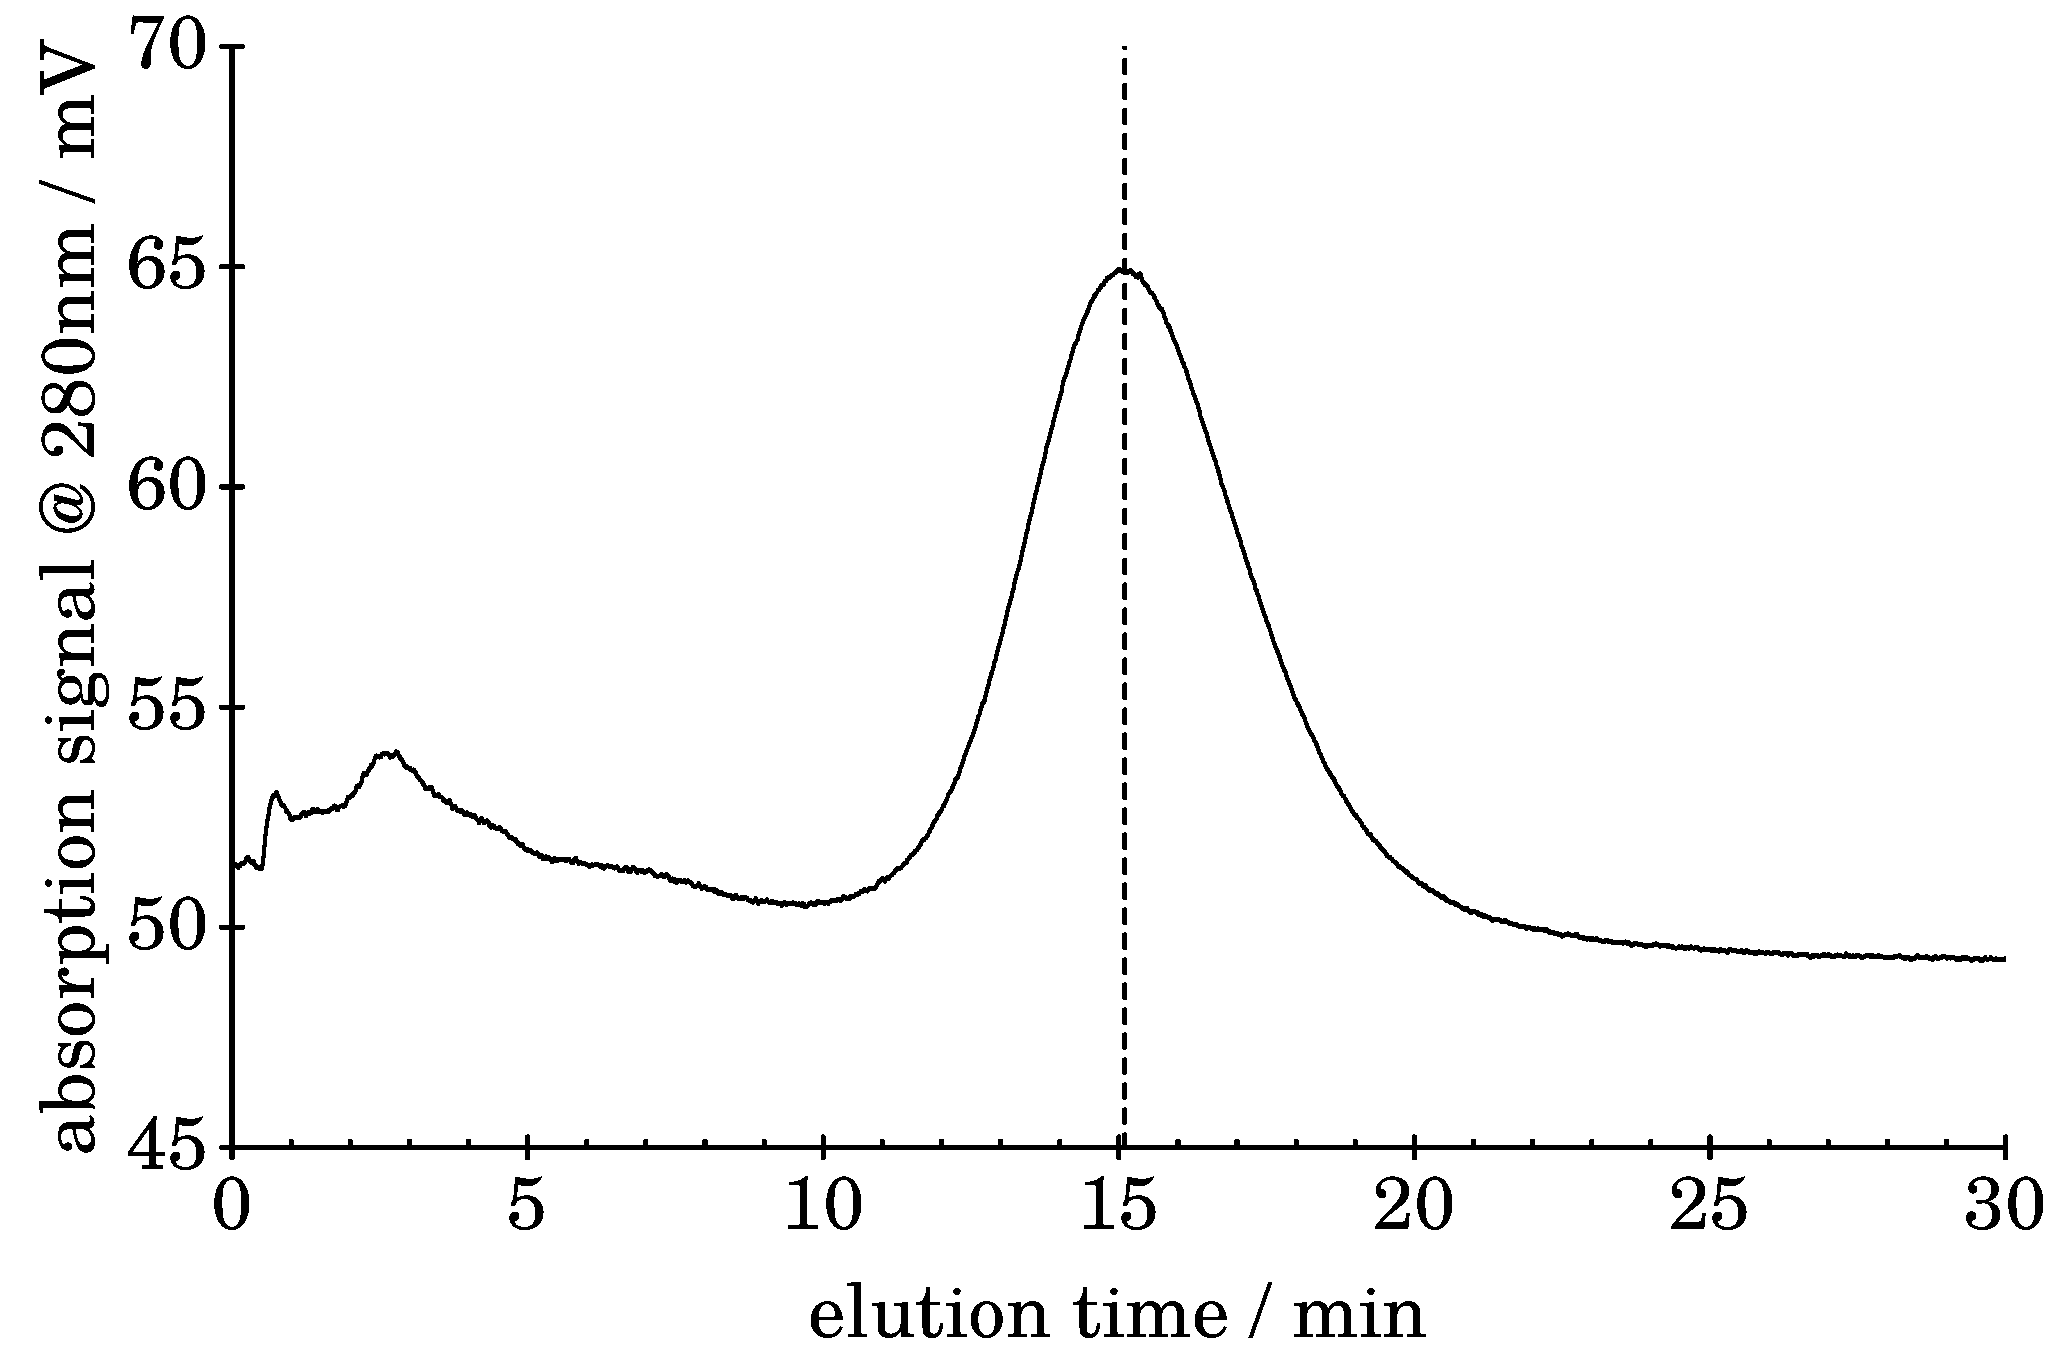
\includegraphics[width=\linewidth]{./images/data/rawPlots/img_PS_VC_05_rep2_te_UV.pdf}
      \subcaption{Position of $\te$ with UV detection signal}
      \label{subfig:raw_PS2_5_r3_te_UV}
    \end{subfigure}
    \begin{subfigure}{\subFigSize}
      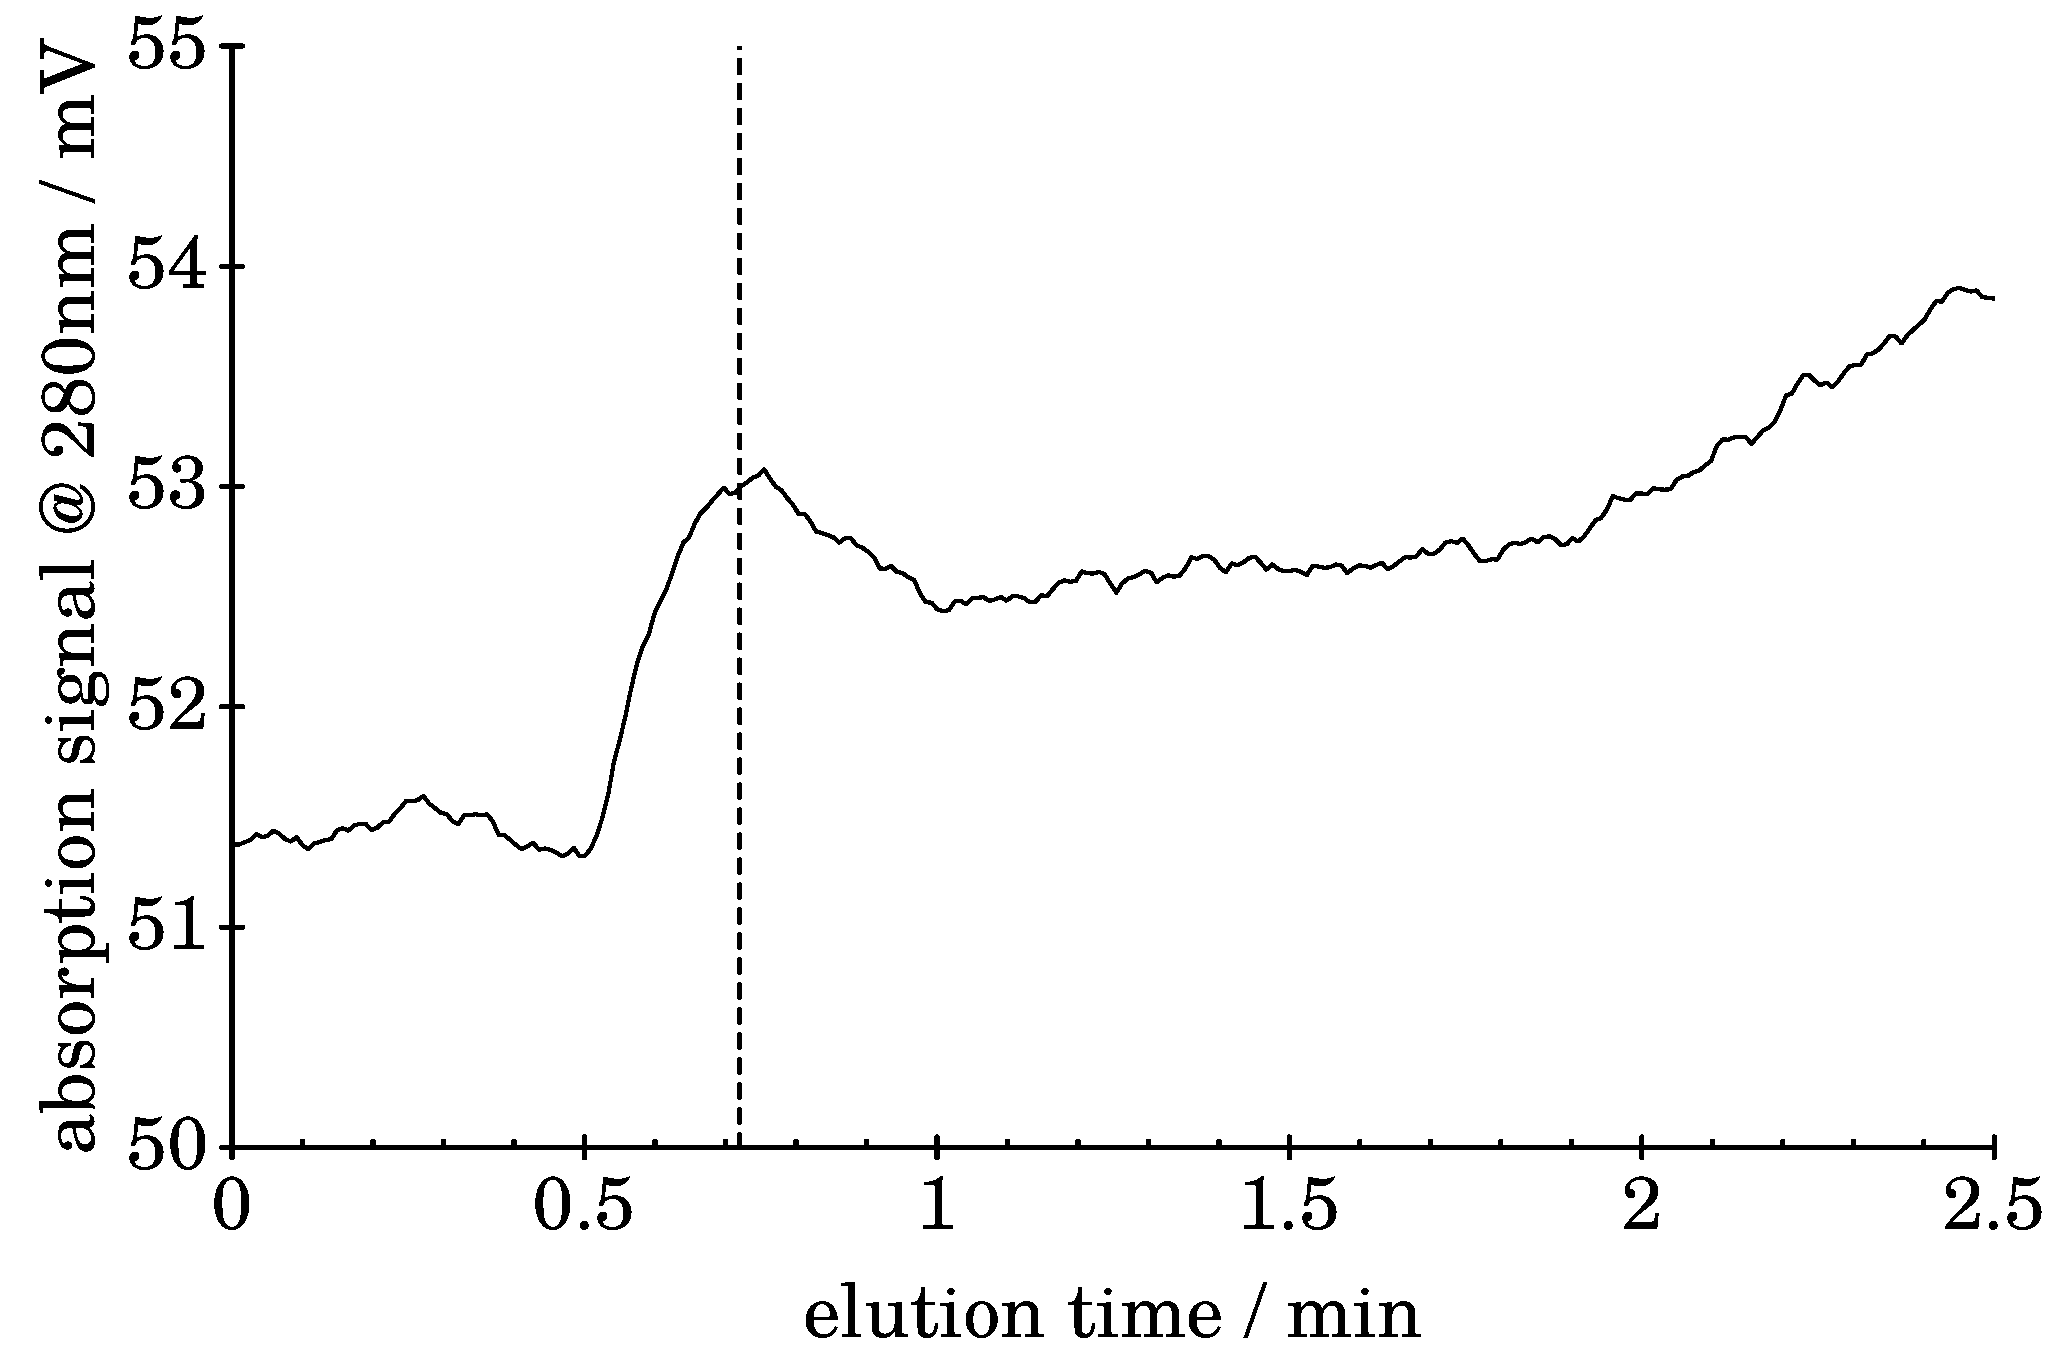
\includegraphics[width=\linewidth]{./images/data/rawPlots/img_PS_VC_05_rep2_t0_UV.pdf}
      \subcaption{Detailed starting section of fractogram \ref{subfig:raw_PS2_5_r3_te_UV}
        with UV detection signal and position of $\tvoid$.}
    \end{subfigure}
    %%%%%%%%%%%%%%%%%%
    \\\vspace*{.5em}
    %%%%%%%%%%%%%%
    \begin{subfigure}{\subFigSize} 
      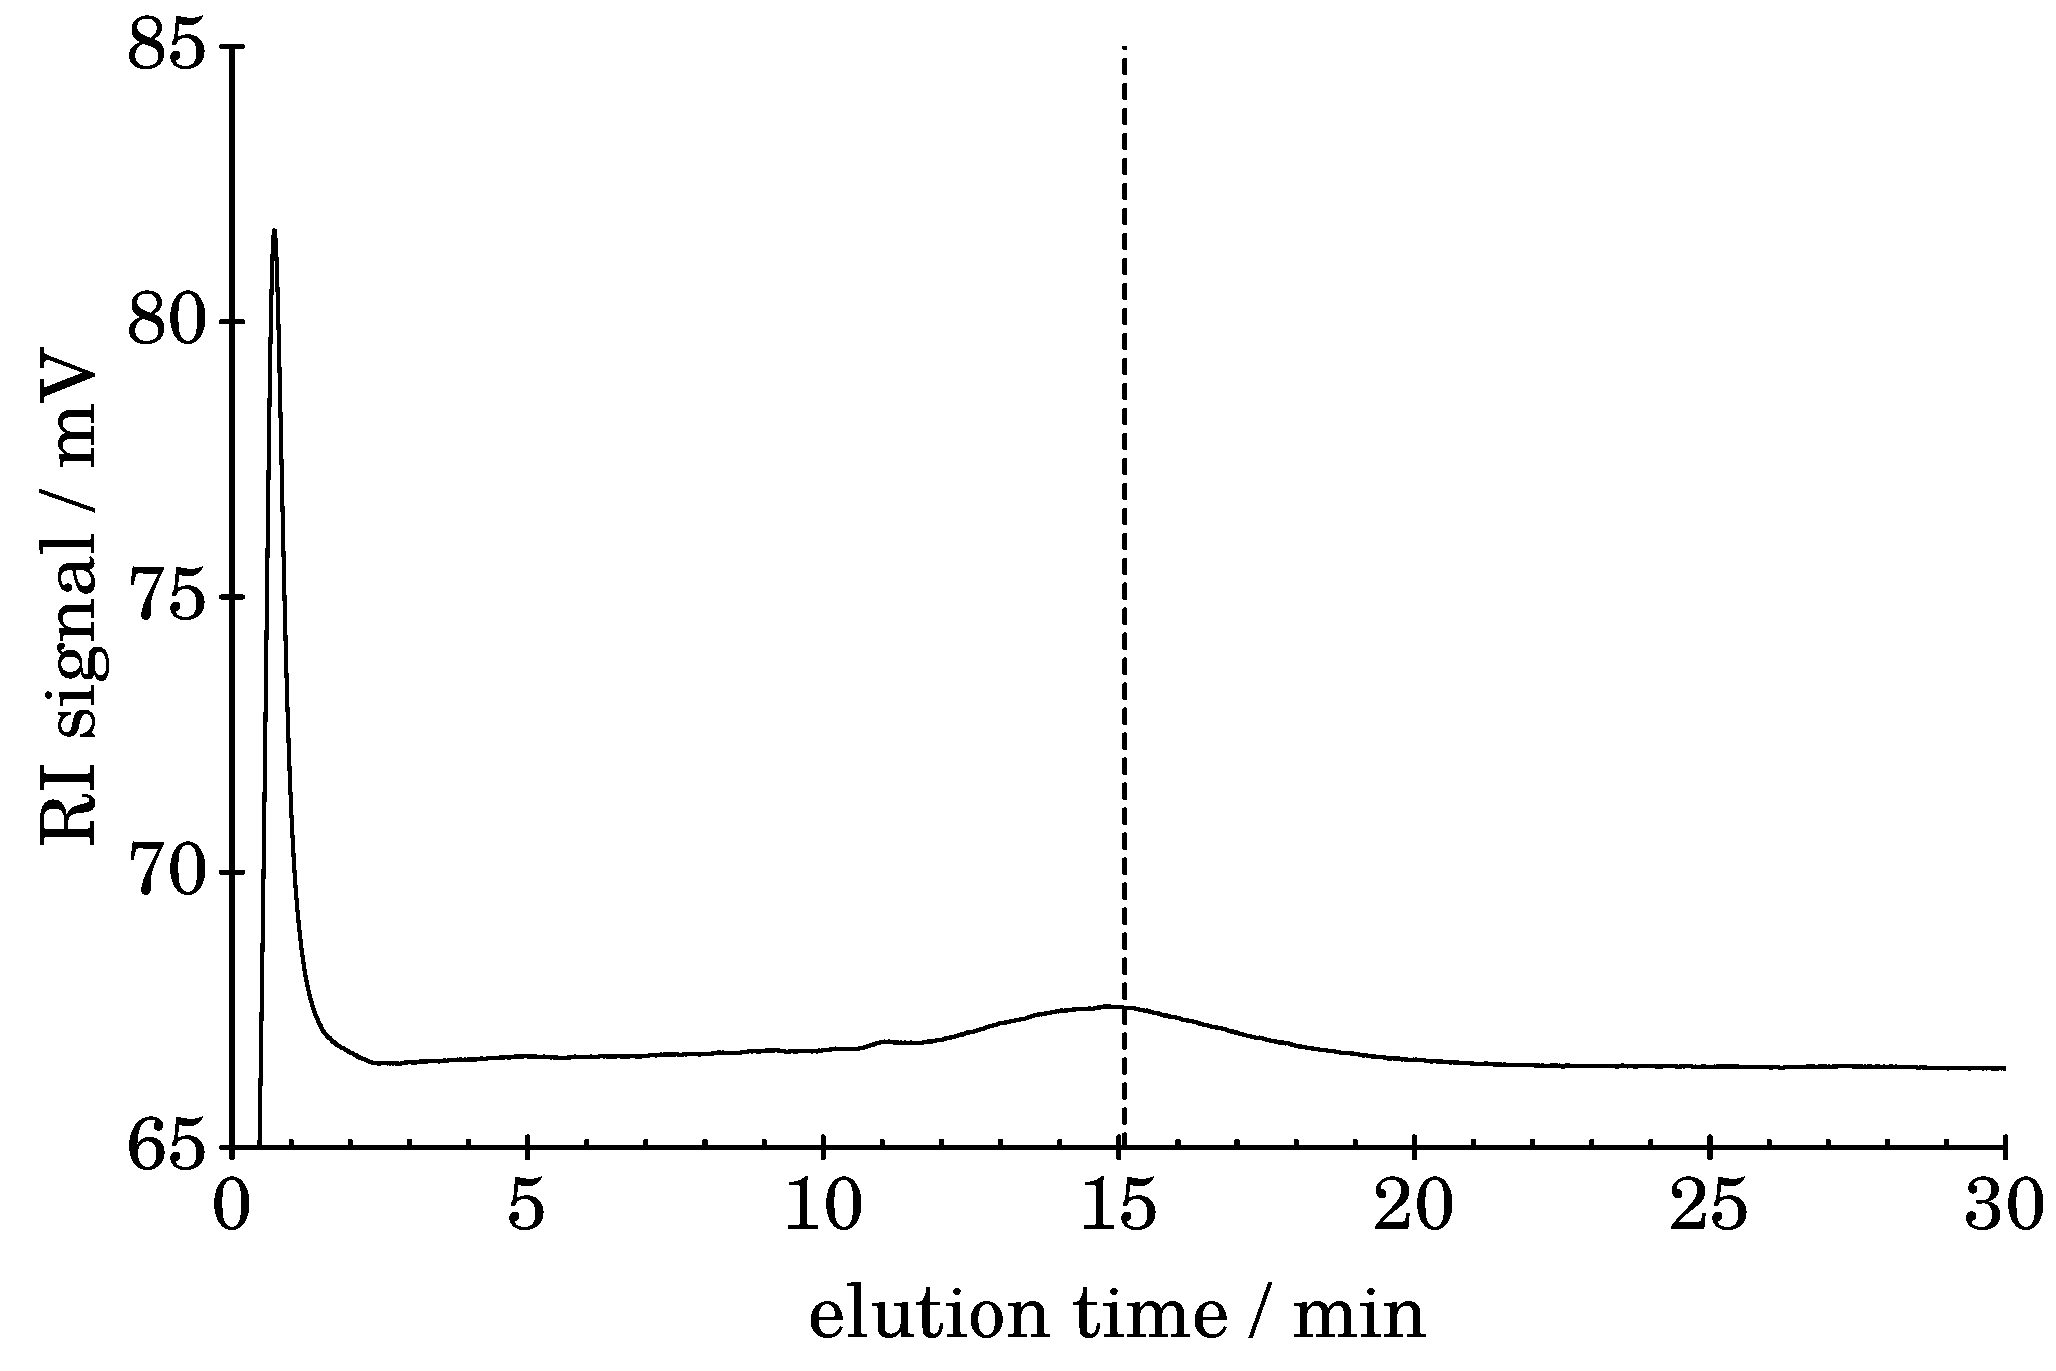
\includegraphics[width=\linewidth]{./images/data/rawPlots/img_PS_VC_05_rep3_te_RI.pdf}
      \subcaption{Position of $\te$ with RI detection signal}
      \label{subfig:raw_PS2_5_r3_te_RI}
    \end{subfigure}
    \begin{subfigure}{\subFigSize}
      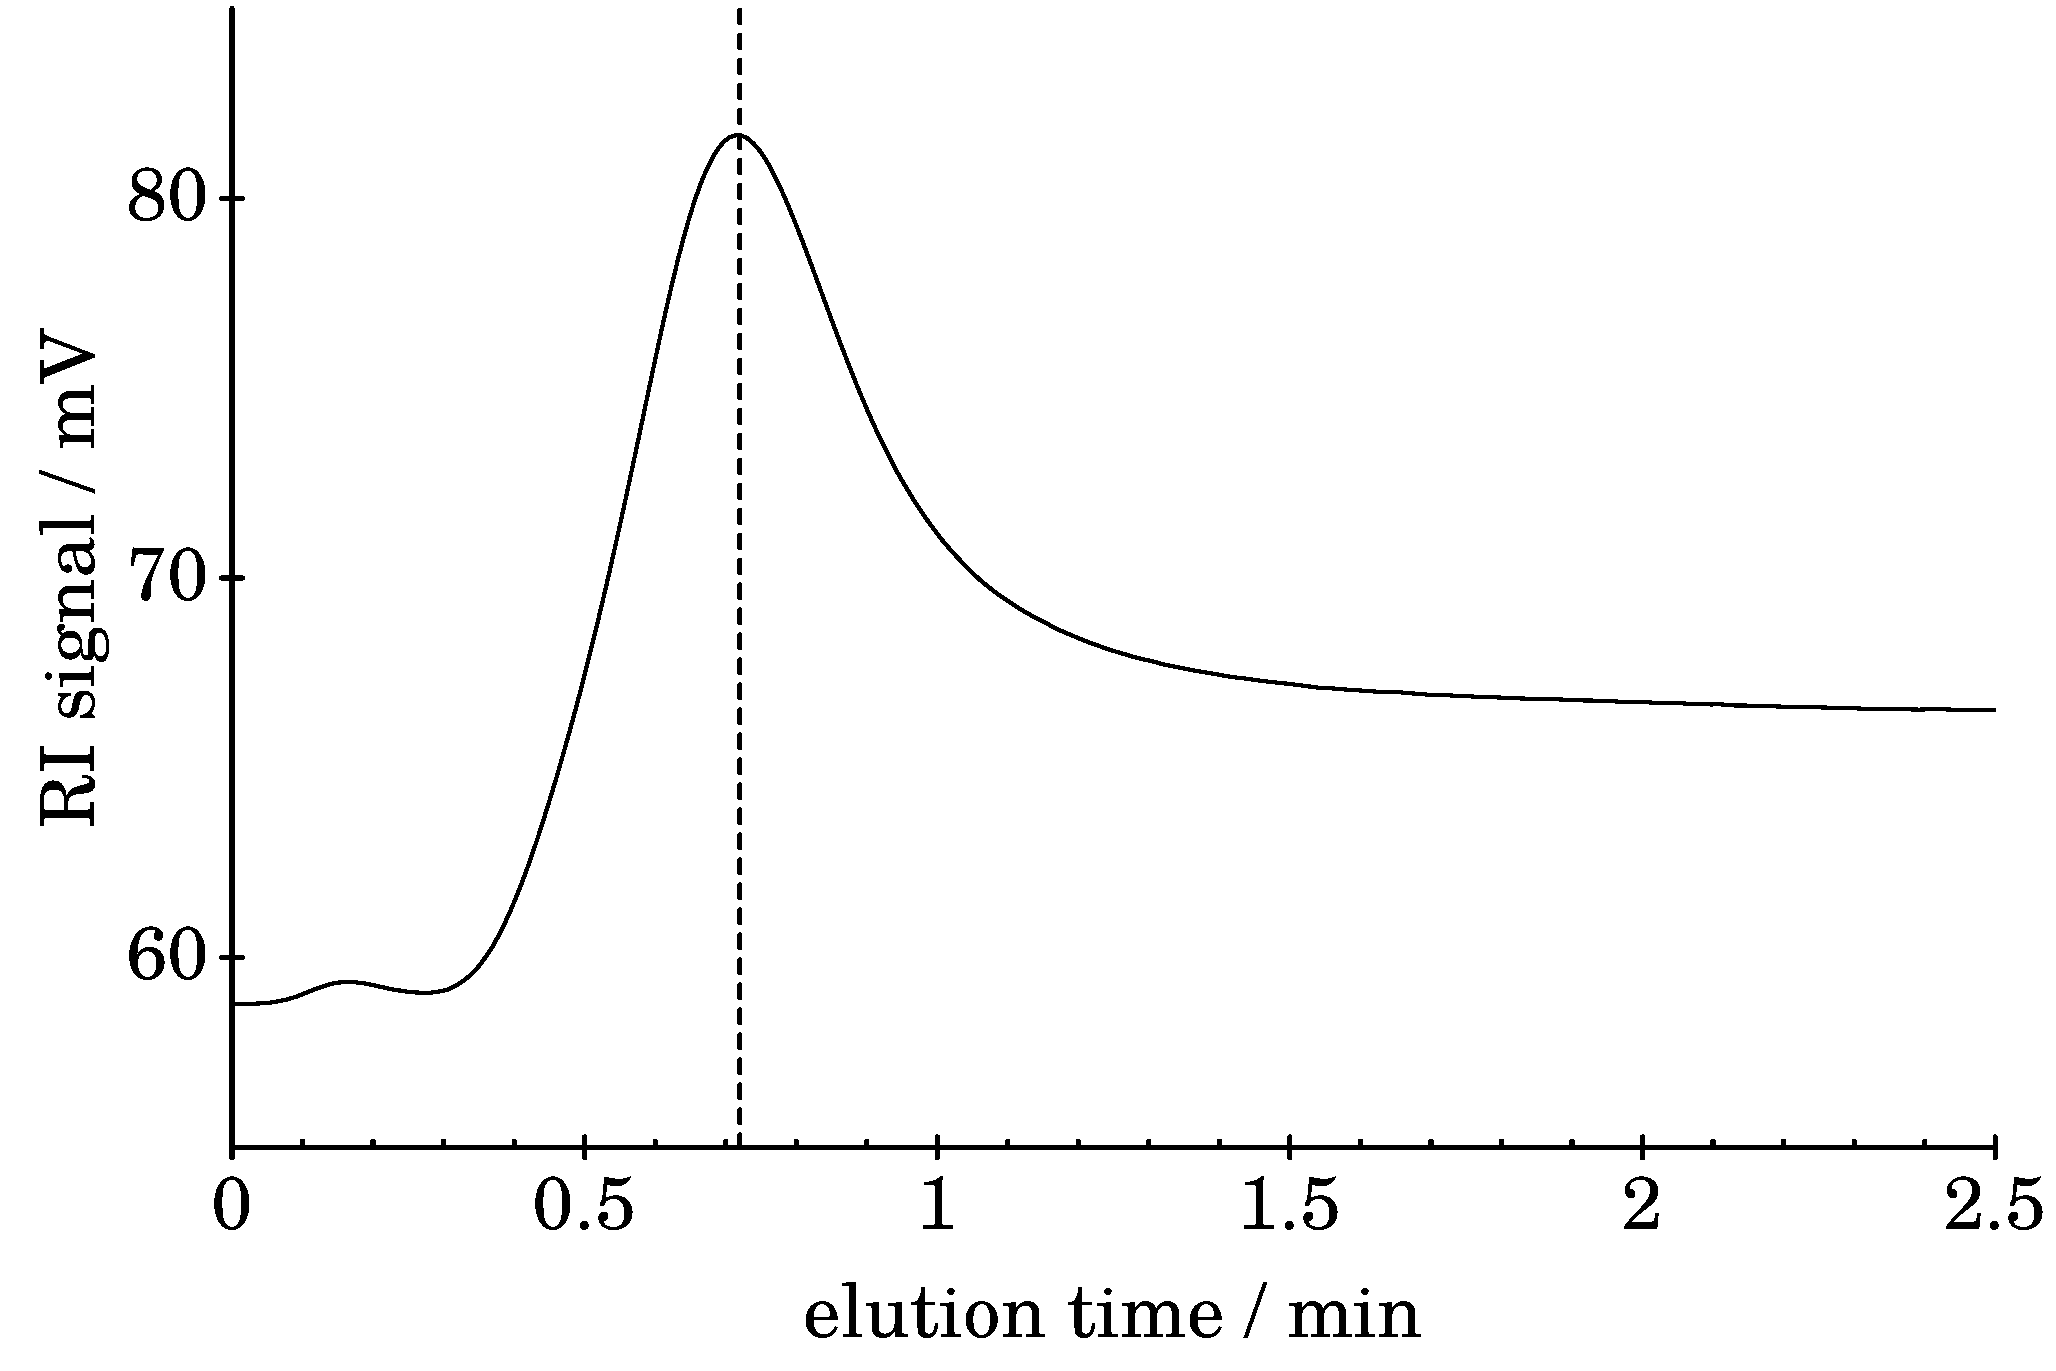
\includegraphics[width=\linewidth]{./images/data/rawPlots/img_PS_VC_05_rep3_t0_RI.pdf}
      \subcaption{Detailed starting section of fractogram \ref{subfig:raw_PS2_5_r3_te_RI}
        with RI detection signal and position of $\tvoid$.}
    \end{subfigure}
  \end{center}
  \vspace*{-3ex}    
  \caption[Raw fractograms of PS measurements at $\Vc = \SI{0.5}{\mlmin}$, replicate 3.]{
    Raw fractograms of PS 
    measurements at $\Vc = \SI{0.5}{\mlmin}$, replicate 3.}
  \label{fig:raw_PS_0_5_rep3}
\end{figure}
%\newgeometry{bottom=0.5cm}
%\newgeometry{foot=0.5cm}
\clearpage
%%%%%%%%%%%%%%%%%%%%%%%%%%%%%%%%%%%%%%%%%%%%%%%%%%%%%%%%%
%%% 
%%% Evaluated own result statistics at different z%
%%%
%%%%%%%%%%%%%%%%%%%%%%%%%%%%%%%%%%%%%%%%%%%%%%%%%%%%%%%%%
\section*{Evaluated of own calibration experiments with BSA and PS for different $\bm{\zP}$}
\renewcommand{\subFigSize}{0.49\linewidth}
%\begin{landscape}
%\thispagestyle{empty}
%%%%%%%%%%%%%%%%%%%%%%%%%%%%%%
%%% z% = 8
%%%%%%%%%%%%%%%%%%%%%%%%%%%%%
%\begin{minipage}[t]{1.1\linewidth}
\begin{figure}[htp]
  \begin{center}
    \begin{subfigure}{\subFigSize}
      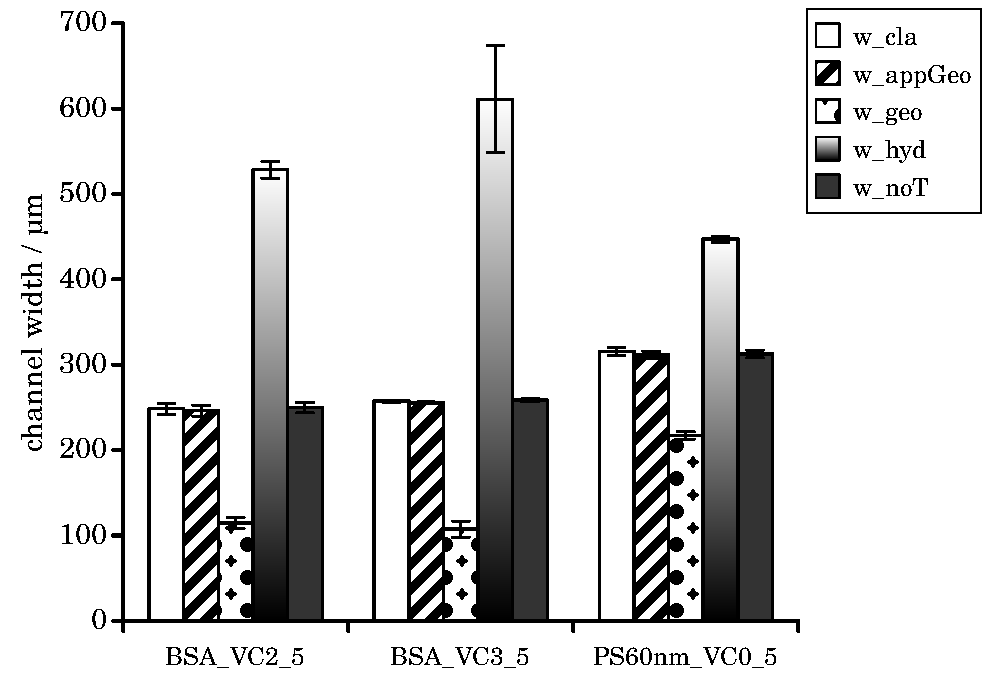
\includegraphics[width=\linewidth]{./images/data/eval_own_p8/ownData_w_p8.pdf}
      \subcaption{Calibration results for $w$}
%      \label{subfig:calibRes_BSA_VC2_5_w}
    \end{subfigure}
    \begin{subfigure}{\subFigSize}
      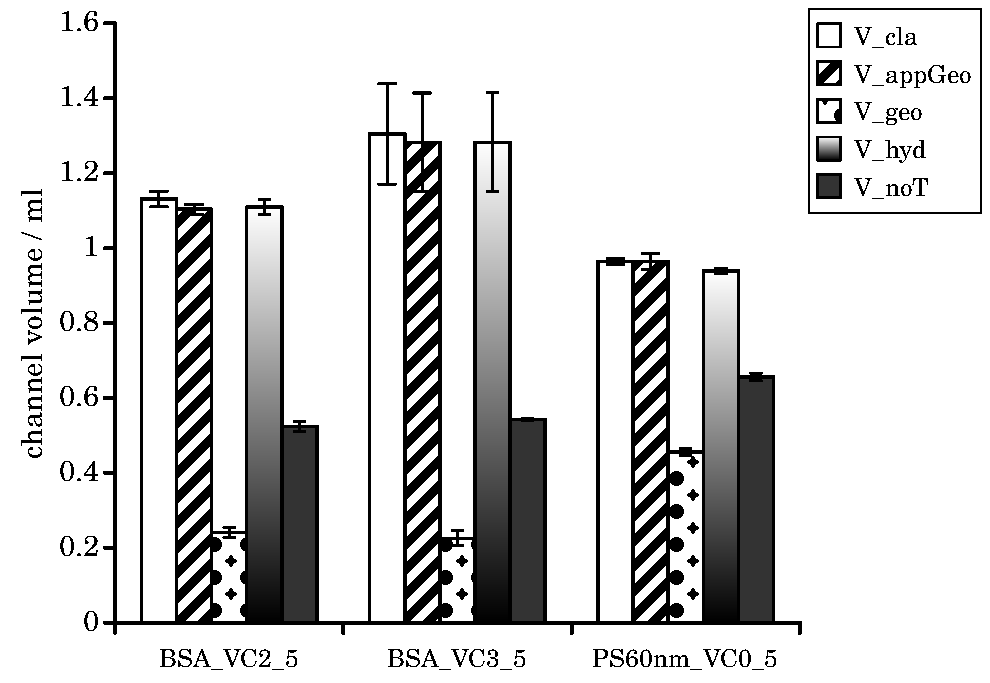
\includegraphics[width=\linewidth]{./images/data/eval_own_p8/ownData_V_p8.pdf}
      \subcaption{Calibration results for $V$}
    \end{subfigure}
  \end{center}
  \vspace*{-4ex}    
  \caption[Statistical results of $w$ and $V$ from all 5 calibration algorithms for assumed $\zP = \SI{8}{\percent}$]{
    Statistical results of $w$ and $V$ from all 5 calibration algorithms for assumed $\zP = \SI{8}{\percent}$
  }
  \label{fig:statCalibResP8}
\end{figure}  
%%%%%%%%%%%%%%%%%%%%%%%%%%%%%%
%%% z% = 12
%%%%%%%%%%%%%%%%%%%%%%%%%%%%%
\begin{figure}[htp]
  \begin{center}
    \begin{subfigure}{\subFigSize}
      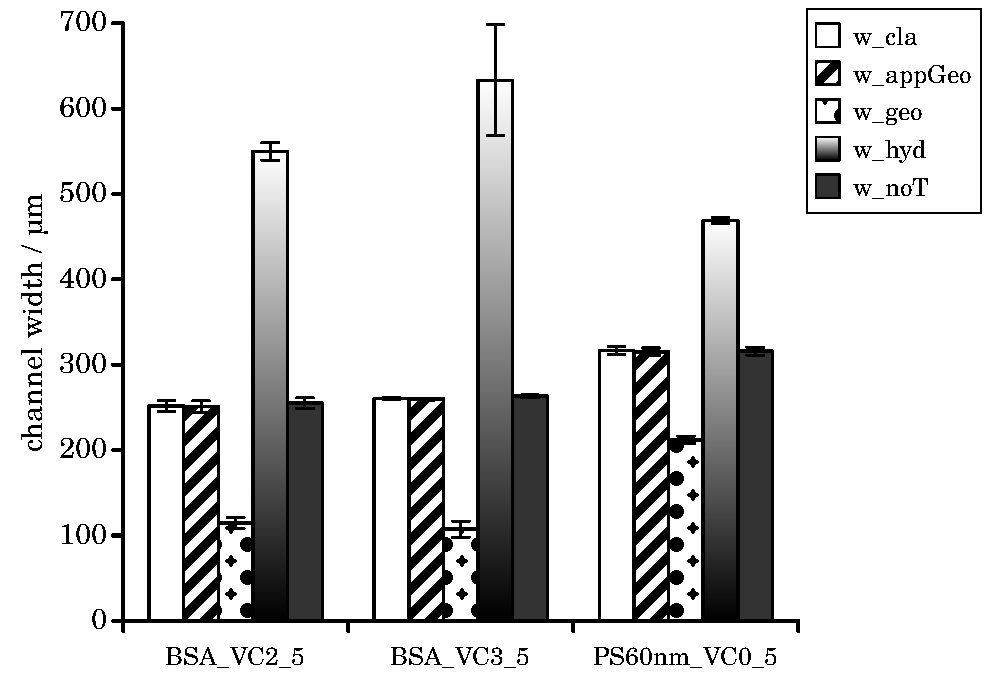
\includegraphics[width=\linewidth]{./images/data/eval_own_p12/ownData_w_p12.pdf}
      \subcaption{Calibration results for $w$}
%      \label{subfig:calibRes_BSA_VC3_5_w}
    \end{subfigure}
    \begin{subfigure}{\subFigSize}
      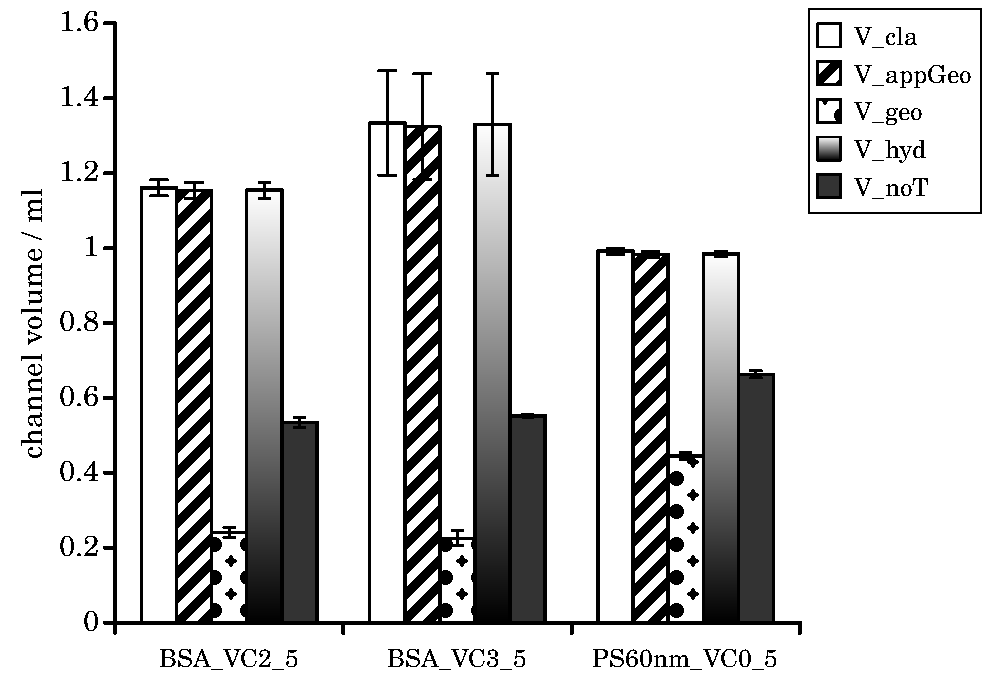
\includegraphics[width=\linewidth]{./images/data/eval_own_p12/ownData_V_p12.pdf}
      \subcaption{Calibration results for $V$}
    \end{subfigure}
  \end{center}
  \vspace*{-4ex}    
  \caption[Statistical results of $w$ and $V$ from all 5 calibration algorithms for assumed $\zP = \SI{12}{\percent}$]{
    Statistical results of $w$ and $V$ from all 5 calibration algorithms for assumed $\zP = \SI{12}{\percent}$
  }
 \label{fig:statCalibResP12}
\end{figure}
%%%%%%%%%%%%%%%%%%%%%%%%%%%%%%
%%% z% = 12
%%%%%%%%%%%%%%%%%%%%%%%%%%%%%
\begin{figure}[!hb]
  \begin{center}
    \begin{subfigure}{\subFigSize}
      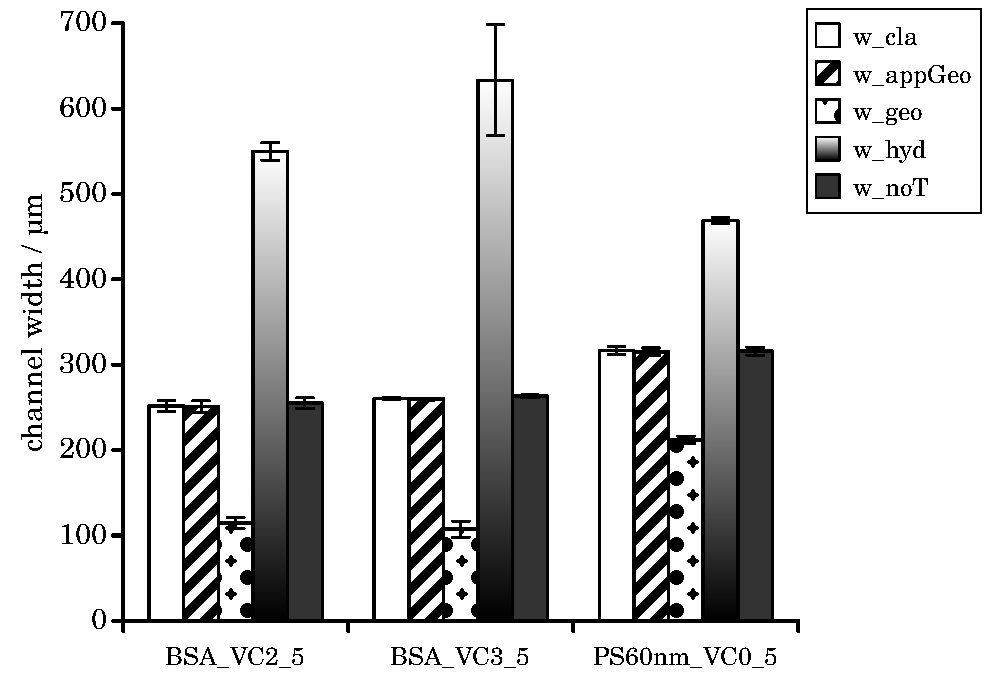
\includegraphics[width=\linewidth]{./images/data/eval_own_p12/ownData_w_p12.pdf}
      \subcaption{Calibration results for $w$}
      %      \label{subfig:calibRes_PS_VC0_5_w}
    \end{subfigure}
    \begin{subfigure}{\subFigSize}
      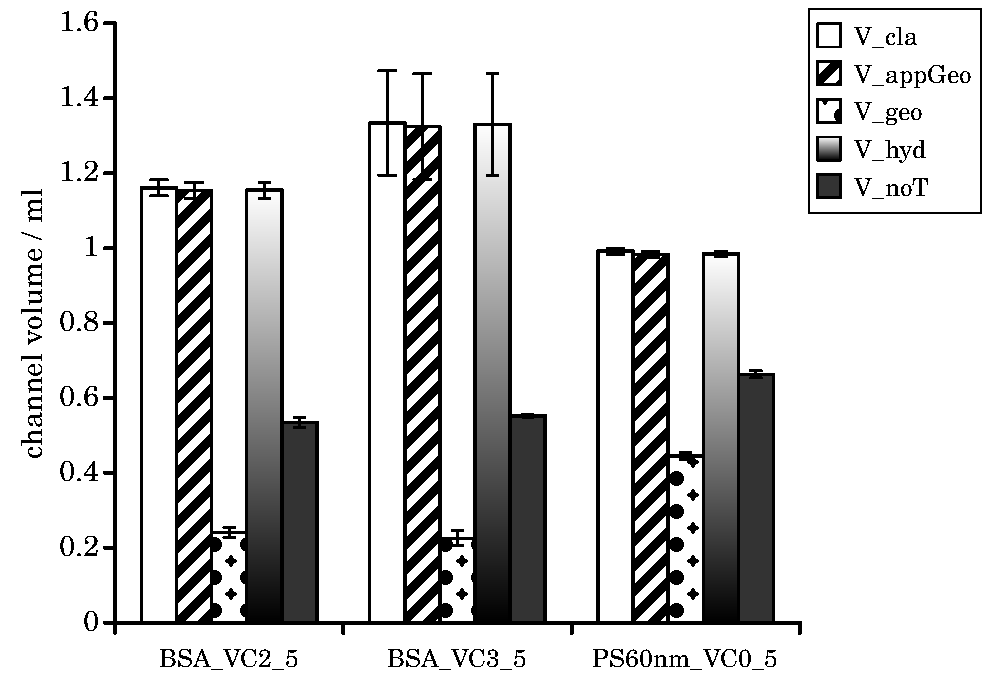
\includegraphics[width=\linewidth]{./images/data/eval_own_p12/ownData_V_p12.pdf}
      \subcaption{Calibration results for $V$}
    \end{subfigure}
  \end{center}
  \vspace*{-4ex}    
  \caption[Statistical results of $w$ and $V$ from all 5 calibration algorithms for assumed $\zP = \SI{16}{\percent}$]{
    Statistical results of $w$ and $V$ from all 5 calibration algorithms for assumed $\zP = \SI{16}{\percent}$
  }
\label{fig:statCalibResP16}
\end{figure}
%%%%%%%%%%%%%%%%%%%%%%%%%%%%%%%%%%%%%%%%%%%%%
%%% 
%%% Evaluated own results at z = 8 %
%%%
%%%%%%%%%%%%%%%%%%%%%%%%%%%%%%%%%%%%%%%%%%%%%
\section*{Single results of own calibration experiments with BSA and PS, 
  $\bm{\zP}$\thinspace=\thinspace8\thinspace\%}
\renewcommand{\subFigSize}{0.49\linewidth}
%\begin{landscape}
%\thispagestyle{empty}
%%%%%%%%%%%%%%%%%%%%%%%%%%%%%%
%%% BSA, Vc = 2.5 ml/min
%%%%%%%%%%%%%%%%%%%%%%%%%%%%%
%\begin{minipage}[t]{1.1\linewidth}
\begin{figure}[htp]
  \begin{center}
    \begin{subfigure}{\subFigSize}
      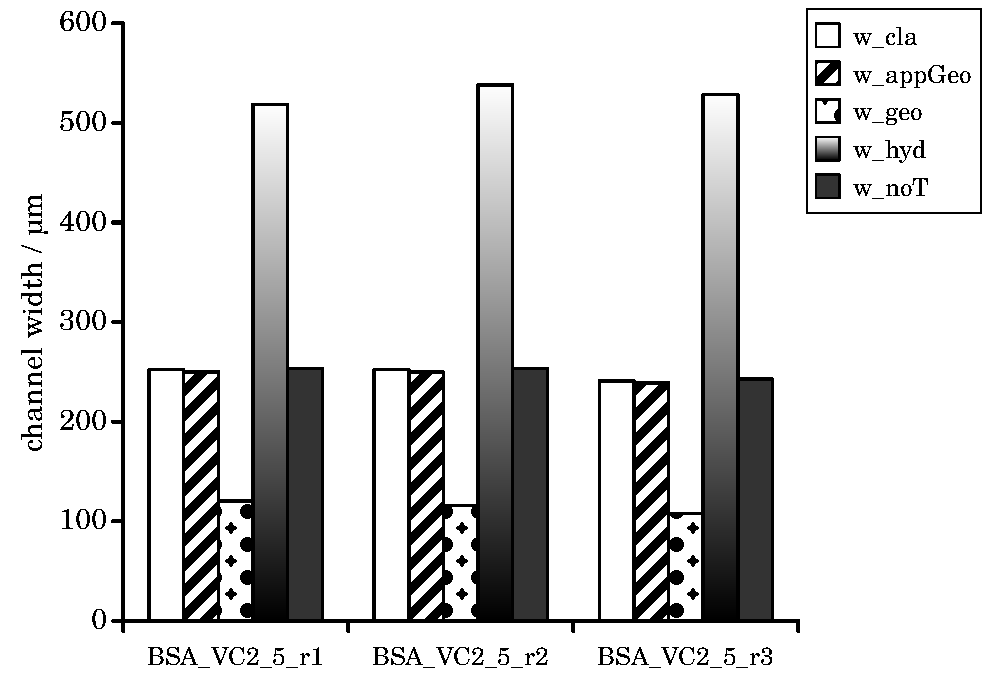
\includegraphics[width=\linewidth]{./images/data/eval_own_p8/calibW_BSA_VC_2_5_p8.pdf}
      \subcaption{Calibration results for $w$}
%      \label{subfig:calibRes_BSA_VC2_5_w}
    \end{subfigure}
    \begin{subfigure}{\subFigSize}
      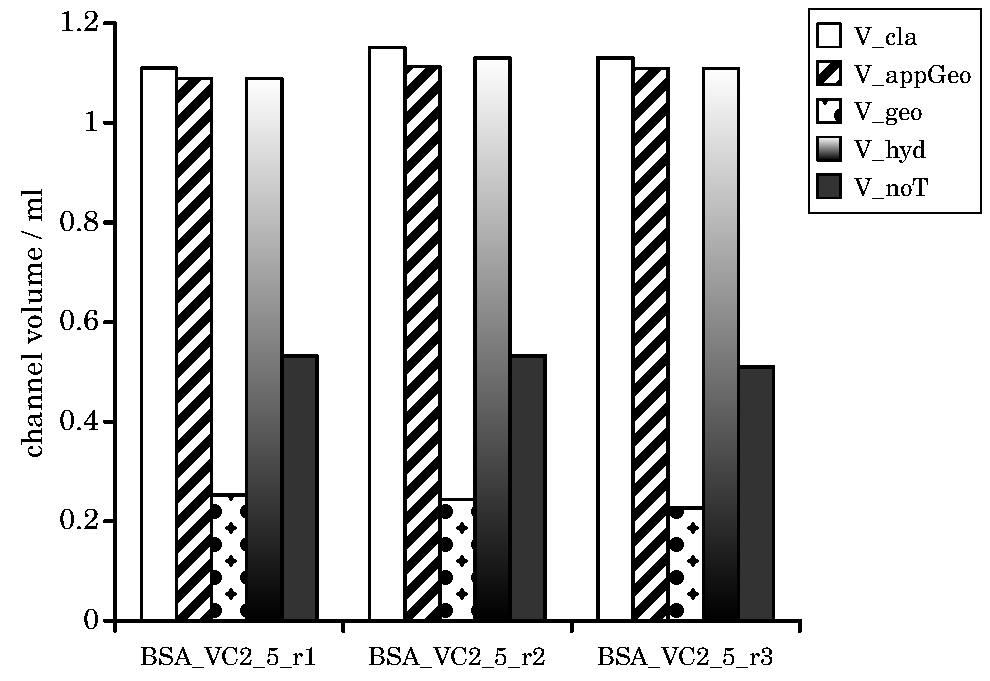
\includegraphics[width=\linewidth]{./images/data/eval_own_p8/calibV_BSA_VC_2_5_p8.pdf}
      \subcaption{Calibration results for $V$}
    \end{subfigure}
  \end{center}
  \vspace*{-4ex}    
  \caption[Results of $w$ and $V$ from all 5 calibration algorithms for BSA measurements at
  $\Vc = \SI{2.5}{\mlmin}$, $\zP = \SI{8}{\percent}$]{
    Results of $w$ and $V$ from all 5 calibration algorithms for BSA measurements at
    $\Vc = \SI{2.5}{\mlmin}$, $\zP = \SI{8}{\percent}$
  }
  \label{fig:calibRes_BSA_VC2_5}
\end{figure}  
%%%%%%%%%%%%%%%%%%%%%%%%%%%%%%
%%% BSA, Vc = 3.5 ml/min
%%%%%%%%%%%%%%%%%%%%%%%%%%%%%
\begin{figure}[htp]
  \begin{center}
    \begin{subfigure}{\subFigSize}
      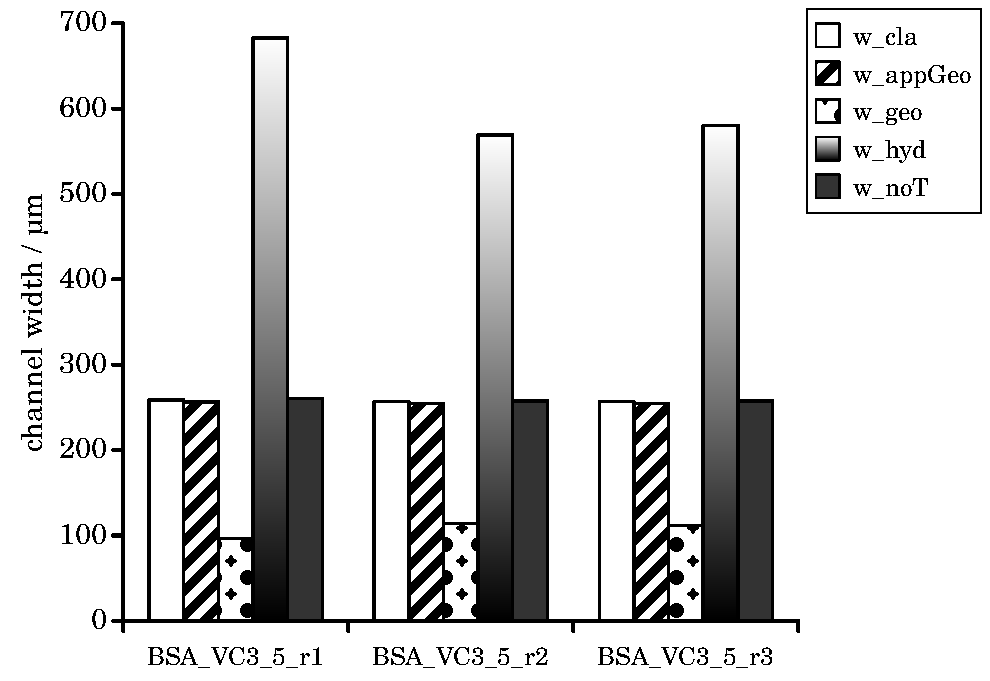
\includegraphics[width=\linewidth]{./images/data/eval_own_p8/calibW_BSA_VC_3_5_p8.pdf}
      \subcaption{Calibration results for $w$}
%      \label{subfig:calibRes_BSA_VC3_5_w}
    \end{subfigure}
    \begin{subfigure}{\subFigSize}
      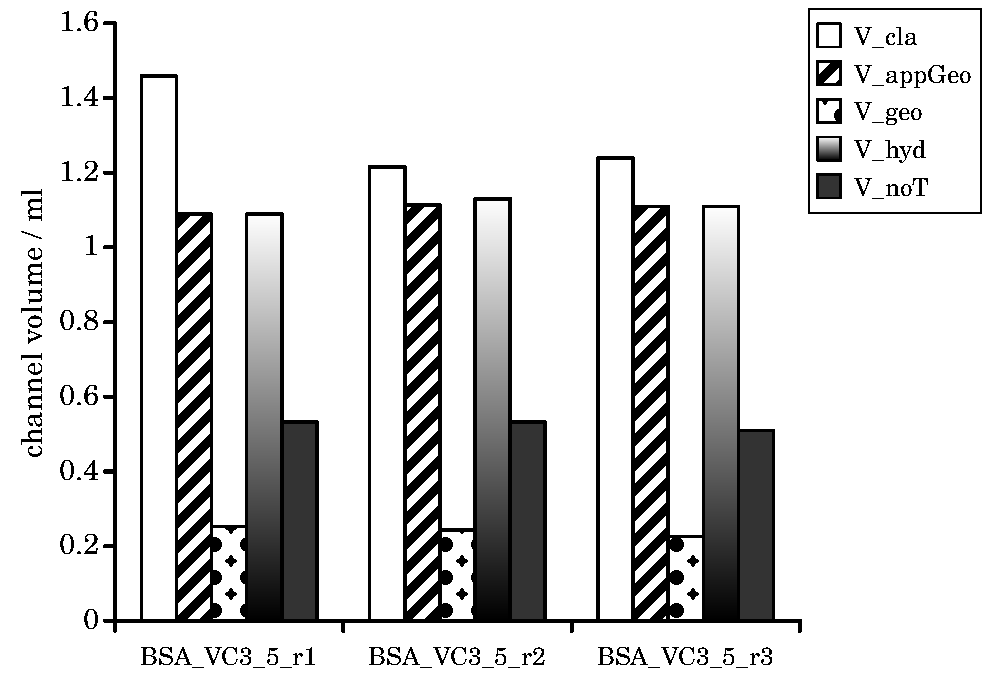
\includegraphics[width=\linewidth]{./images/data/eval_own_p8/calibV_BSA_VC_3_5_p8.pdf}
      \subcaption{Calibration results for $V$}
    \end{subfigure}
  \end{center}
  \vspace*{-4ex}    
  \caption[Results of $w$ and $V$ from all 5 calibration algorithms for BSA measurements at
  $\Vc = \SI{3.5}{\mlmin}$, $\zP = \SI{8}{\percent}$]{
    Results of $w$ and $V$ from all 5 calibration algorithms for BSA measurements at
    $\Vc = \SI{3.5}{\mlmin}$, $\zP = \SI{8}{\percent}$
  }
  \label{fig:calibRes_BSA_VC3_5}
\end{figure}
%%%%%%%%%%%%%%%%%%%%%%%%%%%%%%
%%% PS, Vc = 0.5 ml/min
%%%%%%%%%%%%%%%%%%%%%%%%%%%%%
\begin{figure}[!hb]
  \begin{center}
    \begin{subfigure}{\subFigSize}
      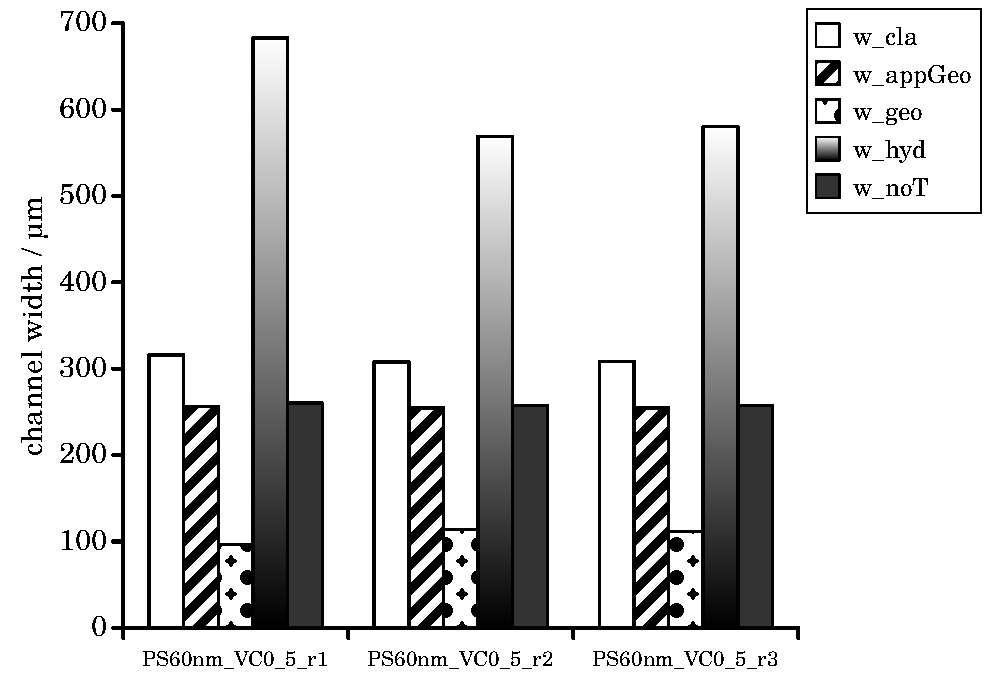
\includegraphics[width=\linewidth]{./images/data/eval_own_p8/calibW_PS_VC_0_5_p8.pdf}
      \subcaption{Calibration results for $w$}
      %      \label{subfig:calibRes_PS_VC0_5_w}
    \end{subfigure}
    \begin{subfigure}{\subFigSize}
      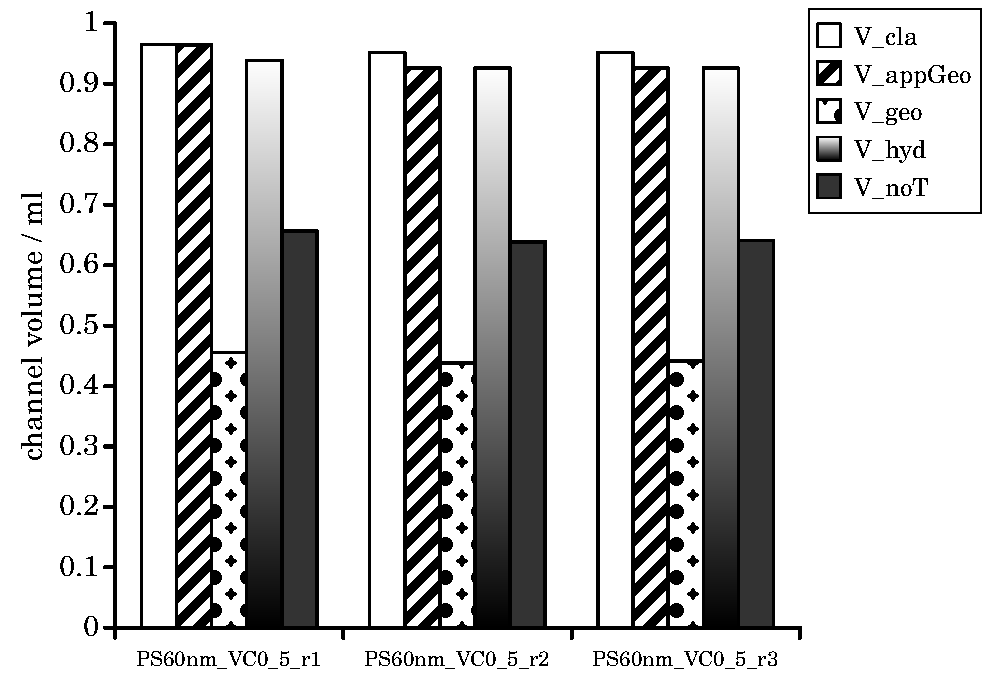
\includegraphics[width=\linewidth]{./images/data/eval_own_p8/calibV_PS_VC_0_5_p8.pdf}
      \subcaption{Calibration results for $V$}
    \end{subfigure}
  \end{center}
  \vspace*{-4ex}    
  \caption[Results of $w$ and $V$ from all 5 calibration algorithms for PS measurements at
  $\Vc = \SI{0.5}{\mlmin}$, $\zP = \SI{8}{\percent}$]{
    Results of $w$ and $V$ from all 5 calibration algorithms for PS measurements at
    $\Vc = \SI{0.5}{\mlmin}$, $\zP = \SI{8}{\percent}$
  }
  \label{fig:calibRes_PS_VC0_5_p8}
\end{figure}
%%%%%%%%%%%%%%%%%%%%%%%%%%%%%%%%%%%%%%%%%%%%%
%%% 
%%% Evaluated own results at z = 12 %
%%%
%%%%%%%%%%%%%%%%%%%%%%%%%%%%%%%%%%%%%%%%%%%%%
\section*{Single results of own calibration experiments with BSA and PS, 
$\bm{\zP}$\thinspace=\thinspace12\thinspace\%}
\renewcommand{\subFigSize}{0.49\linewidth}
%\begin{landscape}
%\thispagestyle{empty}
%%%%%%%%%%%%%%%%%%%%%%%%%%%%%%
%%% BSA, Vc = 2.5 ml/min
%%%%%%%%%%%%%%%%%%%%%%%%%%%%%
%\begin{minipage}[t]{1.1\linewidth}
\begin{figure}[htp]
  \begin{center}
    \begin{subfigure}{\subFigSize}
      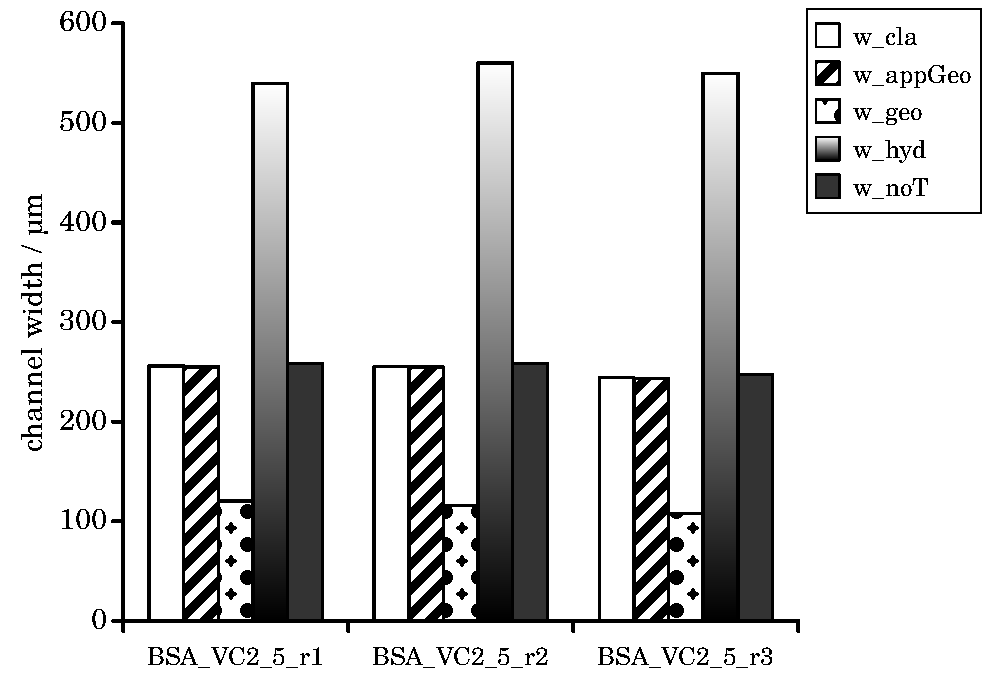
\includegraphics[width=\linewidth]{./images/data/eval_own_p12/calibW_BSA_VC_2_5_p12.pdf}
      \subcaption{Calibration results for $w$}
%      \label{subfig:calibRes_BSA_VC2_5_w}
    \end{subfigure}
    \begin{subfigure}{\subFigSize}
      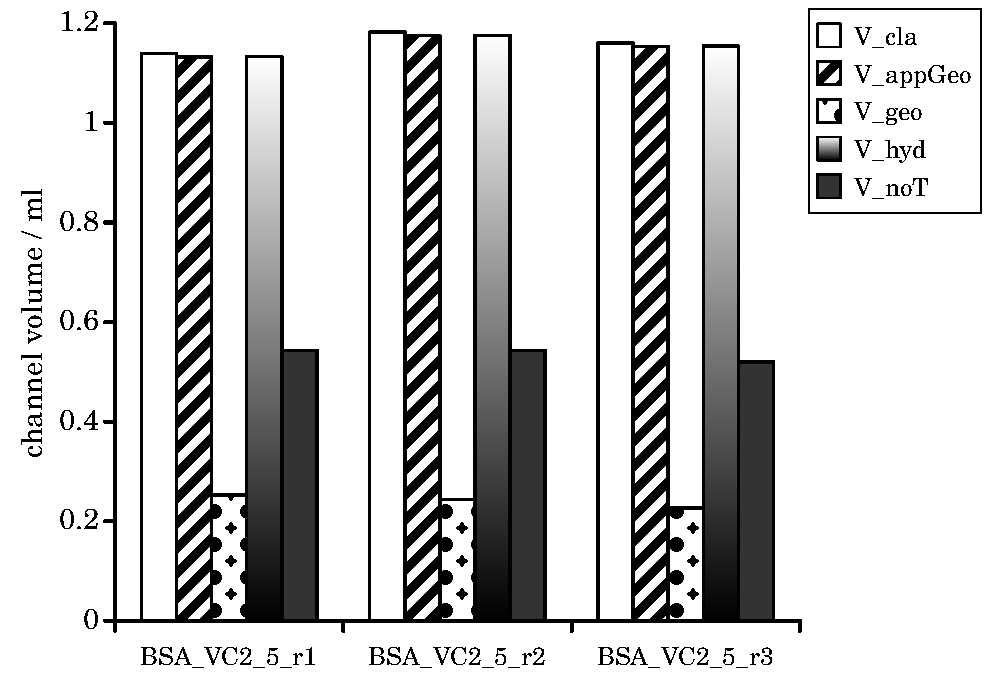
\includegraphics[width=\linewidth]{./images/data/eval_own_p12/calibV_BSA_VC_2_5_p12.pdf}
      \subcaption{Calibration results for $V$}
    \end{subfigure}
  \end{center}
  \vspace*{-4ex}    
  \caption[Results of $w$ and $V$ from all 5 calibration algorithms for BSA measurements at
   $\Vc = \SI{2.5}{\mlmin}$, $\zP = \SI{12}{\percent}$]{
     Results of $w$ and $V$ from all 5 calibration algorithms for BSA measurements at
     $\Vc = \SI{2.5}{\mlmin}$, $\zP = \SI{12}{\percent}$
}
\label{fig:calibRes_BSA_VC2_5}
\end{figure}  
%%%%%%%%%%%%%%%%%%%%%%%%%%%%%%
%%% BSA, Vc = 3.5 ml/min
%%%%%%%%%%%%%%%%%%%%%%%%%%%%%
\begin{figure}[htp]
  \begin{center}
    \begin{subfigure}{\subFigSize}
      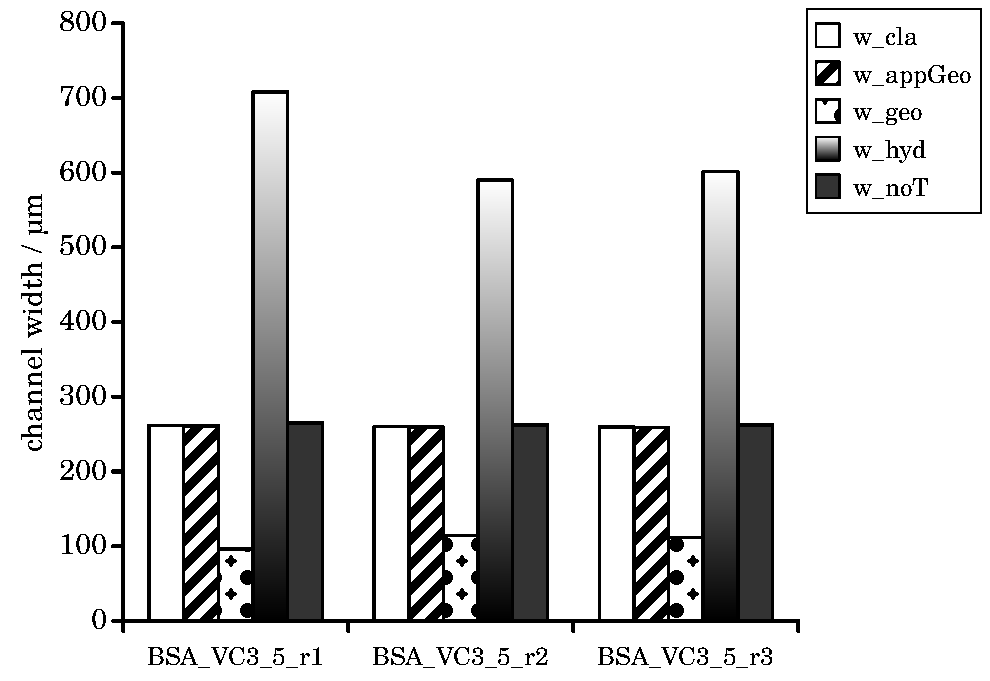
\includegraphics[width=\linewidth]{./images/data/eval_own_p12/calibW_BSA_VC_3_5_p12.pdf}
      \subcaption{Calibration results for $w$}
      \label{subfig:calibRes_BSA_VC3_5_w}
    \end{subfigure}
    \begin{subfigure}{\subFigSize}
      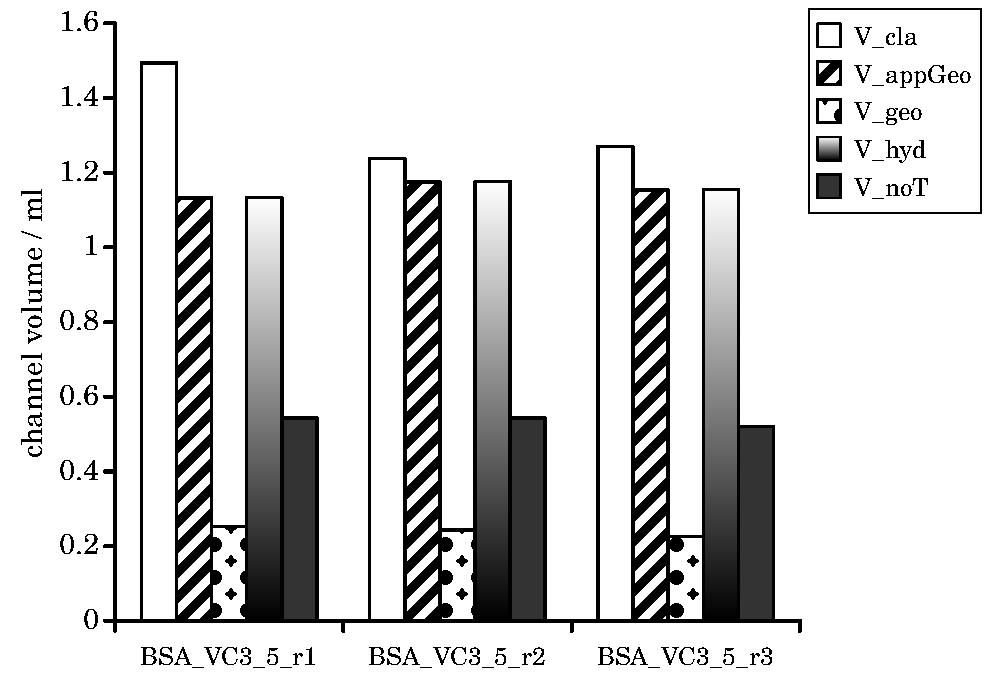
\includegraphics[width=\linewidth]{./images/data/eval_own_p12/calibV_BSA_VC_3_5_p12.pdf}
      \subcaption{Calibration results for $V$}
    \end{subfigure}
  \end{center}
  \vspace*{-4ex}    
  \caption[Results of $w$ and $V$ from all 5 calibration algorithms for BSA measurements at
  $\Vc = \SI{3.5}{\mlmin}$, $\zP = \SI{12}{\percent}$]{
    Results of $w$ and $V$ from all 5 calibration algorithms for BSA measurements at
    $\Vc = \SI{3.5}{\mlmin}$, $\zP = \SI{12}{\percent}$
  }
  \label{fig:calibRes_BSA_VC3_5}
\end{figure}
%%%%%%%%%%%%%%%%%%%%%%%%%%%%%%
%%% PS, Vc = 0.5 ml/min
%%%%%%%%%%%%%%%%%%%%%%%%%%%%%
\begin{figure}[!hb]
  \begin{center}
    \begin{subfigure}{\subFigSize}
      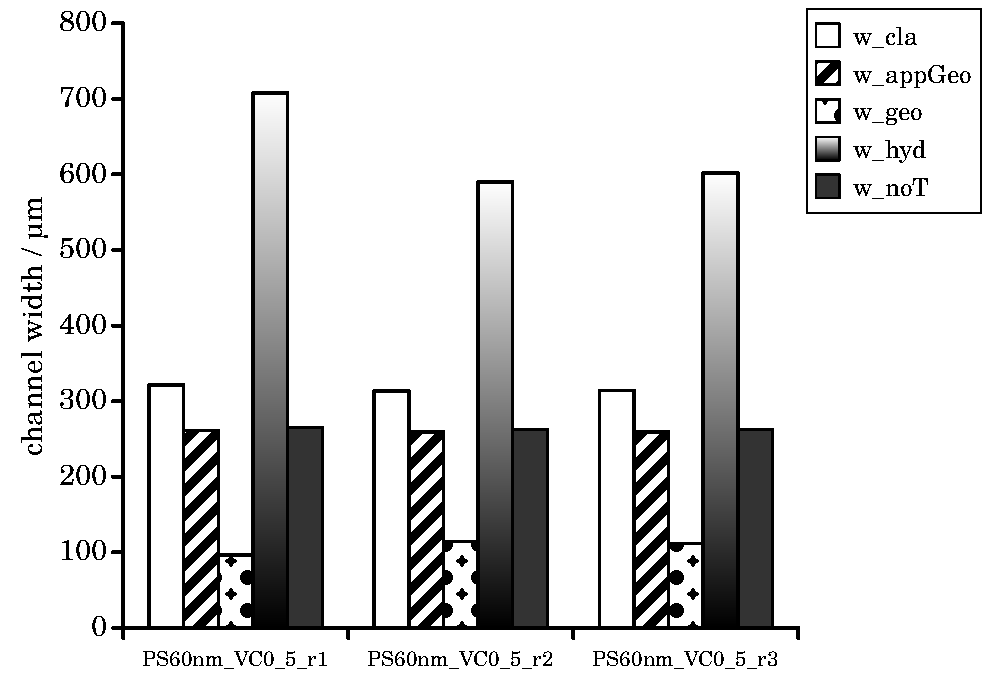
\includegraphics[width=\linewidth]{./images/data/eval_own_p12/calibW_PS_VC_0_5_p12.pdf}
      \subcaption{Calibration results for $w$}
%      \label{subfig:calibRes_PS_VC0_5_w}
    \end{subfigure}
    \begin{subfigure}{\subFigSize}
      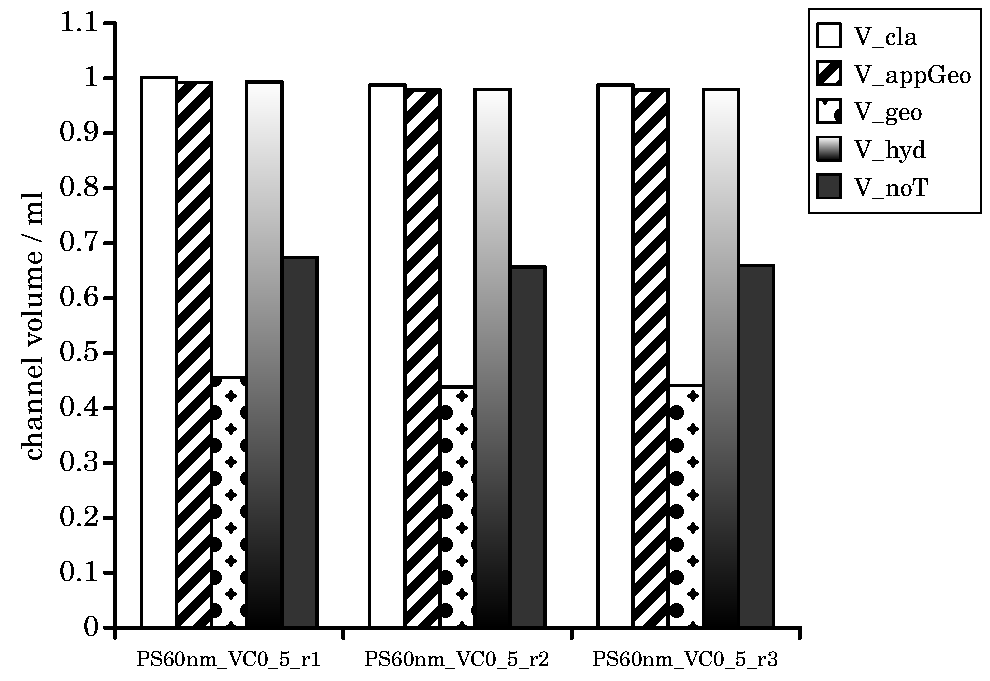
\includegraphics[width=\linewidth]{./images/data/eval_own_p12/calibV_PS_VC_0_5_p12.pdf}
      \subcaption{Calibration results for $V$}
    \end{subfigure}
 \end{center}
  \vspace*{-4ex}    
  \caption[Results of $w$ and $V$ from all 5 calibration algorithms for PS measurements at
  $\Vc = \SI{0.5}{\mlmin}$, $\zP = \SI{12}{\percent}$]{
    Results of $w$ and $V$ from all 5 calibration algorithms for PS measurements at
    $\Vc = \SI{0.5}{\mlmin}$, $\zP = \SI{12}{\percent}$
  }
  \label{fig:calibRes_PS_VC0_5}
\end{figure}
\FloatBarrier
%%%%%%%%%%%%%%%%%%%%%%%%%%%%%%%%%%%%%%%%%%%%%
%%% 
%%% Evaluated own results at z = 16 %
%%%
%%%%%%%%%%%%%%%%%%%%%%%%%%%%%%%%%%%%%%%%%%%%%
\section*{Single results of own calibration experiments with BSA and PS, 
  $\bm{\zP}$\thinspace=\thinspace16\thinspace\%}
\renewcommand{\subFigSize}{0.49\linewidth}
%\begin{landscape}
%\thispagestyle{empty}
%%%%%%%%%%%%%%%%%%%%%%%%%%%%%%
%%% BSA, Vc = 2.5 ml/min
%%%%%%%%%%%%%%%%%%%%%%%%%%%%%
%\begin{minipage}[t]{1.1\linewidth}
\begin{figure}[htp]
  \begin{center}
    \begin{subfigure}{\subFigSize}
      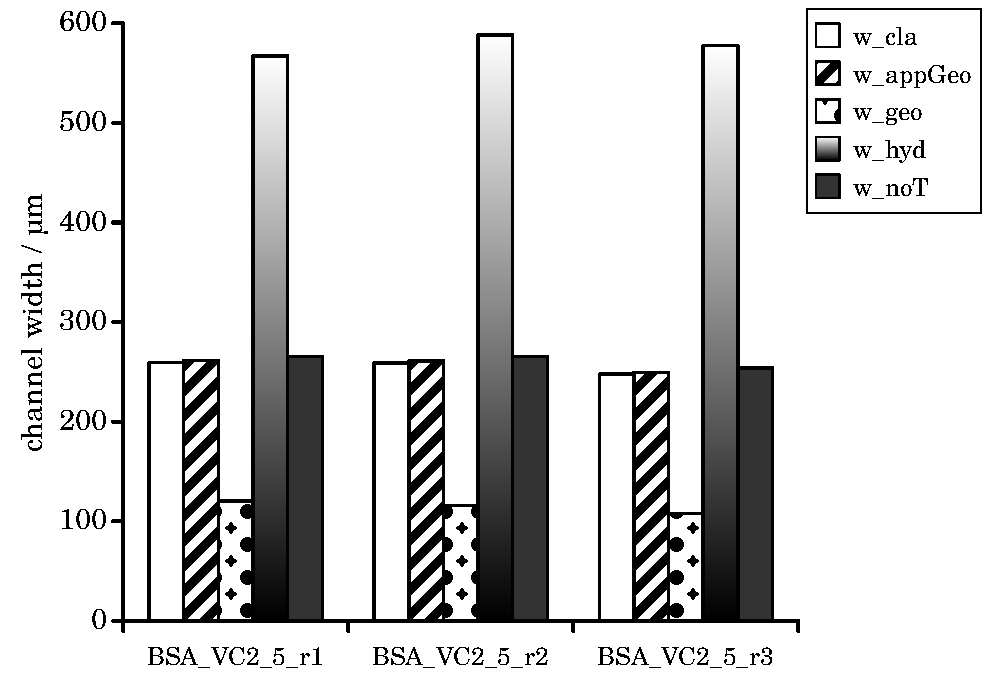
\includegraphics[width=\linewidth]{./images/data/eval_own_p16/calibW_BSA_VC_2_5_p16.pdf}
      \subcaption{Calibration results for $w$}
      %      \label{subfig:calibRes_BSA_VC2_5_w}
    \end{subfigure}
    \begin{subfigure}{\subFigSize}
      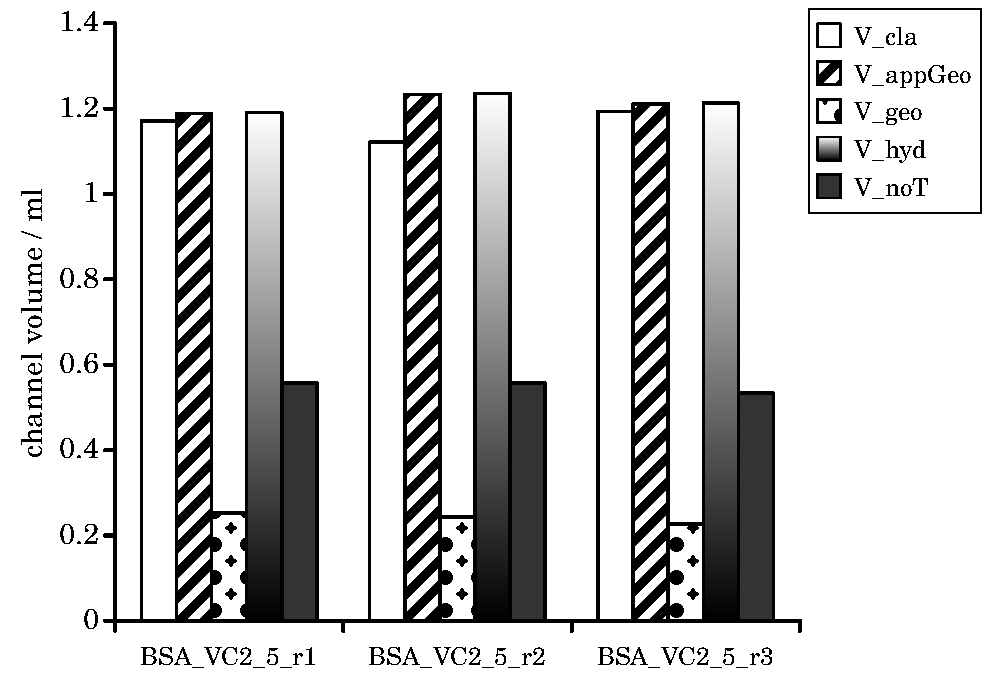
\includegraphics[width=\linewidth]{./images/data/eval_own_p16/calibV_BSA_VC_2_5_p16.pdf}
      \subcaption{Calibration results for $V$}
    \end{subfigure}
  \end{center}
  \vspace*{-4ex}    
  \caption[Results of $w$ and $V$ from all 5 calibration algorithms for BSA measurements at
  $\Vc = \SI{2.5}{\mlmin}$, $\zP = \SI{16}{\percent}$]{
    Results of $w$ and $V$ from all 5 calibration algorithms for BSA measurements at
    $\Vc = \SI{2.5}{\mlmin}$, $\zP = \SI{16}{\percent}$
  }
  \label{fig:calibRes_BSA_VC2_5_p16}
\end{figure}  
%%%%%%%%%%%%%%%%%%%%%%%%%%%%%%
%%% BSA, Vc = 3.5 ml/min
%%%%%%%%%%%%%%%%%%%%%%%%%%%%%
\begin{figure}[htp]
  \begin{center}
    \begin{subfigure}{\subFigSize}
      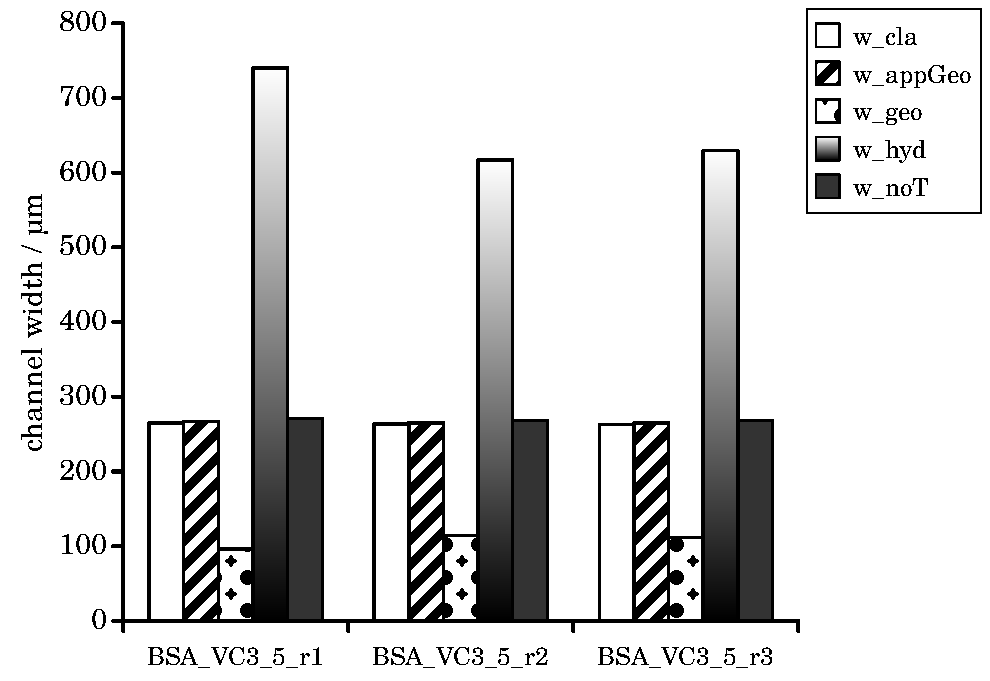
\includegraphics[width=\linewidth]{./images/data/eval_own_p16/calibW_BSA_VC_3_5_p16.pdf}
      \subcaption{Calibration results for $w$}
      \label{subfig:calibRes_BSA_VC3_5_w}
    \end{subfigure}
    \begin{subfigure}{\subFigSize}
      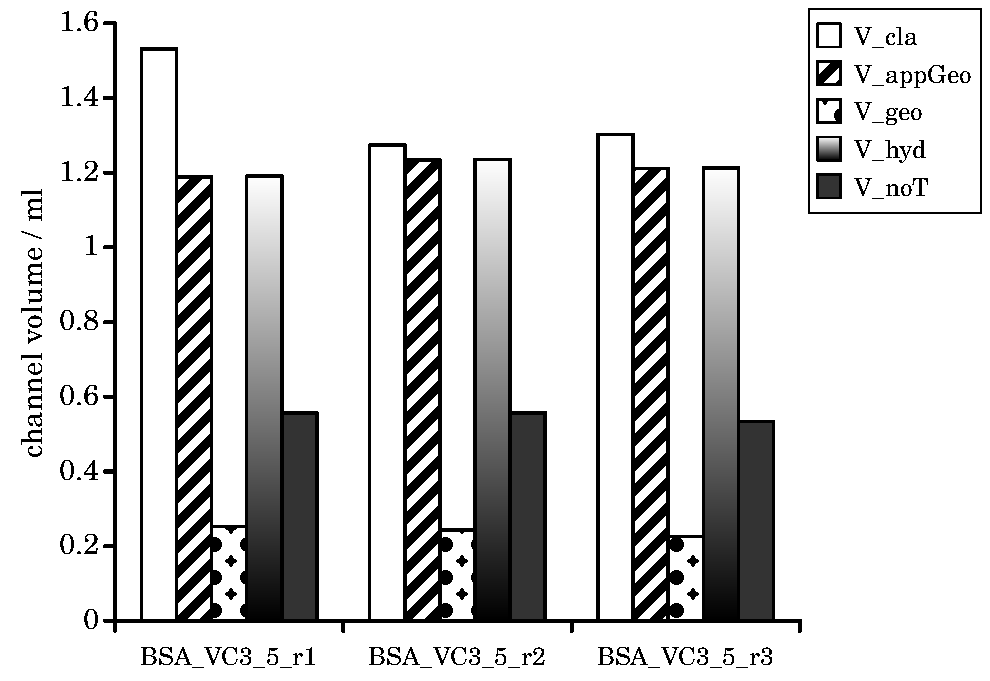
\includegraphics[width=\linewidth]{./images/data/eval_own_p16/calibV_BSA_VC_3_5_p16.pdf}
      \subcaption{Calibration results for $V$}
    \end{subfigure}
  \end{center}
  \vspace*{-4ex}    
  \caption[Results of $w$ and $V$ from all 5 calibration algorithms for BSA measurements at
  $\Vc = \SI{3.5}{\mlmin}$, $\zP = \SI{16}{\percent}$]{
    Results of $w$ and $V$ from all 5 calibration algorithms for BSA measurements at
    $\Vc = \SI{3.5}{\mlmin}$, $\zP = \SI{16}{\percent}$
  }
  \label{fig:calibRes_BSA_VC3_5_p16}
\end{figure}
%%%%%%%%%%%%%%%%%%%%%%%%%%%%%%
%%% PS, Vc = 0.5 ml/min
%%%%%%%%%%%%%%%%%%%%%%%%%%%%%
\begin{figure}[!hb]
  \begin{center}
    \begin{subfigure}{\subFigSize}
      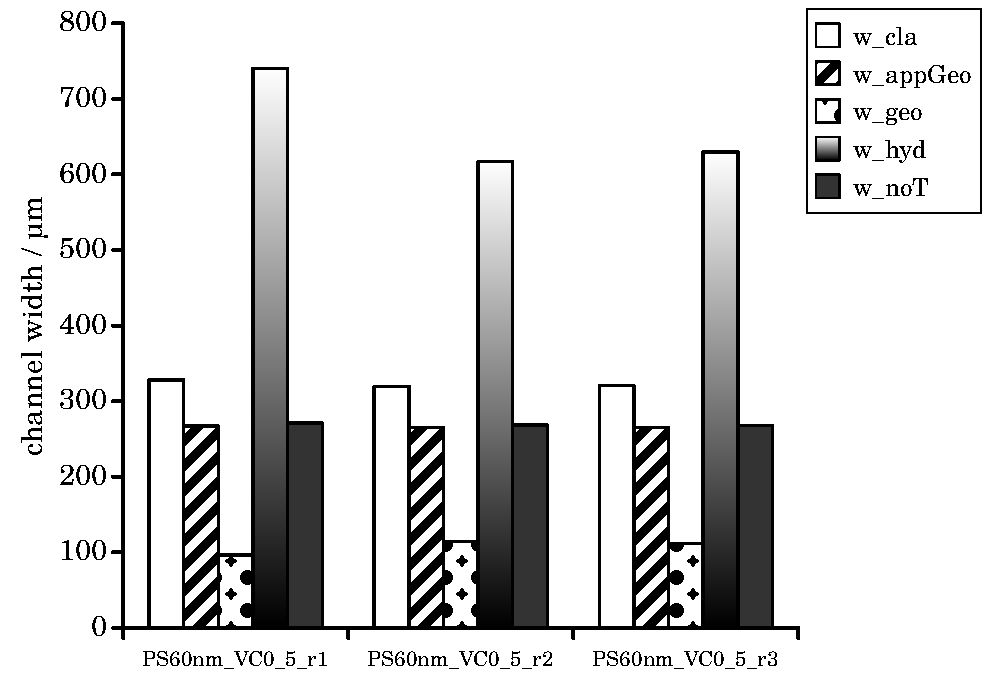
\includegraphics[width=\linewidth]{./images/data/eval_own_p16/calibW_PS_VC_0_5_p16.pdf}
      \subcaption{Calibration results for $w$}
      %      \label{subfig:calibRes_PS_VC0_5_w}
    \end{subfigure}
    \begin{subfigure}{\subFigSize}
      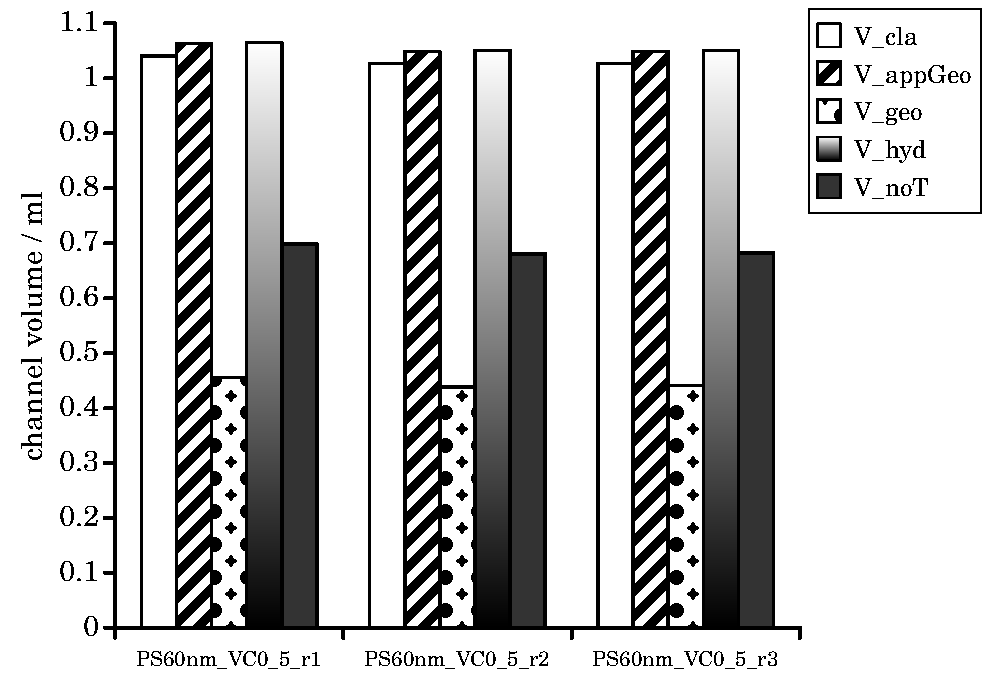
\includegraphics[width=\linewidth]{./images/data/eval_own_p16/calibV_PS_VC_0_5_p16.pdf}
      \subcaption{Calibration results for $V$}
    \end{subfigure}
  \end{center}
  \vspace*{-4ex}    
  \caption[Results of $w$ and $V$ from all 5 calibration algorithms for PS measurements at
  $\Vc = \SI{0.5}{\mlmin}$, $\zP = \SI{16}{\percent}$]{
    Results of $w$ and $V$ from all 5 calibration algorithms for PS measurements at
    $\Vc = \SI{0.5}{\mlmin}$, $\zP = \SI{16}{\percent}$
  }
  \label{fig:calibRes_PS_VC0_5_16}
\end{figure}
\FloatBarrier
%%%%%%%%%%%%%%%%%%%%%%%%%%%%%%%%%%%%%%%%%%%%%
%%% 
%%% Evaluated own results at z = 8 %
%%%
%%%%%%%%%%%%%%%%%%%%%%%%%%%%%%%%%%%%%%%%%%%%%
\section*{Single results of calibration experiments with literature data, 
  $\bm{\zP}$\thinspace=\thinspace8\thinspace\%}
\begin{figure}[H]
  \begin{center}
    \begin{subfigure}{.75\linewidth}
%      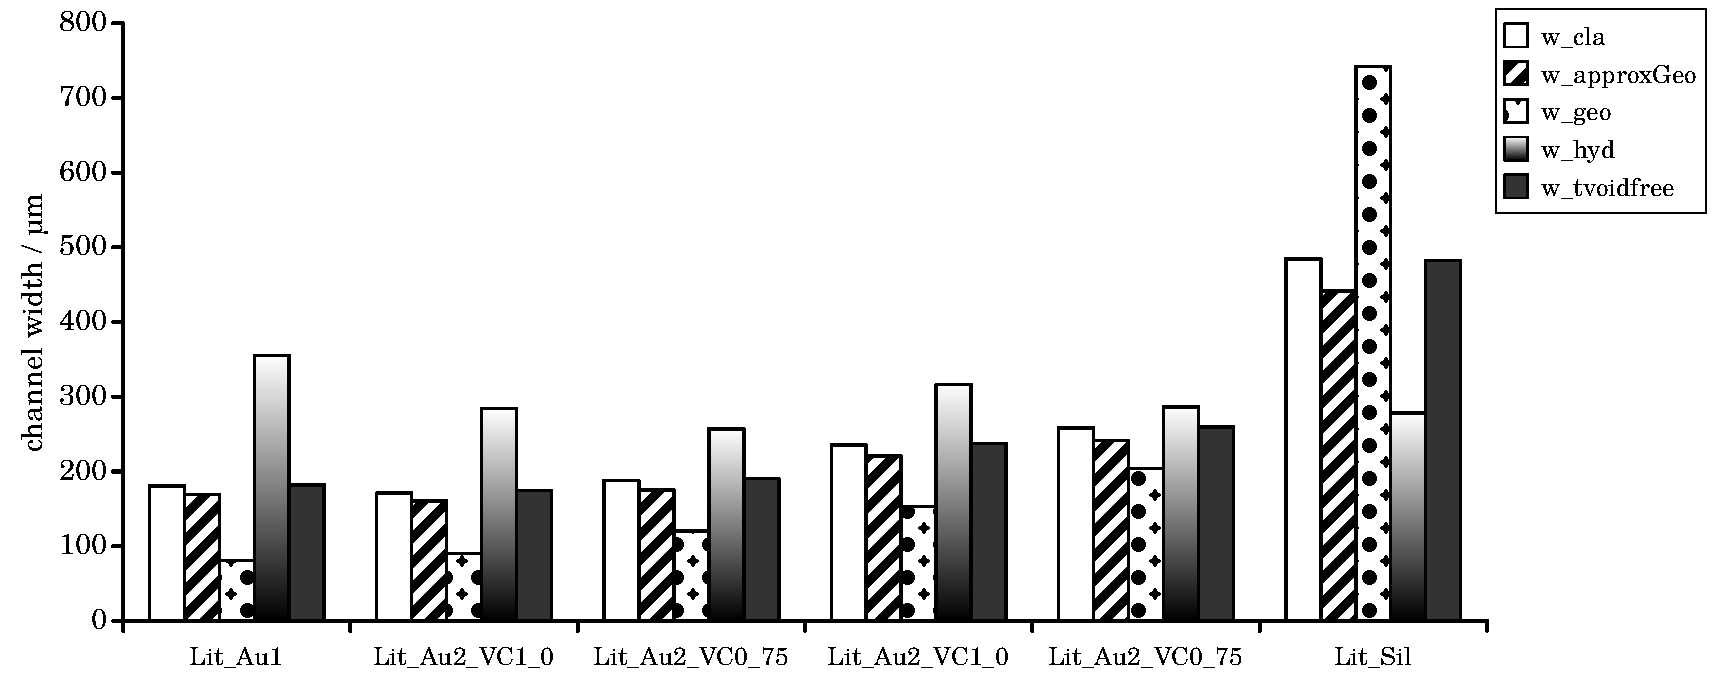
\includegraphics[width=\linewidth]{\imgpath/Fig7/img_calibW_LitData1.pdf} 
      \subcaption{$w$ for data from Table 3}
    \end{subfigure}\\
    \begin{subfigure}{.75\linewidth}
 %     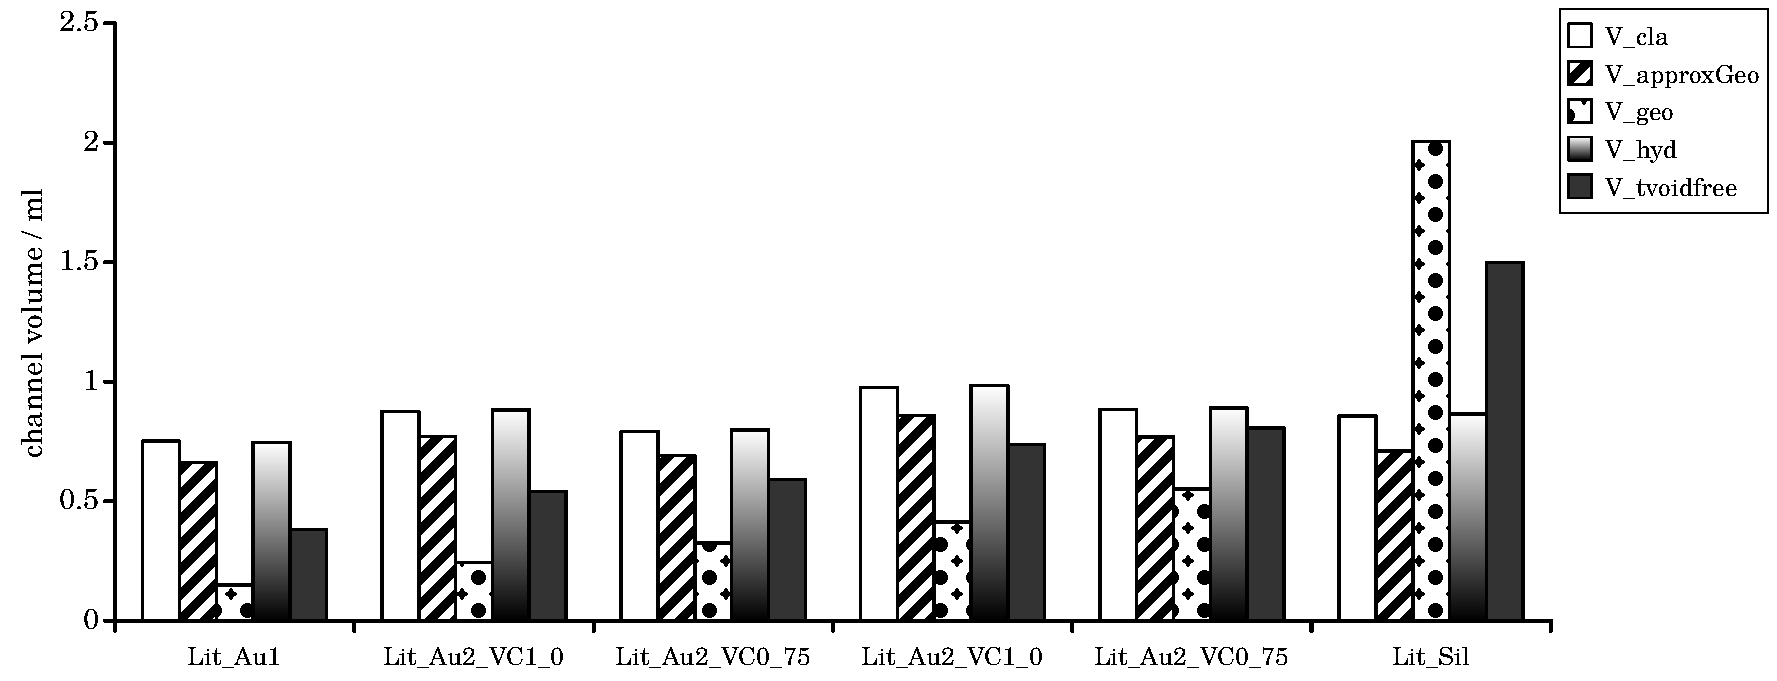
\includegraphics[width=\linewidth]{\imgpath/Fig7/img_calibV_LitData1.pdf} 
      \subcaption{$V$ for data from Table 3}
    \end{subfigure}\\
    \begin{subfigure}{.75\linewidth}
  %    \includegraphics[width=\linewidth]{\imgpath/Fig7/img_calibW_LitData2.pdf} 
      \subcaption{$w$ for data from Table 4}
    \end{subfigure}\\
    \begin{subfigure}{.75\linewidth}
   %   \includegraphics[width=\linewidth]{\imgpath/Fig7/img_calibV_LitData2.pdf} 
      \subcaption{$V$ for data from Table 4}
    \end{subfigure}
  \end{center}
  \caption[Results of calibration algorithms with literature data
  ]{Results of calibration algorithms with literature data}
  \label{fig:LitDataResults_p8}
\end{figure}
\clearpage

%%%%%%%%%%%%%%%%%%%%%%%%%%%%%%%%%%%%%%%%%%%%%
%%% 
%%% Evaluated own results at z = 16 %
%%%
%%%%%%%%%%%%%%%%%%%%%%%%%%%%%%%%%%%%%%%%%%%%%
\section*{Single results of calibration experiments with literature data, 
  $\bm{\zP}$\thinspace=\thinspace16\thinspace\%}

\begin{figure}[H]
  \begin{center}
    \begin{subfigure}{.75\linewidth}
      %      \includegraphics[width=\linewidth]{\imgpath/Fig7/img_calibW_LitData1.pdf} 
      \subcaption{$w$ for data from Table 3}
    \end{subfigure}\\
    \begin{subfigure}{.75\linewidth}
      %     \includegraphics[width=\linewidth]{\imgpath/Fig7/img_calibV_LitData1.pdf} 
      \subcaption{$V$ for data from Table 3}
    \end{subfigure}\\
    \begin{subfigure}{.75\linewidth}
      %    \includegraphics[width=\linewidth]{\imgpath/Fig7/img_calibW_LitData2.pdf} 
      \subcaption{$w$ for data from Table 4}
    \end{subfigure}\\
    \begin{subfigure}{.75\linewidth}
      %   \includegraphics[width=\linewidth]{\imgpath/Fig7/img_calibV_LitData2.pdf} 
      \subcaption{$V$ for data from Table 4}
    \end{subfigure}
  \end{center}
  \caption[Results of calibration algorithms with literature data
  ]{Results of calibration algorithms with literature data}
  \label{fig:LitDataResults_p16}
\end{figure}

\FloatBarrier
%\clearpage
\newgeometry{margin=1.3cm}
%\needspace{20em}
\section*{Deviation influences}
%\lipsum
\begin{figure}[H]
  \begin{center}
    \includegraphics[width=.925\linewidth]{./images/deltaAnalysis.pdf}
  \end{center}
  \vspace*{-3ex}
  \caption[Parameter deviation analysis, example for sample BSA\_VC2\_5\_r1]{Parameter deviation analysis, example for sample 
  BSA\_VC2\_5\_r1}
  \label{fig:DeviationAnalysis}
\end{figure}
\FloatBarrier
\restoregeometry
%%%%%%%%%%%%%%%%%%%%%%%%%%%%%%%%%%%%%%%%%%%%%%%%%%%%%%%
%%% 
%%% Evaluated own results for assumed correct tvoid
%%%
%%%%%%%%%%%%%%%%%%%%%%%%%%%%%%%%%%%%%%%%%%%%%%%%%%%%%%%%
\section*{Single results of own calibration experiments with calculated $\tvoid$, 
  $\bm{\zP}$\thinspace=\thinspace12\thinspace\%}
\renewcommand{\subFigSize}{0.49\linewidth}
%\begin{landscape}
%\thispagestyle{empty}
%%%%%%%%%%%%%%%%%%%%%%%%%%%%%%
%%% BSA, Vc = 2.5 ml/min
%%%%%%%%%%%%%%%%%%%%%%%%%%%%%
%\begin{minipage}[t]{1.1\linewidth}
\begin{figure}[htp]
  \begin{center}
    \begin{subfigure}{\subFigSize}
%      \includegraphics[width=\linewidth]{./images/data/eval_own_p16/calibW_BSA_VC_2_5_p16.pdf}
      \subcaption{Calibration results for $w$}
      %      \label{subfig:calibRes_BSA_VC2_5_w}
    \end{subfigure}
    \begin{subfigure}{\subFigSize}
%      \includegraphics[width=\linewidth]{./images/data/eval_own_p16/calibV_BSA_VC_2_5_p16.pdf}
      \subcaption{Calibration results for $V$}
    \end{subfigure}
  \end{center}
  \vspace*{-4ex}    
  \caption[Results of $w$ and $V$ from all 5 calibration algorithms for BSA measurements at
  $\Vc = \SI{2.5}{\mlmin}$, $\zP = \SI{16}{\percent}$]{
    Results of $w$ and $V$ from all 5 calibration algorithms for BSA measurements at
    $\Vc = \SI{2.5}{\mlmin}$, $\zP = \SI{16}{\percent}$
  }
  \label{fig:calibRes_BSA_VC2_5_tvoidCorr}
\end{figure}  
%%%%%%%%%%%%%%%%%%%%%%%%%%%%%%
%%% BSA, Vc = 3.5 ml/min
%%%%%%%%%%%%%%%%%%%%%%%%%%%%%
\begin{figure}[htp]
  \begin{center}
    \begin{subfigure}{\subFigSize}
%      \includegraphics[width=\linewidth]{./images/data/eval_own_p16/calibW_BSA_VC_3_5_p16.pdf}
      \subcaption{Calibration results for $w$}
%      \label{subfig:calibRes_BSA_VC3_5_w}
    \end{subfigure}
    \begin{subfigure}{\subFigSize}
%      \includegraphics[width=\linewidth]{./images/data/eval_own_p16/calibV_BSA_VC_3_5_p16.pdf}
      \subcaption{Calibration results for $V$}
    \end{subfigure}
  \end{center}
  \vspace*{-4ex}    
  \caption[Results of $w$ and $V$ from all 5 calibration algorithms for BSA measurements at
  $\Vc = \SI{3.5}{\mlmin}$, $\zP = \SI{16}{\percent}$]{
    Results of $w$ and $V$ from all 5 calibration algorithms for BSA measurements at
    $\Vc = \SI{3.5}{\mlmin}$, $\zP = \SI{16}{\percent}$
  }
  \label{fig:calibRes_BSA_VC3_5_tvoidCorr}
\end{figure}
%%%%%%%%%%%%%%%%%%%%%%%%%%%%%%
%%% PS, Vc = 0.5 ml/min
%%%%%%%%%%%%%%%%%%%%%%%%%%%%%
\begin{figure}[!hb]
  \begin{center}
    \begin{subfigure}{\subFigSize}
%      \includegraphics[width=\linewidth]{./images/data/eval_own_p16/calibW_PS_VC_0_5_p16.pdf}
      \subcaption{Calibration results for $w$}
      %      \label{subfig:calibRes_PS_VC0_5_w}
    \end{subfigure}
    \begin{subfigure}{\subFigSize}
%      \includegraphics[width=\linewidth]{./images/data/eval_own_p16/calibV_PS_VC_0_5_p16.pdf}
      \subcaption{Calibration results for $V$}
    \end{subfigure}
  \end{center}
  \vspace*{-4ex}    
  \caption[Results of $w$ and $V$ from all 5 calibration algorithms for PS measurements at
  $\Vc = \SI{0.5}{\mlmin}$, $\zP = \SI{16}{\percent}$]{
    Results of $w$ and $V$ from all 5 calibration algorithms for PS measurements at
    $\Vc = \SI{0.5}{\mlmin}$, $\zP = \SI{16}{\percent}$
  }
  \label{fig:calibRes_PS_VC0_5_tvoidCorr}
\end{figure}
%\KOMAoptions{paper=a4}
%\recalctypearea
%\clearpage
%\lipsum